\pdfoutput=1
\documentclass[11pt]{amsart}
\usepackage{amsmath,amssymb,amsthm,booktabs}
\usepackage{tikz}
\usepackage[margin=1.2in]{geometry}
\usepackage[colorlinks=true,linkcolor=blue,citecolor=blue,urlcolor=blue]{hyperref}
\hypersetup{pdfauthor={Bernd Johannes Wuebben},pdftitle={Fan symmetries and exceptional collections on toric Fano varieties}}
\setlength{\emergencystretch}{2em}
\newtheorem{theorem}{Theorem}[section]
\newtheorem{proposition}[theorem]{Proposition}
\newtheorem{lemma}[theorem]{Lemma}
\newtheorem{corollary}[theorem]{Corollary}
\theoremstyle{definition}
\newtheorem{question}[theorem]{Question}
\newcommand{\C}{\mathbb C}
\newcommand{\Z}{\mathbb Z}
\DeclareMathOperator{\Jac}{Jac}
\DeclareMathOperator{\Spec}{Spec}
\title[Fan symmetries and exceptional collections]{Fan symmetries and exceptional collections \\on toric Fano varieties}
\author{Bernd Johannes Wuebben}
\date{November 17, 2026\\This version: November 18, 2026}
\subjclass[2020]{14M25, 14F08, 53D45, 19E08}
\keywords{Toric Fano variety, quantum cohomology, Gamma class, exceptional collection, permutation lattice}
\begin{document}
\begin{abstract}
Every smooth projective complex toric Fano variety has a full exceptional collection permuted by the automorphism group of its fan. We construct a semisimple point of big quantum cohomology fixed by this group. At each admissible lifted phase the objects can be chosen so that their individual classes give the integral Gamma asymptotic basis indexed by the primitive idempotents at that point. Distinct objects with the same Euler eigenvalue are orthogonal in every degree. One mirror equivalence identifies the fan action on Lefschetz thimbles with toric pullback on perfect complexes. Testing a second equivalence on mirror disks associated with ample polytopes determines the integral classes of its thimble images. Comparing the equivalences recovers the fan action on these images. The objects have rational models on the split variety, and their Galois orbits give division-algebra components on every form in characteristic zero. Over the locus in the nonarchimedean fixed quantum base where the number of distinct Euler eigenvalues is maximal, the reduced Euler cover is the quotient of the primitive-idempotent cover by the fan group. Its connected components give the local equivariant Hodge atoms.
\end{abstract}
\maketitle
\enlargethispage{2pt}
\begin{center}\small Equivariant Quantum Geometry, Paper 01\end{center}

\section{Introduction}
Consider inversion on the dense torus of $\mathbb P^1$. It exchanges the two torus-fixed points of the compactification. Yet it fixes both generators $[\mathcal O]$ and $[\mathcal O(1)]$ of $K_0(\mathbb P^1)$. The two critical points of the mirror function $x+x^{-1}$ give the correct action: both $1$ and $-1$ are fixed. This example suggests looking for an integral basis indexed by critical points of a mirror which retains the symmetry of the original variety.

Let $\Sigma$ be a complete smooth fan in a lattice $N$, let $X=X_\Sigma$ be projective and Fano, and let $G$ be a finite group preserving the fan. We use inverse pullback for the left action on cohomology, bundles and complexes. Write $H=H^{\mathrm{even}}(X;\C)$ and $\mu=\dim H$. A semisimple quantum product on $H$ exhibits it as a product of $\mu$ copies of $\C$. The units in the individual factors are its primitive idempotents. At a parameter fixed by $G$ these form a finite $G$-set.

The question of Merkurjev and Panin asks whether the geometric $K$-group of an arithmetic toric variety is a permutation Galois lattice. Castravet and Tevelev asked for a categorical realization by exceptional objects. A full exceptional collection is an ordered sequence generating $D^b\mathrm{Coh}(X)$, with $\mathrm{RHom}(E_j,E_i)=0$ for $j>i$ and $\mathrm{RHom}(E_i,E_i)=\C$ in degree zero. To recover a permutation on the integral group, it suffices that automorphisms permute its members up to isomorphism. Erman, Hanlon, Liu and Zheng constructed such a collection of line bundles in the Cox category of a projective toric variety \cite{EHLZ}. We work in the ordinary derived category of the Fano variety itself.

\begin{theorem}\label{thm:maincombined}
There is a $G$-fixed semisimple parameter $\tau$ in convergent big quantum cohomology on the large-radius branch of $X$. Write $S$ for its primitive idempotents and $u_s$ for the eigenvalue of quantum multiplication by the Euler field on the factor $s$. At each admissible lifted phase $\varphi$ there is a full exceptional collection $(E_s)_{s\in S}$ in $D^b\mathrm{Coh}(X)$ such that
\[
      (f_{g^{-1}})^*E_s\simeq E_{gs},\qquad
      \mathrm{RHom}(E_s,E_{s'})=0\quad(s\ne s',\ u_s=u_{s'}).
\]
Its order is that of decreasing $\operatorname{Im}(e^{-i\varphi}u_s)$, with arbitrary order among tied values. With compatible signs of the normalized idempotents, the Gamma-framed sections of the $[E_s]$ are the individual normalized asymptotic columns. In particular $s\mapsto[E_s]$ induces an isomorphism $\Z[S]\simeq K_0(X)$ of integral $G$-modules.
\end{theorem}

Here $f_g$ denotes the toric automorphism of $X$. A phase is admissible if distinct Euler values have distinct projected imaginary parts; lifting the angle specifies the branch for the asymptotic solutions. Equal Euler values occur naturally: all primitive factors in one $G$-orbit have the same eigenvalue. Distinguishing their objects is part of the assertion. The basis assertion alone holds at every fixed semisimple point on this branch at which the descendant framing is defined compatibly with $G$ (Section~\ref{sec:lattice}). The categorical construction selects a particular fixed point.

The proof has three parts. First we construct an invariant Morse deformation of the toric Laurent polynomial and identify its persistent critical scheme with the analytic big quantum algebra. The point must lie on the fixed locus; semisimplicity elsewhere would allow all symmetries to be broken. Gui, Qin, Shen and Xiong proved a permutation theorem for ungraded rational cohomology of all smooth projective toric varieties \cite[Theorem~1.2]{GQSX}. Their invariant Morse argument motivates the local construction here. The analytic identification uses the mirror theorem of Coates, Corti, Iritani and Tseng \cite{CCIT}. Once the fixed point has been found, the integral structure of Galkin and Iritani gives the asymptotic lattice \cite{GI}.

Fang and Zhou construct a full exceptional collection from thimbles of a small toric mirror with distinct critical values \cite[Proposition~5.4]{FZ}. At a parameter fixed by a group acting trivially on the value plane, distinct critical values force every critical point to be fixed. To realize a nontrivial permutation we must allow several Morse points over one value. A large Laurent perturbation at infinity can change the reference fibre even on $\mathbb P^1$. Section~\ref{sec:compactmirror} keeps that fibre fixed and separates coincident critical values while retaining the same geometric thimbles. Ordering two tied disks either way proves both morphism vanishings. A Weinstein handle presentation identifies these disks as generators. For the passage to a cotangent bundle we use the geometric comparison of Fang, Hu, Sun and Zhou \cite{FHSZ}, building on the hypersurface skeleta of Gammage--Shende and Zhou \cite{GS,Zhou}. We choose an invariant convex potential and follow the entire marked fibre in that comparison. This identifies its core with the fan conic link while transporting the group action and the gradings of the individual disks. At this endpoint a fan symmetry acts by a diffeomorphism of the angle torus; the coherent--constructible correspondence identifies this action with toric pullback (Section~\ref{sec:coherenttransport}).

Finally, the integral comparison must associate each asymptotic column with the class of an individual object. We use a second equivalence to compute the classes of its own thimble images. At a regular small Laurent polynomial, the preferred thimbles have the periods of the individual Gamma columns. To compare the categories, we test on explicit disks associated with ample polytopes. These span integral $K$-theory, and their stalk Euler characteristics and orientations determine the coherent dual and the sign in the comparison. Continuing back to the symmetric point changes one labelled column at each simple crossing. The description of autoequivalences of a Fano variety then allows us to recover the permutation of the objects after this ordinary comparison (Proposition~\ref{prop:ordinarymarking} and Theorem~\ref{thm:markedcollection}).

The direct route to the categorical theorem runs from the fixed-point and integral results in Sections~\ref{sec:exist}--\ref{sec:lattice} to the thimble construction in Sections~\ref{sec:compactmirror}--\ref{sec:raycalibration}. It uses three comparisons developed alongside the product examples: coherent duality for a mirror cycle (Proposition~\ref{prop:cycleduality}), the comparison of two equivalences (Proposition~\ref{prop:ordinarymarking}), and phase mutation (Proposition~\ref{prop:blocktransport}).

The distinction between a single eigenvalue and a local equivariant Hodge atom is already visible on the projective line. A square root of its divisor parameter separates the two eigenvalues, but their cover of the multiplicative parameter space is connected. Theorem~\ref{thm:atomcover} describes the corresponding monodromy for an arbitrary finite fan action. In the centrally symmetric del Pezzo family the entire cover splits; in dimension four even the two isomorphic two-element orbits give distinct atoms. Section~\ref{sec:fieldmodels} treats a different field of definition, deducing a decomposition by division algebras on every characteristic-zero form from the geometric representatives of Theorem~\ref{thm:markedcollection}.

For surfaces there is also a direct construction by exceptional sheaves. The degree-five del Pezzo surface illustrates its relation to existing categorical decompositions. Its five conic pencils form one orbit for the full automorphism group $S_5$. Along the small positive anticanonical ray five primitive factors have the same Euler value. Castravet and Tevelev already related this multiplicity to their five line bundles on $\overline M_{0,5}$ \cite[Introduction]{CT}. Proposition~\ref{prop:quintic} identifies the labels with the pencils and compares the resulting subcategories, up to equivariant block mutation, to the surface atoms of Elagin, Schneider and Shinder. In lower degrees a fixed semisimple parameter need not exist. For invariant Picard rank one, Proposition~\ref{prop:cutoff} deduces from the Weyl symmetry of the del Pezzo correlators that a nilpotent ideal persists throughout the low-degree fixed germ.

\section{Finding a semisimple point in the fixed locus}\label{sec:exist}
Write $T=\mathrm{Hom}(N,\C^*)$ for the mirror torus and $x^k$ for its character indexed by $k\in N$. We seek an invariant Laurent function on $T$ with Morse critical points. There is a finite choice of allowable monomials which works before the central function has even been specified.

\begin{lemma}\label{lem:morse}
There is a finite $G$-stable monomial space $P\subset\C[N]$ such that for every invariant Laurent polynomial $f$, a dense Zariski open subset of $P^G$ consists of $v$ for which every critical point of $f+v$ is Morse.
\end{lemma}
\begin{proof}
Choose lattice coordinates and let $P$ contain the translates of all ordinary polynomials of degree at most $3|G|-1$. For an orbit $\{p_1,\dots,p_r\}$ this space surjects onto the sum of the second jet spaces. Indeed, for each $i$ choose affine functions $\ell_{ij}$ vanishing at $p_j$ and equal to one at $p_i$. The product $L_i=\prod_{j\ne i}\ell_{ij}^3$ vanishes to third order at the other points. At $p_i$ multiply it by the quadratic Taylor polynomial of the prescribed jet divided by $L_i$. The resulting degree is at most $3(r-1)+2$. Summing these polynomials interpolates the orbit. Taking invariants now shows that every stabilizer-invariant jet at a single point is realized by $P^G$.

For a subgroup $H_0\subset G$, the locus with stabilizer exactly $H_0$ is open in the fixed subgroup $T^{H_0}$. Its components have dimension $d=\dim(T_pT)^{H_0}$. This counts all translates of the identity component. Logarithms centred at $p$ identify the tangent representation with the complexification of a real lattice representation. Averaging a positive definite real quadratic form and complexifying gives an invariant nonsingular symmetric form. In invariant jet space, vanishing of the differential imposes $d$ conditions. Under these conditions the determinant of the Hessian is a nonzero polynomial in the remaining coefficients, imposing one further condition for degeneracy. The incidence of bad jets over the stratum therefore has dimension at most $\dim P^G-1$. The closures of its parameter images, for the finitely many stabilizers, form a proper closed subset. Away from it the critical scheme is reduced and zero-dimensional, hence finite.
\end{proof}

We explain how the lemma applies to the quantum product. Let $v_i$ be the primitive rays. For $k\in N$, express $k=\sum_i\Psi_i(k)v_i$ in the smallest cone containing it, with $\Psi_i(k)\ge0$ and zero coefficients off the cone. The coefficients are integral by smoothness. Set $h(k)=\sum_i\Psi_i(k)$ and $d(k,l)=\Psi(k)+\Psi(l)-\Psi(k+l)$. The latter vector lies in the effective cone and in the curve lattice, of anticanonical degree $h(k)+h(l)-h(k+l)$ \cite[(2.5), Lemma~2.7]{CCIT}. Specialize the Novikov monomials by $Q_t^d=t^{c_1(X)\cdot d}$ with $t>0$ small. This specialization converges at large radius: ampleness gives $c_1(X)\cdot d\ge c\|d\|$ on the closed effective cone for some $c>0$. The coefficients of a convergent Novikov series in lattice coordinates have exponential bounds by the Cauchy inequalities. For $t$ small, $t^{c_1(X)\cdot d}$ dominates this growth, and the number of lattice points of bounded norm grows at most polynomially.

Choose a finite invariant set $A$ of lattice points containing the rays, zero, a lattice basis and its negatives, all the monomials of Lemma~\ref{lem:morse}, and indices whose classical toric monomial classes form a basis of $H$. The latter exist by the classical limit used in \cite[proof of Corollary~7.3]{CCIT}. With $y^*$ equal to one on the rays and zero elsewhere, consider
\[
             F_t(x;y)=\sum_{k\in A} y_k t^{h(k)}x^k.
\]
At $y^*$ this is $t$ times the usual ray potential. Higher monomials can create additional critical points far out on the torus. It suffices for semisimplicity to know which way the algebra comparison goes.

\begin{lemma}\label{lem:quot}
For $t>0$ sufficiently small and $y$ near $y^*$, there is a surjective unital homomorphism
\[
 \Jac(F_t(\cdot;y))\longrightarrow (H,\star_{\sigma(Q_t,y),Q_t})
\]
which is equivariant over the action on parameter space. Here $\Jac$ denotes the ordinary Laurent polynomial ring modulo the logarithmic derivatives, and $\sigma$ is the normalized analytic mirror map.
\end{lemma}
\begin{proof}
In the finite toric extension of \cite[Theorems~4.28, 5.13, 7.2]{CCIT}, set the equivariant parameters to zero. Denote the derivatives of the mirror map by $a_k=\partial\sigma/\partial y_k$. The unital algebra comparison sends $w_k$ to $a_k$. Monomial multiplication and the logarithmic derivative relations read
\[
 a_0=1,\qquad a_k\star a_l=Q^{d(k,l)}a_{k+l},\qquad
 \sum_{k\in A}\langle m,k\rangle y_ka_k=0\quad(m\in N^\vee).
\]
To use these identities analytically, express every index in $A$ as a sum of signed basis vectors. Enlarge the finite extension by the partial sums of these expressions and their $G$-translates. Derivatives with these auxiliary indices are evaluated with their parameters set to zero. Compatibility with finite extensions is proved in \cite[proof of Theorem~5.13]{CCIT}. There are now only finitely many identities to specialize. Mirror-map convergence and convergence of the big product give a common analytic neighbourhood for them. The extended variables do not enlarge the support of $F_t$ after restriction.

For clarity, the fan action is natural for this particular mirror map. In the localization formula \cite[Definition~4.15, (4.11)]{CCIT}, relabel all rays, monomial indices and curve degrees by $g$. The balancing equation and the effective exponents are preserved by $\Psi(gk)=g\Psi(k)$. The divisor factors, exponentials in the logarithms of ray parameters and coefficient products are relabelled term by term. On the twisted de Rham module use the action carrying $w_k\omega$ to $w_{gk}\omega$, where $\omega$ is the ordered logarithmic volume form. It is geometric transport multiplied by the inverse determinant character. On the unital algebra the action is the ordinary one on monomials. The normalized negative factor in the Birkhoff factorization of this localization map is unique. Relabelling preserves its normalization at $z=\infty$, and a positive change of source frame leaves it unchanged. The quantum fundamental solution is natural by transport of the stable-map spaces. The coefficient of $z^0$ in $zM(\sigma,z)1=z1+\sigma+O(z^{-1})$ thus gives $\sigma(gQ,gy)=g\sigma(Q,y)$. Here $(gQ)^d=Q^{g^{-1}d}$ on points. In particular $Q_t$ is fixed.

Put $b_k=t^{-h(k)}a_k$. The multiplication identities along the chosen paths become $b_k b_l=b_{k+l}$ and $b_{e_i}b_{-e_i}=1$. Hence $x^{e_i}\mapsto b_{e_i}$ defines a homomorphism from $\C[N]$ carrying $x^k$ to $b_k$ for $k\in A$. The chosen basis derivatives specialize at $(Q,y)=(0,y^*)$ to the chosen classical basis. Their determinant remains nonzero after shrinking. Thus the map is surjective. The last displayed relation annihilates each logarithmic derivative of $F_t$, so the map factors through its Jacobian algebra. The relabelling identity for $\sigma$ gives the equivariance on differentiating.
\end{proof}

At fixed $t>0$ multiplication of the $k$th parameter by $t^{h(k)}$ is an invertible change of coordinates respecting $G$. Lemma~\ref{lem:morse} now gives invariant parameters arbitrarily close to $y^*$ where the source in Lemma~\ref{lem:quot} is a product of fields. Every quotient of a finite product of copies of $\C$ has this same form. The target, of rank $\mu$, therefore has $\mu$ primitive idempotents. In the convention $Q=1$ the primary divisor equation places this product at
\[
                   \tau=\sigma(Q_t,y)+(\log t)c_1(X).
\]
Take the real logarithm. This is a fixed parameter in the branch issuing from large radius. The descendant framing in these divisor coordinates is the one in \cite[\S2.3, Proposition~2.4]{Iri}. This proves the existence assertion of Proposition~\ref{thm:main}. In dimension zero the assertion follows directly for a point.

\subsection{The finite cluster and its critical values}
The quotient used in Lemma~\ref{lem:quot} admits a geometric description. It will matter when one tries to attach an object to an individual factor.

\begin{proposition}\label{prop:cluster}
Fix $t>0$ sufficiently small. Over a neighbourhood of $y^*$, the spectrum of the quantum algebra in Lemma~\ref{lem:quot} is the entire critical scheme in a union of small disjoint neighbourhoods of the critical points of $t\sum_i x^{v_i}$. In this identification the class of $F_t$ corresponds to the quantum Euler element.
\end{proposition}
\begin{proof}
The Fano fan consists of cones over faces of $\Delta=\mathrm{conv}(v_i)$. Every proper face has linearly independent vertices. Thus its face polynomial has no logarithmic critical point, since every monomial coefficient in the vector equation $\sum c_i x^{v_i}v_i=0$ is nonzero. The origin is interior to $\Delta$. The Newton number formula for this convenient nondegenerate-at-infinity potential gives a finite central algebra of length $n!\mathrm{Vol}(\Delta)$ \cite[Lemma~2.8 and proof of Theorem~2.14]{RS}. The simplices joining the origin to the facets have normalized volume one. Their number is the number of fixed points of the dense torus on $X$, hence the Euler characteristic $\mu$. It follows that the central quotient of Lemma~\ref{lem:quot} is an isomorphism.

Choose a small precompact neighbourhood of each central critical point, with no zero of the gradient on its boundary. On their union the relative critical scheme is proper after shrinking the parameter ball, since a critical point cannot cross these compact boundaries. The central fibre is finite, so the relative scheme is finite after a further shrinking. Its $n$ critical equations together with the base coordinates centred at $y^*$ form a system of parameters at every central point of the smooth ambient space. They form a regular sequence. Consequently the finite relative algebra is flat over the base and has rank $\mu$. The invertible coordinate images of Lemma~\ref{lem:quot} map the spectrum of the quantum algebra to this scheme: its finite spectrum lies in the chosen neighbourhoods by properness and the central isomorphism. The induced map between locally free algebras of the same rank is an isomorphism on the central fibre, hence nearby. Choosing the neighbourhoods orbitwise makes this description $G$-equivariant.

For the Euler identification, use the grading on the finite extended mirror before restricting the auxiliary parameters. In the grading with weight zero for the logarithmic volume form and equivariant parameters specialized to zero, the alternative Euler field of \cite[Remark~4.12]{CCIT} is $\sum y_k\partial_{y_k}$. Equivalently, the leading pole of the $z$-direction connection is multiplication by $-F_t$ on the mirror, and by $-[c_1(X)+(1-\mathrm{Gr}_0)\sigma]$ on the quantum side; $\mathrm{Gr}_0$ acts by $j$ on $H^{2j}$. The normalized mirror isomorphism intertwines those poles by \cite[Theorem~4.28 and Remarks~3.2, 4.14]{CCIT}. On the module it takes a monomial times the volume form to $a_k\star c$ at $z=0$, with $c$ the image of the volume form. This is a cyclic generator of the rank-one regular module under the unital algebra comparison, hence a unit. Cancelling it and setting the auxiliary parameters to zero gives
\[
      \sum_{k\in A} y_k a_k=c_1(X)+(1-\mathrm{Gr}_0)\sigma .
\]
This formal identity has convergent coefficients on our finite parameter neighbourhood. The divisor shift in $\tau$ has weight one under $\mathrm{Gr}_0$ and leaves the right-hand side unchanged. Thus a critical value on the selected cluster is the Euler eigenvalue of the corresponding quantum factor.
\end{proof}


\section{The integral asymptotic basis}\label{sec:lattice}

\begin{proposition}\label{thm:main}
On the calibrated large-radius branch there is a semisimple point fixed by $G$. At every such fixed point with a $G$-compatible descendant framing, its normalized Gamma asymptotic columns, with suitable signs, induce an integral $G$-module isomorphism $\Z[S]\simeq K_0(X)$ for each admissible lifted phase.
\end{proposition}
Consider a fixed semisimple parameter $\tau$ as above. Write $e_s$ for its primitive idempotents, and $u_s$ for the eigenvalue of the Euler element on $e_s$. If $\tau_j$ has cohomological degree $2j$, this element is $E=c_1(X)+\sum_j(1-j)\tau_j$. The pairing is Frobenius, so $(e_s,e_t)=0$ for $s\ne t$ and $h_s=(e_s,e_s)\ne0$. An automorphism permutes the idempotents themselves. As $h_s$ is constant on each orbit, choosing a square root once on each orbit gives normalized columns $\Psi_s=e_s/\sqrt{h_s}$ permuted without signs.

Choose a real lift $\varphi$ of an admissible direction, parallel to none of the nonzero differences $u_s-u_t$. Put $U=\mathrm{diag}(u_s)$. The asymptotic fundamental matrix $Y$ of the quantum connection satisfies $Y(z)e^{U/z}\to\Psi$ on a sector $|\arg z-\varphi|<\pi/2+\epsilon$ for some $\epsilon>0$. Existence and uniqueness hold at coalesced values by \cite[Proposition~2.5.1]{GGI}. If $P_g$ is the permutation matrix of the action on $S$, then $P_gU=UP_g$ and $g\Psi=\Psi P_g$. The matrix $gY P_g^{-1}$ is flat and has the same normalized limit. Uniqueness yields $gY=Y P_g$. This argument fixes the whole leading matrix even when two exponential factors coincide.

To pull this conclusion back to $K$-theory, let $S(\tau,z)$ denote the usual descendant fundamental solution. With $\mu_{\rm gr}$ the grading operator and $\rho=c_1(X)\cup{}$, the integral framing is
\[
 \mathfrak{s}_\tau(v)=(2\pi)^{-\dim(X)/2}S(\tau,z)z^{-\mu_{\rm gr}}z^\rho
 \widehat\Gamma_X(2\pi i)^{\deg/2}\mathrm{ch}(v).
\]
Transport by an automorphism preserves the virtual classes, cotangent lines and evaluation maps, with curve classes relabelled. Hence $g S(\tau,z)=S(g\tau,z)g$ in the descendant calibration. Each of the remaining factors is natural under pullback. Algebraic $K_0(X)$ maps isomorphically to the torsion-free topological $K$-group by \cite[Theorems~2.2, 4.1 and Remark~3.2]{San}. The Chern character is injective on this lattice after passage to complex cohomology, and the Gamma class has constant term one. In particular $\mathfrak{s}_\tau$ is injective.

Continue the columns and the calibrated sections on the universal cover of $\C^*$ to the same lift of $\arg z=0$, as in \cite[\S4.3]{GI}. By the integral toric Gamma theorem \cite[Theorem~6.4]{GI}, the columns of $Y$ are the images of an integral basis $b_s$. The choices of signs above change these basis vectors by the same signs. For each $g$ we obtain
\[
 \mathfrak{s}_\tau(g b_s)=g\mathfrak{s}_\tau(b_s)=Y_{gs}
                         =\mathfrak{s}_\tau(b_{gs}).
\]
Injectivity proves the basis assertion of Proposition~\ref{thm:main}. The argument takes place at the divisor-shifted $Q=1$ parameter, so the calibration agrees with that of the integral theorem.

\section{Forms over arbitrary fields}\label{sec:forms}
Let $k^s$ be a separable closure of a field $k$. Merkurjev and Panin ask whether the action of $\mathrm{Gal}(k^s/k)$ on the geometric $K$-group of a smooth projective toric variety admits a permutation basis \cite[question following Corollary~7.8]{MP}. For a smooth projective toric variety, Erman, Hanlon, Liu and Zheng construct an invariant full strong exceptional collection of line bundles in its Cox category. The admissible inclusion of $D^b\mathrm{Coh}(X)$ in that category exhibits $K_0(X)$ as a direct summand of a permutation module \cite[Theorem~A and Corollary~B]{EHLZ}. In the Fano case the Gamma basis of Proposition~\ref{thm:main} gives permutation generators for the summand itself.

\begin{corollary}\label{cor:forms}
For every $k$-form $Y$ of a smooth projective split toric Fano variety, $K_0(Y_{k^s})$ is a permutation Galois lattice. For the neutral model, split by a finite Galois extension $L/k$ with group $H$, any permutation basis $S$ of the split lattice gives the finite étale algebra $\prod_{s\in H\backslash S}L^{H_s}$ as its isomorphism class in the category of $K_0$-correspondences of Merkurjev and Panin. Here $s$ ranges over representatives of the orbits.
\end{corollary}
\begin{proof}
For the split fan $\Sigma$ over any field, let $x_\rho$ stand for $[\mathcal O(-D_\rho)]$ for an invariant divisor. Its $K$-ring is the integral Laurent polynomial ring in the $x_\rho$ modulo
\[
 \prod_{\rho\in A}(1-x_\rho)=0,\qquad
 \prod_\rho x_\rho^{\langle m,v_\rho\rangle}=1 ,
\]
where $A$ runs through sets of rays lying in no single cone and $m$ runs through $N^\vee$. This is the multiplicative fan presentation and its augmentation quotient in \cite[Theorem~6.4, \S6.3, Corollary~6.10]{VV}. Completeness gives the required limits for a generic one-parameter subgroup. Base extension preserves every generator, a torus translation fixes each invariant divisor, and the fan group permutes the generators with their ray labels.

Write $T_X$ for the dense torus of the split variety and $W_\Sigma$ for the fan automorphism group. By \cite[Lemma~4.2, Theorem~5.1]{Dun}, every form has a representative in $H^1(k,T_X\rtimes W_\Sigma)$. Here the split variety is smooth and proper, its automorphism group is smooth and its class group is torsion-free. The descent action therefore has the form $t_\gamma w_\gamma\gamma_0$, where $\gamma_0$ acts on coefficients. On the integral fan presentation only $w_\gamma$ acts, and the projection to the constant finite group $W_\Sigma$ is a homomorphism. Take the permutation basis for $W_\Sigma$ over $\C$ from Proposition~\ref{thm:main}. The same elements of the integral presentation give a basis over $k^s$, permuted by the image of this homomorphism. This argument applies also when the characteristic divides its order. For the neutral model the correspondence assertion is \cite[Proposition~4.5]{MP}, as formulated for any permutation basis in \cite[Proposition~6.1]{Xie}. An equivariant function on a transitive orbit with values in $L$ is determined by a value in the stabilizer field.
\end{proof}

A nontrivial open-orbit torsor introduces another descent problem. Xie explains where the proof of \cite[Proposition~7.9]{MP} uses a representative by a line bundle. A permutation basis consisting of line bundles suffices for the construction of the separable algebra for such a form \cite[Theorem~6.5]{Xie}. The virtual classes in Proposition~\ref{thm:main} establish the geometric lattice assertion for all forms. For instance a conic without real points becomes a projective line over $\C$, on which conjugation fixes the hyperplane class. Every divisor on the real conic has even degree. Taking determinants then shows that its geometric class $[\mathcal O(1)]$ cannot belong to the image of restriction from the real $K$-group. Thus a fixed basis element may already carry an obstruction to individual descent.

\section{Critical points in symmetric ray families}\label{sec:example}

\subsection{The centrally symmetric del Pezzo varieties}
Let $m=2d+1\ge3$. In $\Z^m/\Z(1,\ldots,1)$ write $v_i$ for the image of the $i$th coordinate vector. The fan on the faces of $\mathrm{conv}(\pm v_i)$ defines the centrally symmetric del Pezzo variety of dimension $2d$. Its mirror torus is $\prod_i y_i=1$ and its ray function is $\sum_i(y_i+y_i^{-1})$. The full fan group $S_m\times C_2$ permutes the $y_i$ and inverts them simultaneously. Indeed a ray permutation induced by a lattice map respects the antipodal pairs. The unique relation among the $v_i$ forces a common choice of sign. Conversely every permutation and either common sign preserves the polytope. The small monotone quantum algebra in this family is semisimple by Maydanskiy and Mirabelli \cite{MM}. We calculate the action on its primitive factors.

\begin{proposition}
Every critical point of this ray function is Morse. It is determined by a set of $k>m/2$ coordinates taking a majority value $r$, with the others equal to $-1/r$, where
\[
             r^{2k-m}=(-1)^{m-k}.
\]
Its critical value is $(2k-m)(r+r^{-1})$. Its stabilizer is $S_k\times S_{m-k}$ inside the permutation subgroup, with a further factor $C_2$ precisely when $r=\pm1$.
\end{proposition}
\begin{proof}
Logarithmic differentiation subject to $\sum_i d\log y_i=0$ says that $y_i-y_i^{-1}$ is independent of $i$. Its two possible roots are $r$ and $-1/r$. A double root would be $\pm i$, whose $m$th power is different from one. Oddness of $m$ gives the unique majority even if only one root occurs. The product constraint gives the displayed equation. If $a_i=y_i+y_i^{-1}$, elimination of the last logarithmic coordinate gives a Hessian $\mathrm{diag}(a_1,\dots,a_{m-1})+a_m\mathbf1\mathbf1^t$. Its determinant is
\[
 \Big(\prod_i a_i\Big)\Big(\sum_i a_i^{-1}\Big)
       =(-1)^{m-k}(2k-m)(r+r^{-1})^{m-1}\ne0 .
\]
A permutation stabilizes the point exactly when it preserves the two coordinate classes. Inversion takes the majority value to its reciprocal, so can occur in a stabilizer exactly under the condition stated.
\end{proof}

For the degree-six del Pezzo surface there are three orbits, of sizes $1,2,3$ and values $6,-3,-2$. In dimension four there are six orbits of sizes $1,2,2,5,10,10$. The two ten-element orbits already show what is lost by reporting cardinalities alone. At value $3$ the stabilizer is $S_4$ and central inversion fixes no point in the orbit. At value $2$ the stabilizer is $(S_3\times S_2)\times C_2$ and inversion fixes all ten. Full fan-stable exceptional collections on these varieties are known \cite[\S4D]{BDM}. Identifying a chosen collection with a particular Gamma basis also requires its phase and the labeling of its members.

\subsection{The fourfold of Ostrover and Tyomkin}
The previous examples begin at a semisimple symmetric ray function. On Batyrev's fourfold $U_8$ the monotone quantum algebra already has nilpotents \cite[Proposition~B and \S5]{OT}. A single invariant ray parameter exhibits how the idempotents emerge. Write $q=x_4$. Assign weight $B\in\C^*$ to $x_2,1/x_2,q/x_2,x_2/q$, and weight one to the other six terms of the potential of \cite[\S5]{OT}. On the double cover
\[
 q=s^2,\qquad x_1=sa,\qquad x_3=d/s,\qquad x_2=sb
\]
the function becomes
\[
 W_B=s(a+a^{-1})+s^{-1}(d+d^{-1})
         +B(s+s^{-1})(b+b^{-1})+s^2+s^{-2}.
\]
The deck transformation negates all four variables. Write $I_a,I_d,J$ for inversion of $a,d,b$ individually, and $T(s,a,d,b)=(s^{-1},d,a,b)$. These maps descend and generate a group of order sixteen, as $T$ switches $I_a$ and $I_d$. They give the full fan group. Here is also an intrinsic upper bound: among the ten rays the four with no opposite are the exponents of $sa,s/a,d/s,1/(sd)$. The other six span a rank-two sublattice. A pair from the first four has sum in that sublattice exactly when it has sum $q$ or $q^{-1}$ in monomial notation (that is, exponent $\pm v_q$). Hence a ray symmetry preserves the partition into these two pairs, with at most eight possible actions on their members. Fixing them fixes $v_q$; in the plane spanned by the antipodal rays the remaining four rays are $\pm v_{x_2},\pm(v_{x_2}-v_q)$. Since both $v_{x_2}$ and $v_{x_2}-v_q$ must map to rays, fixing $v_q$ leaves just two choices for the image of $v_{x_2}$, namely $v_{x_2}$ and $v_q-v_{x_2}$. Indeed the other candidates $-v_{x_2}$ and $v_{x_2}-v_q$ have differences by $v_q$ outside the ray set. This gives the upper bound sixteen.

At a critical point $a^2=d^2=1$. Each point downstairs has one representative with $a=1$. Put $d=e$. The two eliminated gradient equations are smooth in their respective variables. The remaining ones give two complete lists
\begin{align}
 b=\delta=\pm1,\quad & s^4+(1+B\delta)s^3-(e+B\delta)s-1=0, \label{eq:regular}\\
 s=\pm i,\quad & b+b^{-1}=-(1+e)/B . \label{eq:exceptional}
\end{align}
Indeed the $b$-equation is $(s+s^{-1})(b-b^{-1})=0$. Substituting either possibility in the $s$-equation gives the formulas. This calculation takes place on the entire torus.

\begin{proposition}
At $B=1$ there are fifteen Morse points and three $A_3$ points. The multiplication operator $[W_1]$ on the Jacobian algebra is diagonalizable. For all $B\ne1$ sufficiently close to one there are 24 Morse points, in 13 orbits of the full fan group.
\end{proposition}
\begin{proof}
In the sign order $(e,\delta)=(+,+),(+,-),(-,+),(-,-)$ the four polynomials of \eqref{eq:regular} specialize to
\[
 (s-1)(s+1)^3,\quad (s^2-1)(s^2+1),\quad s^4+2s^3-1,\quad s^4+2s-1 .
\]
The last two have simple roots by differentiation. This gives fourteen distinct triples. At $e=1$ both exceptional points in \eqref{eq:exceptional} have $b=-1$ and were already counted. At $e=-1$ it gives four additional triples. A simple ordinary root is Morse away from $s^2=-1$, where $b=\delta$ can be eliminated. On \eqref{eq:exceptional}, if $b^2\ne1$ one eliminates $s$ first, and the remaining $b$-equation is simple.

At $e=b=1,s=-1$ the reduced function after eliminating the transverse variables has
\[
             W_1+6=(s+s^{-1}+2)^2=(s+1)^4/s^2 .
\]
The local algebra is $\C[h]/(h^3)$ with $h=s+1$. In particular $W_1$ acts there by the scalar $-6$. Tonkonog had observed the $A_3$ singularity \cite[\S4.1]{Ton}. At $e=1,b=-1,s=\pm i$, take $z=s+s^{-1}$ as a coordinate and set $y=b+b^{-1}$. Then
\[
 W_1+2=\big(z+(2+y)/2\big)^2-(b+1)^4/(4b^2).
\]
Each germ again has type $A_3$ and $W_1=-2$ in its local algebra. Thus the sum of the local lengths is $15+3\cdot3=24$ and multiplication by $[W_1]$ is scalar on each local factor.

The conditions that the four polynomials in \eqref{eq:regular} be squarefree and coprime to $s^2+1$, and that \eqref{eq:exceptional} have distinct roots with $b^2\ne1$, are open on the parameter line. At $B=11/10$ the four polynomials, up to nonzero factors, are
\[
\begin{gathered}
 (s^2-1)(10s^2+21s+10),\qquad (s^2-1)(10s^2-s+10),\\
 10s^4+21s^3-s-10,\qquad 10s^4-s^3+21s-10 .
\end{gathered}
\]
Direct Euclidean division gives the stated coprimalities, and \eqref{eq:exceptional} has $b+b^{-1}=-20/11$ or $0$. Therefore all these conditions hold on a punctured disk about one. The two lists now give sixteen and eight Morse points.

On normalized triples $(s,e,b)$ the subgroup $K=\langle I_a,I_d\rangle$ fixes each point, $J$ inverts $b$, and $T$ sends $(s,e,b)$ to $(e/s,e,eb)$. These actions give the following complete table. For instance $JT$ fixes the exceptional triples with $e=-1$ since $s^2=b^2=-1$ there.
\begin{center}\small
\begin{tabular}{@{}lrrl@{}}\toprule
Triples & Orbits & Orbit size & Stabilizer\\\midrule
$e=1,\ b=\pm1,\ s=\pm1$ &4&1&$G$\\
$e=1,\ b=\pm1,\ s\ne\pm1$ &2&2&$\langle K,J\rangle$\\
$e=-1,\ b=\pm1$ &4&2&$\langle K,J\rangle$\\
$e=-1,\ s=\pm i,\ b=\pm i$ &2&2&$\langle K,JT\rangle$\\
$e=1,\ s=\pm i$ &1&4&$K$\\\bottomrule
\end{tabular}
\end{center}
\end{proof}

For this fourfold the defining ray function has a critical algebra of length 24 for every nonzero $B$. Indeed its proper faces have linearly independent vertices, so it is nondegenerate at infinity for nonzero coefficients, and its normalized Newton volume equals the 24 maximal unimodular cones \cite[Lemma~2.8 and proof of Theorem~2.14]{RS}. Thus the surjection in Lemma~\ref{lem:quot} is an isomorphism on this slice near large radius after multiplying $W_B$ by a small positive $t$. The table gives the integral basis action in Proposition~\ref{thm:main} at the resulting fixed semisimple parameters.

There is a distinction here between a local parameter and the Euler element. At the point of value $-6$, multiplication by $W_1+6$ vanishes on all of $A=\C[h]/(h^3)$. Thus the ordinary eigenspace there has dimension three. In the proof of \cite[Corollary~6.21]{Rit}, the eigenspace is identified with the socle $\C h^2$. The conclusion about the length-zero open--closed map for the toric fibre with this critical local system still follows. The length-zero closed--open map evaluates a Jacobian class at the point \cite[Lemma~4.1]{Ton}. By the module identity \cite[\S2.6 and Appendix~A.4]{She}, every other local idempotent and the maximal ideal $(h)$ annihilate the open--closed image. Its image therefore lies in $\mathrm{Ann}_A(h)=\C h^2$. It is nonzero by \cite[Lemma~6.8(1)]{Rit}, hence equals this line and misses the local unit.

\subsection{Two quadratic fields in a form of the fourfold}
Let $L/k$ be a biquadratic extension with Galois group $H=\langle j,t\rangle$. Use $j\mapsto J$ and $t\mapsto T$ as descent data for the split fourfold. These fan automorphisms fix the identity of its dense torus, so the descended variety $Y$ is the neutral model. The subgroup $\langle J,T\rangle$ maps isomorphically to $G/K$. Restriction of the stabilizers in the table gives four fixed points, six pairs fixed by $j$, two pairs fixed by $jt$, and one free orbit. By Corollary~\ref{cor:forms}, in the category of $K_0$-correspondences,
\[
       Y\simeq k^4\times (L^{\langle j\rangle})^6
                       \times (L^{\langle jt\rangle})^2\times L .
\]
For instance, take $L=\mathbb Q(\sqrt{2},\sqrt{3})$, with $j$ negating $\sqrt{2}$ and $t$ negating $\sqrt{3}$. The field occurring six times is $\mathbb Q(\sqrt{3})$ and the one occurring twice is $\mathbb Q(\sqrt{6})$. Counting only the sizes of orbits would lose this distinction. The ranks of $K_0$ after base change to $L^{\langle j\rangle},L^{\langle t\rangle},L^{\langle jt\rangle}$ are respectively $20,14,16$, the numbers of orbits for the three subgroups.

One can check these multiplicities on line bundles. The split fourfold is entry~(115) of Prabhu--Naik's table \cite[Appendix~A]{PN}. Its full exceptional collection of Frobenius summands is stable under fan automorphisms \cite[\S4C, p.~233]{BDM}. To compute the divisor classes, order the rays as $e_1,e_2,e_3,e_4,-e_2,-e_4,-e_3-e_4,-e_1+e_4,-e_2+e_4,e_2-e_4$. For $m\in\{0,1,2,3\}^4$ take coefficients $c_r=\lfloor\langle m,r\rangle/4\rfloor$ as in \cite[\S4.1]{PN}. This yields 24 distinct classes. After each ray permutation subtract the principal divisor whose first four entries are those of the permuted vector. The numbers of fixed classes are then $16,4,8$ for $j,t,jt$, with four fixed by all of $H$. These counts recover every stabilizer multiplicity above. The two computations identify the same abstract $H$-set up to isomorphism. Pairing individual line bundles with the Gamma classes of specified idempotents would require a marking of the collection.


\section{Realization by exceptional objects}\label{sec:objects}
For the semisimple product of Proposition~\ref{thm:main} the primitive idempotents determine a finite $G$-set, with an invariant function $s\mapsto u_s$. For a categorical decomposition it matters whether the coincidences among the $u_s$ can be read on actual objects. In a semisimple Frobenius manifold the canonical coordinates $u_s$ have linearly independent differentials, also at a point where some values agree \cite[\S2.5]{GGI}. Locally $G$ permutes these coordinates: it preserves the Euler field and sends each idempotent to the correspondingly labelled idempotent. Thus the fixed germ has one independent coordinate per orbit. At a generic point of this germ two values agree precisely on the same orbit.

Theorem~\ref{thm:maincombined} realizes this basis by a collection at a constructed point. We first treat products and surfaces directly, and prove two facts about any realization: how the classes compare under a change of equivalence, and how the collection changes with the phase.

At small toric mirror parameters with distinct critical values, Fang and Zhou construct a full exceptional collection from Lefschetz thimbles \cite[Proposition~5.4]{FZ}. We specify the coherent duality that converts their geometric cycles to our Gamma convention in \eqref{eq:cycledual} below. A group fixing such a parameter must fix every individual critical point if it acts trivially on the target of the potential. Thus a nontrivial permutation of the idempotents leads directly to the coalescent case. Proposition~\ref{prop:cluster} identifies the relevant critical values in the analytic deformation. At a repeated value the individual thimbles can move under the group even though their common path in the base is fixed.

Once a permuted collection exists, the orbitwise vanishing itself has a simple explanation \cite[Lemma~2.12]{BDM}. Number the collection in exceptional order and write $i(s)$ for the position of $E_s$. If there is a nonzero morphism of some degree from $E_s$ to a different $E_t$, then $i(gs)<i(gt)$ for every $g$, by semiorthogonality. The average of $i(gs)$ over $g$ is therefore strictly smaller than the average of $i(gt)$. These averages agree within an orbit. For a general fan action, identifying the class of each geometric object is a separate step. Proposition~\ref{prop:ordinarymarking} isolates the comparison of equivalences needed for this purpose.

\subsection{Products and their symmetries}

Even if the Euler values on $Y$ are distinct, the two labels $(s,t)$ and $(t,s)$ on $Y^2$ have the same value. A symmetry of $Y$ can force further coincidences before one takes the product. We treat both in the same construction. The quantum product formula is due to Behrend and Kaufmann \cite{Beh,Kau}. Cotti, Dubrovin and Guzzetti give the product rule for refined Dubrovin data \cite[Remark~5.4 and Proposition~5.11]{CDG}, and Gyenge studies products of quantum spectra and their formal atoms \cite[\S\S4--5]{Gye}. The action on external exceptional collections is familiar from \cite[Lemmas~3.10--3.11]{BDM}. Here we keep track of the individual objects at a prescribed parameter, including their morphisms when two different sums agree.

\begin{proposition}\label{prop:product}
Let $X=\prod_j Y_j^{m_j}$, with $Y_j$ smooth projective complex Fano varieties of even cohomology, and let $H_j$ be finite groups acting on the respective factors. Choose $H_j$-fixed semisimple parameters $\tau_j$ on convergent branches with $H_j$-compatible descendant calibrations. On $X$ take the sum of their pullbacks, with the induced continuation. Fix a lifted phase admissible for the distinct sums of Euler values. Suppose that on each $Y_j$ the normalized columns at this phase are represented by a full exceptional collection $(E_s)$ in phase order, with $gE_s\simeq E_{gs}$ for $g\in H_j$ and total orthogonality between distinct objects of equal Euler value.

Then the external products represent the individual normalized columns on $X$. They form a full exceptional collection in phase order, permuted by $\prod_j(H_j^{m_j}\rtimes S_{m_j})$. Any two distinct objects of equal total Euler value are mutually orthogonal in every degree.
\end{proposition}
\begin{proof}
Consider first $A\times B$ at $T=s\boxtimes1+1\boxtimes t$ in flat coordinates. To compute its three-point tensor, use three decomposable insertions and expand the further copies of $T$ in the big product. In a term with $k$ insertions from $A$ and $l$ from $B$, the Gromov--Witten product formula gives a cup product of the two primary classes. Each pulls back from the space of curves retaining the first three markings and the extra markings of its own factor, by the flat-unit axiom. The map
\[
  \overline M_{0,3+k+l}\longrightarrow
  \overline M_{0,3+k}\times\overline M_{0,3+l}
\]
is proper and birational. Indeed the first three markings identify two general smooth rational curves uniquely, after which the other markings can be combined. The projection formula gives the product of the two integrals, with coefficient $1/(k!\,l!)$. It follows that the entire algebra at $T$ is the tensor product of the factor algebras. Kaufmann's convergence and base-point theorems give the ambient analytic germ along this split continuation \cite[Theorem~2.2.1 and Proposition~3.3.5]{Kau}. The Euler element at $T$ is $E_A(s)\boxtimes1+1\boxtimes E_B(t)$, by the degree formula of Section~\ref{sec:lattice}. Thus the primitive idempotents tensor and their values add.

We also need the descendant normalization. At $Q=1$ and zero parameter, the tensor of the factor fundamental solutions solves the product $z$-equation, since the grading and classical first Chern class operators add. Its factor $S$ and its conjugate $z^{\mu_{\rm gr}}Sz^{-\mu_{\rm gr}}$ are regular at infinity with value the identity. These two conditions characterize the descendant solution at zero \cite[Proposition~2.3.1 and Remark~2.3.2]{GGI}. Along $T$ the quantum connection in a factor direction acts on that factor alone, by the primary calculation. Uniqueness of flat transport therefore gives
\[
                S_{A\times B}(T,z)=S_A(s,z)\otimes S_B(t,z).
\]
Equivalently one can begin at large radius with independent Novikov variables. After removing the classical divisor exponential, the normalized small solutions have constant Novikov coefficient the identity. For the difference of two solutions agreeing in lower degrees, the coefficient in degree $d\ne0$ is killed by $z(P\cdot d)I+\operatorname{ad}(P\cup)$, where $P$ is ample. This is invertible because $P\cdot d>0$ and the commutator is nilpotent. The normalized small solutions thus agree before transport in the other split directions. Both arguments use matching divisor logarithms and continuation paths.

The Gamma class and modified Chern character are multiplicative. With the tensor choices of square roots, the calibrated section of each external product is consequently the tensor of its factor columns. The phase is admissible on each factor, as one sees by keeping all other labels fixed. On a common sector of opening greater than $\pi$, removal of the summed exponential leaves in the limit the normalized tensor idempotent. Uniqueness of the asymptotic matrix identifies each column even for a repeated sum. Iteration gives the formula on $X$.

Write $h(u)=-\operatorname{Im}(e^{-i\varphi}u)$, so that $h$ increases in the exceptional order. A nonzero derived Hom between two external products requires a nonzero derived Hom in every coordinate by K\"unneth. In each coordinate the height can only increase or remain fixed. Equal height forces equal value by admissibility, and then nonzero Hom forces identical labels by factor orthogonality. Thus a nonzero Hom between distinct tuples strictly increases total height. This proves both vanishings at an equal sum. Each diagonal endomorphism complex is $\C$ in degree zero.

Exactness in each argument and factor fullness put all exterior products in the generated subcategory, including the negative powers of an exterior very ample bundle. A complex in its right orthogonal has zero hypercohomology after all sufficiently positive twists. Serre vanishing and global generation force every cohomology sheaf to vanish. The exceptional subcategory is admissible and hence full. Finally, inverse pullback and permutation of the arguments give the asserted action on the objects.
\end{proof}

\subsection{The coherent class of a mirror cycle}

For a smooth projective toric Fano variety $Y$, the geometric comparison with sheaves and the Gamma integral structure assign dual coherent classes to the same cycle. The sign of the divisor class can already be seen on $\mathbb P^1$. Write $W=x+q/x$, with $q>0$, and orient the positive real axis $\Gamma_{\mathbb R}$ from zero to infinity. Use integral angles $m=\arg(x)/(2\pi)$ and cotangent coordinate $p=-\log|x|$. The toric coherent--constructible correspondence sends $\mathcal O(k)$, for $k>0$, to the costandard sheaf on the interval $(0,k)$, projected to the angle circle \cite[\S3.1]{Fang}. Its characteristic cycle has outward conormals at the endpoints. Thus the end $x=0$ attaches at $m=k$, and the oriented interval runs from $k$ to zero. If $A$ is the counterclockwise unit circle, the resulting relative class is $\Gamma_{\mathbb R}-kA$. Taking the constant Laurent coefficient gives
\[
 \int_A e^{-x-q/x}\frac{dx}{x}
      =2\pi i\sum_{d\ge0}\frac{q^d}{(d!)^2}.
\]
In the standard Gamma section, $\operatorname{Ch}(\mathcal O(k))=1+2\pi i k[\mathrm{pt}]$. Pairing with the small $J$-function at $z=-1$ therefore adds $k$ times the displayed period to the positive real period \cite[\S5]{GGI}. The costandard cycle subtracts it. Its standard label is $\mathcal O(-k)$.

The same duality holds in every dimension. Take real positive ray coefficients $c_i$ at a regular point in the small chart of \cite[\S3.1]{FZ}, with the real divisor logarithms. Write $\kappa$ for the correspondence taking an ample line bundle $L=\mathcal O(\sum l_iD_i)$ to the costandard dualizing sheaf on the interior of its moment polytope
\[
                P=\{m:\langle m,v_i\rangle\ge -l_i\},
\]
pushed to the angle torus. Write $C_F$ for the characteristic cycle of $\kappa F$ pulled back by the negative Legendre map $(u,m)\mapsto(m,-d\Phi(u))$ with $u=\log|x|$. Normalize the standard cycle-to-$K$ map $V$ by $V(\Gamma_{\mathbb R})=[\mathcal O_Y]$, where $\Gamma_{\mathbb R}$ is the positive real torus.

\begin{proposition}[Coherent duality for mirror cycles]\label{prop:cycleduality}
For every perfect complex $F$ on $Y$ the signed characteristic cycle satisfies
\begin{equation}\label{eq:cycledual}
                  V([C_F])=[F^\vee],\qquad
                  F^\vee=R\mathcal Hom(F,\mathcal O_Y).
\end{equation}
\end{proposition}

\begin{proof}
Turn the coefficients along $c_i(t)=c_i e^{2\pi i t l_i}$ for $0\le t\le1$ and take the outward conormal cycle of $tP$. In a Euclidean metric on the angle cover, the map taking $w$ to its nearest point $m_t\in tP$ and the normal covector $(w-m_t)^\flat$ parametrizes this cycle continuously down to $t=0$. At zero it gives the entire cotangent fibre over the origin, whose inverse image is $\Gamma_{\mathbb R}$. The real orientation induces the sign $(-1)^{\dim Y}$ on the zero-section piece for $t>0$, by the negative Legendre map. This is the multiplicity of the dualizing shift on the open polytope. At $t=1$ projection to the angle torus gives $C_L$.

To check transport at infinity, we choose the Legendre potential. Put $a_i(u)=\langle u,v_i\rangle$, $h=\max_i a_i$, and $Q^\circ=\{h\le1\}$. We want every ray attaining $h(u)$ to belong to the smallest fan cone containing $d\Phi(u)$ at large radius. Begin with the two-homogeneous function
\[
 \phi(u)=B(u)^{2/p},\qquad
 B(u)=\sum_i\max(a_i(u),0)^p+\varepsilon\|u\|^p .
\]
Take $p$ large and even, then $\varepsilon>0$ small. On the facet $a_i=1$ of $Q^\circ$, the vector $\sum_j\max(a_j,0)^{p-1}v_j$ lies in the interior of the union of the maximal cones containing $v_i$. Indeed in any contrary sequence with $p\to\infty$ take a convergent subsequence of points and weights. Only the maximizing rays at the limit can have positive limiting weights, and the weight at $v_i$ is one. Those rays span a simplicial fan cone. The limit vector therefore lies in the relative interior of a cone containing $v_i$, disjoint from every maximal cone omitting $v_i$. Compactness now allows the $\varepsilon$ term and a small smooth angular perturbation. The resulting gradient has the required property by homogeneity.

This choice is adapted in the sense used for the small mirror. At an interior test point of a face contained in $k$ facets, $B<k+1/2$ for the choices just made, whereas $B\ge k+1$ on its boundary. Weighted Cauchy--Schwarz in the second derivative gives
\[
 D^2\phi(u)[v,v]\ \ge\ 2 B(u)^{2/p-1}\varepsilon\|u\|^{p-2}\|v\|^2
 \qquad (u\ne0).
\]
Thus strict convexity gives an interior minimum on every positive-dimensional proper face. Smoothing on the sphere in $C^2$ preserves the Hessian bound and the strict face inequalities. One may smooth at the origin by convolution inside a ball and interpolate on a fixed annulus, where the convolution is arbitrarily close in $C^2$. The resulting $\Phi$ has a proper invertible gradient and agrees with the chosen homogeneous end at infinity.

Over a face of $tP$ with outward normal cone $-\sigma$ we have $d\Phi(u)\in\sigma$. On the compact set of directions $h=1$ satisfying this cone condition for the homogeneous end, all rays outside $\sigma$ have $a_i\le1-\delta$ for some $\delta>0$. We may use one $\delta$ for the finitely many cones. For $t>0$, every monomial indexed by a ray in $\sigma$ has phase $2\pi(t l_i+\langle m_t,v_i\rangle)=0$. At $t=0$ every monomial is positive. Hence along the sweep at infinity,
\[
 \Re W_{c(t)}\ge (\min_i c_i)e^{h(u)}-(\sum_i c_i)e^{(1-\delta)h(u)} .
\]
The critical values are uniformly bounded on the coefficient loop. Indeed if logarithmic radii of critical points escaped to infinity, normalize the monomials by their largest modulus and take a subsequence. All nonzero limiting terms lie on one proper face of the Newton polytope, by first taking a limit of $u/\|u\|$. Its rays are linearly independent, contradicting the vanishing logarithmic gradient. A single sufficiently large $w$-ball therefore has boundary in the right half-plane above the critical values throughout the loop. The swept ball gives relative parallel transport from $\Gamma_{\mathbb R}$ to $C_L$.

The divisor relation $q(d)=\prod_i c_i^{D_i\cdot d}$ lifts this loop from $\tau$ to $\tau+2\pi i c_1(L)$. Expressed at the initial logarithm, continuation of the structure-sheaf section around this positive loop inserts $e^{-2\pi i c_1(L)}$ at $z=1$ by the divisor equation \cite[Proposition~2.10(ii)]{Iri}. The real-cycle normalization and integral comparison are those of \cite[\S7.3]{GHIKLS}. This proves \eqref{eq:cycledual} for ample line bundles. Line bundles generate toric $K_0$ as a ring \cite[Theorems~2.2 and 4.1]{San}. If $B$ is very ample, the Koszul complex of $\dim Y+1$ sections without common zero gives $(1-[B])^{\dim Y+1}=0$. The recurrence obtained by multiplying this identity by $[L B^j]$ expresses any line bundle $L$ as an integral combination of sufficiently ample twists. Additivity proves \eqref{eq:cycledual}.
\end{proof}

Now choose a lifted admissible phase at the small point, with distinct critical values. Fang and Zhou's thimbles $T_i$ form a full exceptional collection in their wrapped category. Use their cotangent primitive $-p\,d\theta$ and their covariant equivalence $\mu$ from constructible sheaves to perfect branes stopped at the toric conic Lagrangian at infinity \cite[Theorem~5.1]{FZ}. Set $F_i=\kappa^{-1}\mu^{-1}(T_i)$. Their geometric comparison gives $[T_i]=[C_{F_i}]$ \cite[Proposition~5.4 and Corollary~5.7]{FZ}. The straight phase rays give the individual asymptotic columns by stationary phase, with a common rotation of the tails to the chosen lift of $\arg z=0$ \cite[proof of Theorem~6.4]{GI}, \cite[\S6.2]{FZ}. Consequently the factor objects in the standard Gamma calibration are the $F_i^\vee$, with shift parities chosen to match the orientations. The original thimbles are ordered by increasing transverse height, while the Gamma order is decreasing \cite[Figure~1 and Lemma~5.5]{FZ}, \cite[Remark~2.6.5]{GGI}. Duality reverses all morphisms, so the dual objects in reverse order form a full exceptional collection. Proposition~\ref{prop:product} now gives the marked collection on $Y^m$ for all factor permutations.

\subsection{Fan symmetries of products}

Connected automorphisms of a smooth projective variety fix every exceptional object up to isomorphism. Indeed they preserve the admissible subcategory it generates \cite[Corollary~3.15]{KaO}. The exceptional objects of that category are its generator and its shifts. Pullback preserves the finite nonempty set of cohomology sheaf degrees, so the shift is zero. The factor collection at a generic small divisor parameter can therefore also be used with internal automorphisms in the identity component. More generally, in any toric dimension the group permuting the divisor rays with a common Picard class is contained in the connected automorphism group \cite[Theorem~4.5]{Dun}. This subgroup therefore fixes each of the dual objects just constructed at a generic small divisor point. This observation concerns isomorphism classes. For canonical fan automorphisms, Proposition~\ref{prop:stabilizers} supplies the stabilizer linearization.

For $Y=\mathbb P^1$ the marked collection also follows directly from the projective-space Gamma theorem \cite[\S5]{GGI}, with change of phase as in \cite[Remark~4.13]{GI}. Take $q>0$ small. The two values of the mirror $x+q/x$ are $\pm2\sqrt q$. Each of the two phase-marked exceptional objects $E_\pm$ is a line bundle up to shift. Indeed coherent sheaves on a smooth curve form a hereditary category. An indecomposable exceptional sheaf on $\mathbb P^1$ is a line bundle by splitting of vector bundles, since the torsion subsheaf splits off and a nonzero torsion sheaf has a self-extension by Serre duality. Torus inversion thus preserves each object as an isomorphism class. The full fan group of $(\mathbb P^1)^m$ consists of signed permutation matrices, since it permutes the ray pairs $\{\pm e_a\}$. It acts on the tuple labels through $S_m$. The value $2(2k-m)\sqrt q$ has $\binom{m}{k}$ labels, all in one orbit, with stabilizer $(C_2)^m\rtimes(S_k\times S_{m-k})$. For $m=2$ the two middle objects are exchanged and are orthogonal in both directions. The corresponding surface decomposition is known \cite[Lemma~3.15]{ESS}; the external line-bundle collections on powers of projective spaces also appear in \cite[Theorem~2.1]{Mir}. Restricting the group can split one of these orbits while leaving all its labels at the same Euler value.


To include every fan symmetry, decompose the fan into its indecomposable product factors. We recall why this decomposition is intrinsic. Partition the primitive ray vectors by the equivalence relation generated by lying in a common minimal linear dependence over $\mathbb Q$. The rational spans of the parts form a direct sum, since any dependence among a union of bases would contain a minimal one within a single part. The lattices generated by the respective rays also sum directly to $N$, since one smooth maximal cone supplies an integral basis. Every cone splits into its faces in these summands. Conversely, choose cones in the separate summands, take a relative interior point in each, and place their sum in a cone of the complete fan. The faces of this last cone in the summands contain the chosen points, hence contain the chosen cones as faces. Their product is a face of the original cone. This proves that every such product occurs. No minimal dependence crosses the factors of a fan product, so the factors just constructed are indecomposable. Each is smooth and projective Fano, as one sees by taking a fibre and restricting the anticanonical bundle. Every fan automorphism therefore permutes isomorphic factors and acts on each by a fan isomorphism. This yields exactly the group in Proposition~\ref{prop:product} when isomorphic factors are grouped together and $H_j$ is the full fan group of $Y_j$.

\begin{corollary}\label{cor:surfaceproducts}
If every indecomposable fan factor of a smooth projective toric Fano variety has dimension at most two, there is a semisimple parameter fixed by the full fan group at which each admissible lifted phase admits a full exceptional collection realizing its marked Gamma basis. The fan group permutes the resulting collection, and distinct objects of equal Euler value are mutually orthogonal in every degree.
\end{corollary}
\begin{proof}
Use the positive small ray for $\mathbb P^1$. On each toric del Pezzo factor Proposition~\ref{thm:main} supplies the fixed semisimple point and Theorem~\ref{thm:surface} below gives the required collection at every admissible phase. Choose the same point on identical factors and apply Proposition~\ref{prop:product}.
\end{proof}


\subsection{Comparing two realizations of a collection}\label{sec:ordinarymarking}

An equivalence used to compute the integral class of a mirror thimble can depend on choices that break the fan symmetry. Suppose another equivalence carries the very same thimbles to a collection on which the fan group acts as prescribed. Their composite is an autoequivalence of the toric variety. On a Fano variety the description of autoequivalences by Bondal and Orlov puts a strong restriction on the signs that can occur in this comparison.

\begin{proposition}\label{prop:ordinarymarking}
Let $X$ be a smooth projective complex toric Fano variety and let $G$ be a finite group of fan symmetries. Write $a_g=(f_{g^{-1}})^*$ for its left action. Let $(C_s)_{s\in S}$ be a full exceptional collection with $a_g C_s\simeq C_{gs}$, and let $(b_s)_{s\in S}$ be an integral basis of $K_0(X)$ with $a_g b_s=b_{gs}$. Suppose a complex-linear exact autoequivalence $A$ satisfies
\[
                       [A C_s]=\epsilon_s b_s,\qquad \epsilon_s\in\{1,-1\}.
\]
Then $a_g(A C_s)\simeq A C_{gs}$ and $\epsilon_s=\epsilon_{gs}$ for every $g$ and $s$. Shifting the objects in each negatively signed orbit by one gives a $G$-permuted full exceptional collection of classes $b_s$ in the original order. Mutually orthogonal objects stay mutually orthogonal in every degree.
\end{proposition}

\begin{proof}
Write $K=K_0(X)$, with multiplication induced by derived tensor product. By Bondal--Orlov's theorem an exact autoequivalence is the composite of a shift, tensor product with a line bundle, and pullback by an automorphism of $X$. The shift degree gives a homomorphism to $\Z$ \cite[Theorem~3.1]{BO}.

Consider an autoequivalence $P$ of shift degree zero whose action on some integral basis of $K$ is diagonal with entries $\pm1$. Write $P=(-\otimes L)h^*$. Its action on $K/2K$ is the identity. Evaluation on $[\mathcal O_X]$ shows that $[L]$ is the unit of this quotient ring. It follows that $h^*$ is the identity on $K/2K$ as well.

To recover its integral action, choose a permutation basis of $K$ for the \emph{full} fan group by Proposition~\ref{thm:main}. Every component of $\mathrm{Aut}(X)$ has a representative in the fan group \cite[Theorem~4.5]{Dun}. The identity component acts trivially on $K$, by homotopy invariance of topological $K$-theory and the algebraic comparison of Section~\ref{sec:lattice}. Hence $h^*$ permutes this basis. Distinct vectors of a basis remain distinct after reduction modulo two, so $h^*$ fixes every one of them over $\Z$. Taking determinants of line bundles shows that $h$ acts trivially on $\mathrm{Pic}(X)$. The component group acts faithfully on $\mathrm{Pic}(X)$ \cite[Theorem~4.5]{Dun}, whence $h\in\mathrm{Aut}^0(X)$.

Now $P$ acts on $K$ by multiplication by $[L]$. Its square is the identity on $K$, so taking the determinant of $[L^{\otimes2}]=[\mathcal O_X]$ gives $L^{\otimes2}\simeq\mathcal O_X$. The toric Picard group is torsion-free. Indeed the coordinates indexed by the rays of one smooth maximal cone split the character-lattice injection in the divisor sequence. Thus $L\simeq\mathcal O_X$. We conclude that $P$ acts trivially on $K$ and fixes every exceptional object up to isomorphism, by the connected-automorphism argument above.

Apply this observation to $P_g=a_g^{-1} A a_g A^{-1}$. Its shift degree is zero. Since $A a_g A^{-1}$ sends $A C_s$ to $A C_{gs}$, the action of $P_g$ on $b_s$ is multiplication by $\epsilon_s\epsilon_{gs}$. The observation gives $P_g(A C_s)\simeq A C_s$ and $\epsilon_s\epsilon_{gs}=1$, as desired. The last assertions follow since shifts preserve the generated subcategory and the vanishing of whole morphism complexes.
\end{proof}

In particular suppose $U$ and $V$ are two equivalences from a mirror category to $D^b\mathrm{Coh}(X)$. If $U$ carries specified thimbles to the permuted objects $C_s$, then the calculation needed from $V$ is its individual unsigned class on each of those thimbles. Taking $A=VU^{-1}$ gives the orbitwise signs and the action on the resulting objects. This use of two equivalences requires no linearization of an object under its stabilizer.

The same argument accommodates a realization $V$ which reverses morphisms. Regard $V$ and $D_X U$ as equivalences from the opposite mirror category, where $D_X=R\mathcal Hom(-,\mathcal O_X)$. Derived duality commutes with inverse pullback. Hence the duals of the $C_s$, taken in reverse order, still form a full exceptional collection permuted by $G$. Applying Proposition~\ref{prop:ordinarymarking} to $V(D_X U)^{-1}$ gives the result in this order. In either application both functors must act on the specified thimbles in a common category.

\subsection{Changing the phase and restricting the group}\label{sec:blocktransport}

Two choices enter a decomposition indexed by Euler values. The phase orders the distinct values. The group can force several labels to have one value. Changing the phase exchanges entire blocks, whereas passing to a subgroup can separate the labels inside a block.

\begin{proposition}\label{prop:blocktransport}
Fix an action of a finite group $G$ by automorphisms on a smooth complex Fano variety and a fixed semisimple parameter on a compatible calibrated branch. Suppose that, for one lifted admissible phase, a full exceptional collection realizes the individual Gamma columns in phase order. Assume the group permutes its objects according to the idempotent labels and that distinct objects of equal Euler value are mutually orthogonal in every degree. Then such a collection exists for every admissible lifted phase at the same parameter. More generally, the collection continues along a chosen path of $G$-fixed semisimple parameters and lifted phases on the same calibrated branch, starting at the marked pair and ending at an admissible phase, provided the partition into equal values is locally constant. At a nearby generic point of the fixed germ for a subgroup, each old equal-value block refines into its subgroup orbits with the same objects.
\end{proposition}

\begin{proof}
Use local canonical coordinates $u_s$ labelled by the idempotents. On the fixed germ $u_s=u_{gs}$ for every $g$. Imposing the additional equalities of the chosen partition leaves one independent complex coordinate $v_B$ for each block $B$. Distinct block coordinates are unequal. Along a path with lifted phase $\varphi$, the wall for two blocks is consequently
\[
             \operatorname{Im}\bigl(e^{-i\varphi}(v_B-v_C)\bigr)=0 .
\]
The real differentials for two different unordered pairs are independent in the transverse height coordinates. After a small deformation fixing admissible endpoints, a compact path therefore has finitely many transverse crossings, one pair of blocks at a time. For a change of phase at the original parameter we may make this deformation within a small coordinate ball and return to the original parameter at the last phase. In every chamber the normalized columns, with their signs transported, are flat by \cite[Proposition~2.5.1]{GGI}.

Consider a crossing of two distinct values carrying label sets $B$ and $C$. To determine the individual columns, resolve each value in its small coordinate disk, temporarily separating the labels in the height direction. Tiny offsets, constant in the rotated coordinate, may be chosen so every difference of an offset in $B$ and one in $C$ is distinct. On a short crossing interval the height difference of the original values is strictly monotone. Thus each pair from the two blocks crosses once. Their horizontal differences all have the same sign, since the two distinct block values lie on the same oriented line at the wall. Suppose $B$ initially precedes $C$ in decreasing imaginary height. With $x_D=\operatorname{Re}(e^{-i\varphi}v_D)$ at the wall, $x_C>x_B$ right-mutates $B$ through $C$, and $x_C<x_B$ left-mutates $C$ through $B$. Thus all the elementary exchanges have the same direction. The ordered-cover description of the marked system and the extension of the normalized columns back to the tied endpoints give the change on the original individual labels \cite[Propositions~2.5.1, 4.3.4 and 4.3.8]{GGI}.

For a right mutation let $\mathcal C$ be the admissible subcategory generated by the objects $E_c$ in the block that stays fixed. For each $b\in B$ the new object is determined by the coevaluation triangle
\[
 R_{\mathcal C} E_b\longrightarrow E_b\longrightarrow
   \bigoplus_{c\in C}\operatorname{RHom}(E_b,E_c)^\vee\otimes E_c
   \longrightarrow (R_{\mathcal C}E_b)[1].
\]
The summands give the left adjoint projection to $\mathcal C$ because the $E_c$ are mutually orthogonal exceptional objects. Successive right mutations past the individual $E_c$ give this same fibre: projecting onto one summand leaves every other summand unchanged. Taking classes in the triangle gives exactly the successive Euler mutations of the analytic columns. Right mutation restricts to an equivalence between the two orthogonals to $\mathcal C$, taking the old objects in $\mathcal C^\perp$ to its left orthogonal, so it preserves all morphism complexes within the moving block. The inverse crossing uses the left mutation triangle. Each exchange preserves generation. Since $\mathcal C$ is stable under the group, its inclusion and adjoints intertwine pullback; hence the mutation commutes with pullback up to isomorphism \cite[Lemma~3.24]{ESS}. The resulting objects are permuted with their labels. The signs relative to orbit-compatible normalized columns are constant on each orbit by equivariance of the framing. This proves the continuation assertion along the chosen path.

For the last assertion fix the phase at the original parameter and restrict to a sufficiently small coordinate ball. For a subgroup $J$, there is now one independent coordinate for each $J$-orbit. A generic point of its fixed germ separates these coordinates, with their heights distinct; comparisons between previously distinct values retain their order. The sectorial frame extends through the starting ties \cite[Proposition~2.5.1]{GGI}. Thus the original objects have the prescribed classes at the nearby parameter. The only reorderings needed are within old blocks, where all off-diagonal morphism complexes vanish.
\end{proof}

At a new coincidence reached from a stratum with separate values, the orthogonality hypothesis for the merged block requires its own geometric argument.

\subsection{Linearizing the stabilizer of an exceptional object}\label{sec:stabilizer}

Suppose a finite group $H$ fixes the isomorphism class of an exceptional object $E$. Isomorphisms $(h^{-1})^*E\simeq E$ compose up to scalars. A choice for which they compose according to the group law is an $H$-linearization. Whether such a choice exists depends on how $H$ acts on the variety. On $\mathbb P^1$, for example, $z\mapsto-z$ and $z\mapsto 1/z$ give commuting involutions preserving $\mathcal O(1)$. A linearization would lift their projective action on sections to commuting linear transformations. The matrices
\[
      \begin{pmatrix}-1&0\\0&1\end{pmatrix},\qquad
      \begin{pmatrix}0&1\\1&0\end{pmatrix}
\]
anticommute, and rescaling them cannot change this. The first involution is a translation of the open torus. Fan automorphisms act on that torus by group automorphisms, and in particular fix its identity.

\begin{proposition}\label{prop:stabilizers}
Let $X$ be a smooth projective complex toric variety. Suppose a finite group $H$ acts through the canonical automorphisms induced by its fan, and $E\in D^b\mathrm{Coh}(X)$ is exceptional. If every $h\in H$ fixes the isomorphism class of $E$, then $E$ admits an $H$-linearization. Its linearizations up to isomorphism form a torsor under $\mathrm{Hom}(H,\C^*)$.
\end{proposition}

\begin{proof}
Write $A_h=(h^{-1})^*$. Choose isomorphisms $\theta_h\colon A_hE\to E$. Since $\operatorname{End}(E)=\C$, the composites $\theta_h A_h(\theta_j)$ differ from $\theta_{hj}$ by scalars forming a two-cocycle. Write $\alpha\in H^2(H,\C^*)$ for its class. We detect this class after extending scalars to $L=\C(V)$ for a faithful linear representation $V$ of $H$.

Put $k=L^H$. The extension $L/k$ is Galois with group $H$. Descent of $X_L$ using the given fan action gives a smooth projective toric variety $Y/k$. Its dense torus descends with its identity. Merkurjev--Panin's restriction theorem for a neutral toric model therefore applies to $Y$ \cite[Corollaries~4.4 and~5.8, Proposition~5.6]{MP}. The split toric presentation identifies $K_0(X_L)$ with geometric $K_0$. Since $[E_L]$ is invariant for the descent action, we can choose a virtual class $v\in K_0(Y)$ restricting to $[E_L]$.

For this singleton orbit, a primitive summand $F$ of the finite pushforward of $E_L$ has division endomorphism algebra $D$ and $F_L\simeq E_L^{\oplus d}$ \cite[Proposition~2.14]{BDM}. In fact the pullback of the pushforward is a sum of copies of $E_L$, and every summand of such a sum has this form. Thus $D\otimes_k L=M_d(L)$ and $\dim_kD=d^2$. Computing the Euler pairing after extending scalars gives
\[
                        \chi_Y(F,v)=d\,\chi_{X_L}(E_L,E_L)=d.
\]
On the other hand, for any perfect complex $P$ on $Y$, the spaces $\operatorname{Ext}^i(F,P)$ are right vector spaces over $D$. Consequently $d^2$ divides $\chi_Y(F,v)$, and $d=1$. The object $F$ now gives descent isomorphisms on $E_L$ satisfying the group law. They differ from the scalar extensions of the $\theta_h$, composed with the scalar action on $L$, by elements of $L^*$. Hence $\alpha$ vanishes in $H^2(H,L^*)$.

It remains to recover the scalar class over $\C$. Unique factorization in the polynomial ring of $V$ gives the exact sequence of $H$-modules
\[
  1\longrightarrow\C^*\longrightarrow L^*
    \xrightarrow{\operatorname{div}}\operatorname{Div}(V)\longrightarrow 0 .
\]
The prime divisors are a permutation basis. Each orbit with stabilizer $J$ contributes $H^1(J,\Z)=0$ to the first cohomology of the divisor group by Shapiro's lemma. Cohomology here commutes with direct sums since $H$ is finite. It follows that $H^2(H,\C^*)\to H^2(H,L^*)$ is injective. Thus rescaling the $\theta_h$ gives a linearization of $E$. There is no higher coherence obstruction because $\operatorname{Ext}^{-i}(E,E)=0$ for $i>0$. Two linearizations differ by a scalar character.
\end{proof}

In a collection permuted by a finite fan group $G$, consider an orbit $O=G/H$ of mutually orthogonal exceptional objects. Choose an $H$-linearization on a representative by Proposition~\ref{prop:stabilizers} and induce it to the sum of the objects of $O$. Its endomorphism algebra is $\C^O$ in degree zero, with $G$ permuting the primitive factors. Derived Hom from this sum identifies the generated subcategory, with its $G$-action, with the category of perfect complexes on the finite $G$-set $O$. An equivariant complex on $O$ is determined by its value at the identity coset and the action of $H$ there. The resulting category of equivariant objects is therefore $D^b(\mathrm{Rep}_{\C} H)$. This identifies the stabilizer multiplier in the classification of transitive blocks \cite[Corollary~3.42]{ESS}. For a subgroup $J\le G$, the same finite set decomposes into $J$-orbits indexed by $J\backslash G/H$, with stabilizers $J\cap gHg^{-1}$.


\section{Exceptional sheaves at a symmetric quantum parameter}\label{sec:surfaces}

For a del Pezzo surface there is a way to recognize the individual objects of an asymptotic basis. An exceptional object on the surface has just one nonzero cohomology sheaf, and the integral class determines that sheaf. This rigidity is especially effective when two idempotents have the same Euler value. The Stokes matrix sees only their Euler pairing. On these surfaces one can recover the vanishing of the entire morphism complex.

\begin{theorem}\label{thm:surface}
Let $X$ be a smooth complex del Pezzo surface and $G$ a finite group of automorphisms. Let $\tau$ be a $G$-fixed semisimple point in the convergent domain of Gamma conjecture II with its $G$-compatible descendant calibration. For each admissible lifted phase there is a full exceptional collection of sheaves $(F_s)_{s\in S}$, indexed by the primitive idempotents at $\tau$, with the following properties.
\begin{enumerate}
\item The calibrated Gamma section of $F_s$ is the normalized asymptotic column $Y_s$ for a choice of signs on the idempotent orbits. Its labelled line determines $F_s$ up to isomorphism, and $gF_s\simeq F_{gs}$.
\item The collection is ordered by the projected Euler values. If $s\ne t$ and $u_s=u_t$, then $\mathrm{RHom}(F_s,F_t)=0$ in both directions.
\end{enumerate}
Such a fixed parameter exists for every toric del Pezzo surface and every finite group of its automorphisms.
\end{theorem}

\begin{proof}
Use the orbitwise normalization and the common continuation in $z$ of Section~\ref{sec:lattice}. Hu, Ke, Li and Su prove the ordinary Gamma conjecture II for del Pezzo surfaces \cite[Theorem~1.4 and \S2.3]{HKLS}. Applied to our labelled columns, it gives a full exceptional sequence $(A_s)$ in the required weak phase order, with $\mathfrak{s}_\tau(A_s)=c_sY_s$ for some scalars $c_s\ne0$. Only the lines of their sections enter here. To fix the scalars in our normalization, pair each section with itself using the flat bilinear pairing of \cite[\S3.4]{GGI}. The self-pairing on the left is $\chi(A_s,A_s)=1$ by Riemann--Roch \cite[Lemma~3.4.6]{GGI}. The self-pairing of $Y_s$ is the diagonal Stokes entry $1$ \cite[Proposition~2.6.4]{GGI}. It follows that $c_s^2=1$. Shifting $A_s$ by one if necessary gives the initially chosen sign for every $s$.

The classes of a full exceptional sequence generate $K_0(X)$, and its unitriangular Euler matrix makes them a basis. Riemann--Roch therefore gives injectivity of the Chern character on this lattice. Naturality of the framing and uniqueness of the asymptotic solution now give $[gA_s]=[A_{gs}]$, as in the proof of Proposition~\ref{thm:main}.

By \cite[Lemma~4.11]{Krah}, exceptional objects on $X$ with the same class differ by an even shift. Each $A_s$ has the form $F_s[n_s]$ for an exceptional sheaf $F_s$ \cite[Propositions~2.9--2.10]{KO}. Pullback by an automorphism is exact on coherent sheaves. Comparing the single nonzero cohomology sheaves in $gA_s\simeq A_{gs}[2k]$ gives
\[
               gF_s\simeq F_{gs},\qquad n_s\equiv n_{gs}\pmod 2 .
\]
Removing the shifts thus changes signs uniformly on each orbit. Shifts preserve the generated subcategory and semiorthogonality. For prescribed signs one may instead use $F_s[n_s\bmod 2]$. The integral points on each labelled line are generated by a primitive class since its Euler self-pairing is one. The sheaf representative singles out one sign: an exceptional bundle has positive rank, while an exceptional torsion sheaf is supported on a $(-1)$-curve and its first Chern class has positive anticanonical degree. Equality of classes between exceptional sheaves gives an isomorphism by the same rigidity.

For distinct $s,t$ with $u_s=u_t$ the off-diagonal Stokes entries vanish \cite[Proposition~2.6.4]{GGI}. Riemann--Roch identifies the corresponding Euler pairings with zero. In an exceptional pair of coherent sheaves on $X$, at most one forward Ext group is nonzero \cite[Corollary~2.11]{KO}. Its alternating dimension can vanish only if every such group vanishes. Backward vanishing already follows from exceptionality. The argument applies even when $s,t$ lie in different $G$-orbits.

For the final assertion let $W$ be the full fan automorphism group. Its map to $\mathrm{Aut}(X)/\mathrm{Aut}^0(X)$ is split surjective \cite[Theorem~4.5]{Dun}. The connected group acts trivially on cohomology, since each of its elements is homotopic to the identity. Lift the component image of $G$ to a subgroup of $W$ and apply Proposition~\ref{thm:main}. Its fixed parameter is therefore fixed by $G$. The stable-map construction gives the required naturality for the geometric action of $G$ itself.
\end{proof}

\subsection{Restriction to a subgroup}
Near $\tau$ the canonical coordinates $u_s$ remain independent even when their values at $\tau$ coincide. The group permutes the coordinates with their labels, so for a subgroup $J\subset G$ the fixed slice has one coordinate for each $J$-orbit. On a small ball the normalized sectorial solution extends as a flat matrix in the parameters \cite[Proposition~2.5.1]{GGI}. After continuation within this ball the labelled Gamma lines are the same wherever the chosen phase is admissible. By Theorem~\ref{thm:surface} the sheaves are then the same. At a generic point of the $J$-fixed slice the old equal-value blocks split into $J$-orbits. Objects whose order changes within an old block are mutually orthogonal and can be interchanged. Thus restriction has a literal local meaning for these subcategories. A continuation across a genuine simple Stokes wall can mutate the collection \cite[\S4.6]{GGI}.

For instance, the mirror of the degree-six toric del Pezzo at equal ray coefficients has values $6t,-3t,-2t$ for a common positive scale $t$. The orbit cardinalities at these values are respectively one, two and three. Indeed in hexagonal coordinates the six monomials are $x,y,xy$ and their inverses. The point $(1,1)$ gives $6t$, the two diagonal nontrivial cube roots give $-3t$, and the three nonidentity sign pairs give $-2t$. These are all the critical points: in the chosen coordinates the logarithmic derivative equations are
\[
 x-x^{-1}=y-y^{-1}= (xy)^{-1}-xy .
\]
The first equality gives $x=y$ or $xy=-1$. Substitution on the diagonal gives $(x^2-1)(x^2+x+1)=0$, and substitution off it gives the two remaining sign pairs. To see nondegeneracy, the logarithmic Hessian divided by $t$ has diagonal entries $x+x^{-1}+a,\ y+y^{-1}+a$ and off-diagonal entries $a$, with $a=xy+(xy)^{-1}$. Its determinants on these three sets are $12,3,-4$, respectively. Hexagon symmetries permute the three sign pairs transitively and inversion exchanges the two cube roots. The theorem gives three blocks with these labels and total orthogonality inside each block at any sufficiently small $t>0$. Previously constructed equivariant surface collections give a geometric description of this example \cite{BDM,ESS}.

On the $m$-th power of the degree-six surface the full fan-group orbits are indexed by the numbers $(a,b,c)$ of entries from these three surface orbits. Their sum is $m$. The orbit has size $m!2^b3^c/(a!b!c!)$ and its Euler value divided by $t$ is $-2m+8a-b$. Two different orbits can therefore have the same value only if their occupation numbers differ by a nonzero multiple of $(1,8,-9)$. The first coincidence occurs for $m=9$. A tuple from $(1,8,0)$ and one from $(0,0,9)$ both have value $-18t$. One orbit has $2304$ members and the other $19683$. Proposition~\ref{prop:product} gives vanishing in every degree between any two distinct sheaves in their union. The three orbit values $u_1,u_2,u_3$ on the surface are independent local coordinates of the fixed germ. A small generic change breaks $u_1+8u_2=9u_3$, splitting this block into two while keeping the same external sheaves at a nearby admissible parameter for the chosen phase.

\subsection{The degree-five surface and its three atoms}\label{sec:quintic}
The quintic del Pezzo surface $X$ is the blow-up of the plane at four points in general position. Its five conic pencils give a faithful action of $\mathrm{Aut}(X)=S_5$ on a set of geometric objects. Write $h_1,\ldots,h_5$ for their fibre classes. Four of these are $H-E_i$, and the fifth is $2H-\sum_i E_i$ in the usual blow-up basis. Each has square zero, and two different ones meet once. Their Gram matrix is invertible, so $H^2(X,\C)$ is the five-letter permutation representation. The primitive part $c_1^\perp$ is its standard four-dimensional summand.

On this surface an explicit equivariant atomic decomposition is known \cite[Lemma~3.15 and Proposition~5.3]{ESS}, with an earlier collection on $\overline M_{0,5}$ in \cite[Example~1.3]{CT}. Castravet and Tevelev explicitly associate the two simple eigenvalues to the structure sheaf and a rank-two bundle, and the eigenvalue $-3$ to five line bundles \cite[Introduction]{CT}. Their comparison motivates the question of recognizing the equivariant components of the calibrated collection at each phase. The standard geometric decomposition is generated by a rank-two exceptional bundle, the five line bundles $\mathcal O(-h_i)$, and the structure sheaf. Each singleton generates a copy of the derived category of a point. The five line bundles generate a sum of five such categories with the transitive $S_5$-action. Here the word \emph{atom} refers to these equivariant admissible components, taken up to the whole-block mutations of \cite{ESS}. We can recognize them using only the asymptotic columns and the phase order.

\begin{proposition}\label{prop:quintic}
At the small divisor parameter $(\log t)c_1(X)$ for sufficiently small $t>0$, the primitive idempotents have three Euler values. Two are singletons with values $5t(1\pm\sqrt5)/2$. The five at $-3t$ form the $S_5$-set of conic pencils. At every admissible lifted phase the three subcategories generated by the exceptional sheaves of Theorem~\ref{thm:surface} give the above atomic decomposition up to $S_5$-equivariant whole-block mutations. Stabilizers act with trivial multiplier on the simple generators of these components.
\end{proposition}

\begin{proof}
The divisor equation weights a curve of class $\beta$ by $t^{c_1\cdot\beta}$. In the product of classes of half-degrees $i,j$, the coefficient in half-degree $l$ has weight $t^{i+j-l}$. Multiplying $H^{2i}$ by $t^i$ therefore identifies the small algebra at $t$ with that at $1$, and takes the Euler element to $tc_1$. The isomorphism commutes with $S_5$. Small positive $t$ lies in the large-radius convergence domain \cite[Remark~2.1]{HKLS}.

At $t=1$ Bayer and Manin compute multiplication by $c_1$ \cite[Table~3.5.3 and Proposition~3.5.4]{BM}. On the span of $1,c_1,[\mathrm{pt}]$ its characteristic polynomial is
\[
                    (\lambda+3)(\lambda^2-5\lambda-25);
\]
on $c_1^\perp$ the operator is $-3$. It is diagonalizable, so its three spectral projections split the algebra into ideals. The only issue is the radical of the five-dimensional ideal $A$ at $-3$. As a representation, $A$ consists of its unit line and the faithful standard summand $V$. The radical is invariant and cannot contain the unit. If nonzero, it must be $V$, and its square must be zero by nilpotence and irreducibility. The Frobenius pairing restricts nondegenerately to $A$ since distinct factors are orthogonal. A square-zero $V$ would be totally isotropic, which is impossible for a four-dimensional subspace of a five-dimensional nondegenerate space. All seven factors are consequently fields. Semisimplicity also occurs in Sanda's Floer-theoretic calculation \cite[\S6.2]{Sanda}. Smith gives the full ring independently \cite[\S4.3]{Smith}.

In $A$ there is one orbit of primitive idempotents, since its invariant subspace has dimension one. Its faithful action on five letters is the usual one up to isomorphism, since all automorphisms of $S_5$ are inner. The stabilizer $S_4$ is self-normalizing, so there is a unique equivariant bijection of this orbit with the conic pencils. This identifies labels before making any choice of mutation.

By Theorem~\ref{thm:surface} the sheaves form a full three-block collection of type $\{1,1,5\}$. All are bundles by \cite[Corollary~3.4]{KN}. The table of Karpov and Nogin \cite[\S5.7, row (4)]{KN} gives precisely one orbit of such collections under block mutations and simultaneous line-bundle twists, with arbitrary reorderings inside blocks. Starting with the displayed geometric collection, perform the mutations first and leave the common twist by $L$ until the end. Mutations through invariant admissible components give equivariant equivalences on the components by the natural projection functors \cite[Remark~3.23 and Lemma~3.24]{ESS}. Passing to the usual sheaf representatives only shifts generators. A singleton generator $B$ just before the twist and its image $B\otimes L$ in the marked sheaf collection are both fixed by $S_5$. Indeed the only exceptional generators of the category of a point are shifts of one another, and pullback preserves sheaves. Taking determinants gives
\[
                 \operatorname{rk}(B)(g^*L-L)=0
                        \qquad\text{in }\operatorname{Pic}(X).
\]
The Picard group is torsion-free. Its invariant line is generated integrally by $K_X$, which is primitive in the blow-up basis. Thus $L$ is a power of $\omega_X$. The helix rotation of a three-block collection moves the first block to the end with an anticanonical twist \cite[\S5.6]{KN}. Three rotations implement the simultaneous twist, so a further block mutation word absorbs $L$.

Finally the standard components have zero stabilizer multiplier by \cite[Proposition~5.3]{ESS}. This means that the projective action on a chosen generator can be made linear for its stabilizer, $S_5$ for a singleton and $S_4$ for a member of the five-block. Equivariant equivalences carry these structures through the mutations.
\end{proof}

A phase and a calibration specify the individual sheaves in Theorem~\ref{thm:surface}. Proposition~\ref{prop:quintic} identifies the equivariant mutation class of the resulting decomposition. Identifying its five sheaves with the five displayed line bundles at a prescribed phase would additionally require the corresponding five integral classes in the blow-up basis.

\subsection{A boundary of the fixed-locus theorem}\label{sec:weyl}
The existence assertion for toric varieties has a sharp boundary among del Pezzo surfaces with invariant Picard rank one. The distinction is visible in the algebra before choosing a phase: in low degrees an entire ideal of nilpotents survives all symmetry-preserving deformations. We use the usual logarithmic divisor coordinates on the branch from large radius.

\begin{proposition}\label{prop:cutoff}
Let $X$ be a smooth complex del Pezzo surface with a finite automorphism group $G$ acting with $\operatorname{rk}\operatorname{Pic}(X)^G=1$. Its logarithmic fixed locus meets the semisimple locus on the large-radius branch if and only if $d=K_X^2\ge5$. In degrees $d\le4$ write $r=9-d$ and $V=K_X^\perp\subset H^2(X,\C)$. Throughout the convergent fixed germ the quantum algebra has an ideal
\[
                 I=V\oplus\C\gamma,\qquad I^2=\C\gamma,\qquad I^3=0 .
\]
Generically on the component containing the small positive anticanonical ray, the algebra is a product of $\C$ and a local Frobenius algebra of length $r+2$ with maximal ideal $I$.
\end{proposition}

The cutoff at the monotone small parameter is known \cite[\S1.2]{Kaw}. Bayer and Manin describe the low-degree algebra at that parameter and compute the scalar action of the invariant classes also with point insertions \cite[Corollary~3.3.2 and Proposition~3.5.5]{BM}. We give the deduction for the entire fixed germ because it explains which deformations preserve the obstruction. Elagin, Schneider and Shinder discuss the corresponding change in the number of surface atoms \cite[Remark~1.6]{ESS}. For a cubic, Cavenaghi, Katzarkov and Kontsevich describe the two generic Euler values on this fixed locus \cite[Example~2.14]{CKK}.

\begin{proof}
In degree five Proposition~\ref{prop:quintic} works for the full automorphism group. In degrees at least six every smooth complex del Pezzo surface is toric, including both surfaces of degree eight. Theorem~\ref{thm:surface} supplies the positive assertion.

For $d\le4$ the condition on divisors gives a fixed parameter in the span $T$ of $1,c_1,[\mathrm{pt}]$. The entire Weyl group $W$ of the root lattice $K_X^\perp$ acts on the quantum algebra there. Indeed the point correlators are invariant under Weyl relabelling of the curve classes \cite[\S5.1]{GP}. The divisor equation and the unit axiom then give the covariance of the full product \cite[(3.1)--(3.3) and \S3.3]{BM}. The divisor weights are invariant on the chosen logarithmic slice, and the point parameter is arbitrary in the convergence germ. Thus these identities of series hold throughout that germ. The argument also applies after continuation preserving this Weyl action.

As a $W$-representation the algebra is $T\oplus V$, where $T$ is trivial and $V$ is the irreducible reflection representation. An invariant element $a\in T$ acts on $V$ by a scalar $\chi(a)$. This gives a unital algebra character $\chi$ of $T$. For $v,w,x\in V$, the trilinear form $(v*w,x)$ is symmetric and invariant. None of the reflection groups $D_5,E_6,E_7,E_8$ has a homogeneous cubic invariant on $V$. Equivalently the symmetric cubic sum over each Weyl orbit vanishes \cite[Lemma~3.5.2]{BM}. The same invariant-theoretic obstruction occurs in \cite{ADE}. Consequently $v*w$ has zero component in $V$. Write $\gamma\in T$ for the vector dual to $\chi$ under the Poincar\'e pairing restricted to $T$. Frobenius invariance gives
\[
                (v*w,a)=(v,w*a)=(v,w)\chi(a),
              \qquad v*w=(v,w)\gamma .
\]
In particular $(\gamma,1)=1$. Choose $x,y\in V$ perpendicular with $(x,x)=1$ and $y\ne0$. Associativity gives $\gamma*y=x*(x*y)=0$, whence $\chi(\gamma)=0$. Also $a*\gamma=(a*x)*x=\chi(a)\gamma$, so $\gamma^2=0$. This proves all the assertions about $I$ and excludes semisimplicity.

The quotient by $I$ has dimension two. At the monotone small parameter Bayer and Manin's explicit product has one reduced factor and one local factor, whose maximal ideal has dimension $r+1$ \cite[Proposition~3.5.5]{BM}. The dimension there identifies the radical with $I$. The grading change in the proof of Proposition~\ref{prop:quintic} applies in every degree, so the quotient is split semisimple also on the small positive ray. Nondegeneracy of the trace pairing is open, and its determinant is analytic. Hence the quotient is generically split semisimple on the indicated component. Its two idempotents lift uniquely across the nilpotent ideal. They are $W$-invariant since the quotient is a quotient of $T$. Exactly one of them has $\chi$-value one. This idempotent acts as the identity on $I$, and the other kills $I$, giving the stated lengths.
\end{proof}

The logarithmic lift in Proposition~\ref{prop:cutoff} specifies which parameters are fixed. Fixed points after quotienting divisor coordinates by integral periods may lie on other components. In some examples an obstruction can be read from the geometric group alone. The deck involution of a degree-two double plane has trace $-4$ on total cohomology \cite[Example~2.5]{CT}. At any fixed semisimple quantum parameter with this action its trace would count the primitive idempotents it fixes. The negative trace excludes every such parameter.


\section{An exact fibration for the quantum critical points}\label{sec:compactmirror}

The finite algebra of Proposition~\ref{prop:cluster} specifies which critical points contribute to quantum cohomology. A vanishing disk, however, is transported from a critical point all the way to a regular fibre. To construct it we must also choose what happens outside the neighbourhood that defines the algebra.

Consider $W=t(z+z^{-1})$ on $\C^*$, with $t>0$, and add $\epsilon(z^2+z^{-2})$. Writing $s=z+z^{-1}$ gives the perturbed function $ts+\epsilon(s^2-2)$. Its logarithmic derivative is $(z-z^{-1})(t+2\epsilon s)$. For sufficiently small nonzero $\epsilon$ the critical points at $1$ and $-1$ persist. Two further critical points, reciprocal to each other, leave every compact subset as $\epsilon\to0$. A generic far fibre has four points, whereas a far fibre of $W$ has two. We shall keep the holomorphic perturbation near the chosen critical points and the original function on the end. At the expense of holomorphicity in a compact transition region, this gives a symplectic fibration with precisely the prescribed critical points.

\subsection{The ray potential at infinity}
Assume $n=\dim X\ge1$ throughout this section. Let $T=\operatorname{Hom}(N,\C^*)$, and write its points as $x=\exp(u+i\theta)$ with $u\in N^\vee_{\mathbb R}$ and $\theta\in N^\vee_{\mathbb R}/2\pi N^\vee$. Fix an invariant Euclidean norm. Let $\Phi(u)$ be a smooth $G$-invariant function with uniformly positive definite, bounded Hessian, and equal off a compact set to a positive two-homogeneous function $\phi$. The squared Euclidean norm is one choice here. The adapted potential constructed in Section~\ref{sec:objects} has these properties as well. Write
\[
     \lambda=-d\Phi\circ J=\langle d\Phi,d\theta\rangle,\qquad
     \omega=d\lambda,\qquad g(\cdot,\cdot)=\omega(\cdot,J\cdot).
\]
This metric is uniformly equivalent to the complete flat logarithmic metric. On any regular holomorphic fibre its Liouville field is the gradient of the restricted $\Phi$.

For the primitive rays $v_i$ put $W_c=\sum_i c_i x^{v_i}$, allowing $c$ to range over a compact subset of $(\C^*)^{\#\Sigma(1)}$. The following two estimates use the same property of the Fano polytope. Exponential growth of the full gradient controls parallel transport. Growth of the gradient of $\Phi$ along a fibre controls the boundary at which that fibre will be cut.

\begin{lemma}\label{lem:rayest}
Put $r=\|u\|$ and $A=\max_i |c_i x^{v_i}|$. For $r$ sufficiently large,
\[
       \|dW_c\|_g\ge c_0 A,\qquad A\ge c_1 e^{\delta r}
\]
for some $c_0,c_1,\delta>0$. For each fixed $R_0$, on the regular part of every fibre over $|w|\le R_0$, there are constants $a>0$, $r_0$ such that
\[
                      \|\nabla_{W_c^{-1}(w)}\Phi\|_g\ge a r
                      \qquad (r>r_0).
\]
The constants are uniform over the indicated coefficient set.
\end{lemma}
\begin{proof}
Since the origin is interior to $\Delta=\mathrm{conv}(v_i)$, its support function is positive on the unit sphere, uniformly bounded below by some $\delta>0$. This proves the estimate for $A$. Along any sequence with $r\to\infty$, pass to limits
\[
    u/r\longrightarrow e,\qquad c_ix^{v_i}/A\longrightarrow b_i,
       \qquad B=\sum_i b_i v_i .
\]
At least one $|b_i|=1$. A ray strictly below the supporting face at $e$ has $b_i=0$, by the exponential gap and the coefficient bounds. The vertices of this proper face are linearly independent. Hence $B\ne0$. Since $B$ is the limit of the normalized logarithmic differentials, compactness proves the first estimate.

If the second conclusion fails, take such a sequence with fibre gradient $o(r)$. The component of $d\Phi$ normal to the fibre has the form $\operatorname{Re}(\zeta\,dW_c)$; the error has norm $o(r)$. Write $B_r=\sum_i c_ix^{v_i}v_i/A$. The real-logarithmic and angular components of this equation, divided by $r$, give
\[
             d\phi_{u/r}=\eta B_r+o(1),\qquad \eta=\zeta A/r
\]
as a complex covector; the imaginary part on the right tends to zero. Since $B_r\to B\ne0$, the coefficients $\eta$ stay bounded. But $W_c/A\to0$ over a bounded disk, so $\sum_i b_i=0$ and $\langle B,e\rangle=h_\Delta(e)\sum_i b_i=0$. The limiting equation evaluated on $e$ contradicts $d\phi_e(e)=2\phi(e)>0$.
\end{proof}

\subsection{Keeping the far fibre fixed}
Fix $t>0$ as in Proposition~\ref{prop:cluster}, and put $W=t\sum_i x^{v_i}$. Choose nested invariant precompact neighbourhoods of its finite critical set and a smooth invariant cutoff $\chi$ which is one on the smaller neighbourhood and vanishes off the larger. For $y$ in a sufficiently small ball centred at $y^*$ define
\[
                    \pi_y=W+\chi\bigl(F_t(\cdot;y)-W\bigr).
\]
Shrink the parameter neighbourhood so that its closure is compact. At a symmetric Morse parameter the critical points of $\pi_y$ are exactly the quantum cluster, with their original holomorphic germs and Euler values. Indeed on the compact transition region $\partial W$ has a positive lower bound, and for $y$ small there $\|\bar\partial\pi_y\|<\|\partial\pi_y\|$. The Poisson bracket of the real and imaginary parts is, up to a fixed nonzero factor, the difference of the squares of these norms. Its sign agrees with that of a holomorphic submersion. Thus the fibre tangent space is symplectic, with its symplectic orthogonal mapped to the positively oriented base. Nearer the critical points the assertion follows from Proposition~\ref{prop:cluster}. Farther out the map equals $W$.

Transport over a compact path avoiding critical values is defined on the whole fibre. On the end a unit horizontal lift has norm $O(A^{-1})$ by Lemma~\ref{lem:rayest}. On the remaining compact set above the path the derivative on the horizontal planes stays invertible. A bounded lift cannot escape in finite time in the complete metric. Cartan's formula for the derivative of the transported primitive gives an exact differential on the fibre, since contraction of the symplectic form with a horizontal vector vanishes on vertical vectors. These transports commute with $G$ at a $G$-fixed parameter.

We shall place a compact portion of a large positive fibre in the contact boundary of the total space. By a Liouville pair we mean here a compact Liouville domain together with a Liouville hypersurface in its contact boundary. Its hypersurface records where wrapping stops in the completion \cite[Example~3.11]{GPS}. The inclusion of this hypersurface, as well as its abstract fibre, will matter.

\begin{proposition}\label{prop:compactpair}
For $R$ sufficiently large, a compact Liouville domain $F_0$ in $F=W^{-1}(R)$ embeds as a common boundary hypersurface in a family of compact Liouville pairs for the maps $\pi_y$. Its completion is $F$. For some $\kappa>0$ the pairs admit a deformation, relative to the restricted primitive on $F_0$, from a truncation of
\[
           (T,\lambda+\kappa\pi_y^*\alpha_0),\qquad
          \alpha_c=\tfrac12\big((\xi-\operatorname{Re}c)d\eta
                              -(\eta-\operatorname{Im}c)d\xi\big),
          \quad w=\xi+i\eta ,
\]
to a compact fibration with a product horizontal boundary. At the initial end the completion of the truncation is the whole displayed manifold, and the pairs for $\pi_y$ and $W$ are exactly symplectomorphic by an identification fixed near $F_0$. The constructions can be made invariant at a fixed parameter. At a Morse parameter with pairwise distinct critical values, the final fibration, before rounding its corners and after subtracting a form from the base, is a compact exact Lefschetz fibration.
\end{proposition}

\begin{proof}
We first make a choice that will allow $\kappa$ to be chosen last. Outside the cutoff support the new primitive is $-d\Psi\circ J$ for $\Psi=\Phi+\kappa|W|^2/4$. All its critical points there lie in a compact set independent of $\kappa\ge0$. Indeed at an escaping sequence of critical points the logarithmic and angular differentials, in the notation of the lemma, give
\[
         d\phi_{u/r}=-b\,\overline{(W/A)} B_r,
                    \qquad b=\kappa A^2/(2r)\ge0.
\]
Pass to a limit $S=\lim W/A=\sum b_i$. The scalar multiplying $B_r$ stays bounded since $B\ne0$. If $S=0$, pairing the limiting equation with $e$ gives $2\phi(e)=0$. If $S\ne0$, $b$ has a finite nonnegative subsequential limit and the same pairing gives $2\phi(e)=-\lim b\,h_\Delta(e)|S|^2\le0$. This proves the compact bound without first bounding the coefficient of $|W|^2$.

Enlarge that compact set to contain the cutoff support and choose $R$ above all its image moduli, uniformly for the family. Thus $F$ is a fibre of the original ray potential for every parameter. Cut it at a regular level $L'$ of $\Phi$ above the threshold of Lemma~\ref{lem:rayest}. The resulting $F_0$ has outward fibre Liouville field. That field is the projection of $\nabla\Phi$, of norm $O(1+r)$. Its complete flow identifies $F$ with the completion of $F_0$, since $\Phi$ is proper and increases strictly beyond the level. In complex dimension one $F_0=F$ is a finite set.

For the horizontal boundary we need an exterior trivialization over the whole disk $|w|\le R$, including its critical values. Use radial transport from $R$ in a larger disk centred there, writing $w-R=\rho e^{i\vartheta}$. A lift starting sufficiently far out moves logarithmic distance less than one. Indeed as long as it remains within this distance, its speed over the bounded segment is exponentially small in its initial $r$, by the lemma. Reverse transport gives the same bound. Consequently transport identifies an exterior of $F$ times the disk with a neighbourhood of the entire end over the disk, through the common holomorphic submersion. All finite-order derivatives of the lifted unit vectors are bounded by a polynomial in $r$ times $e^{-\delta r}$. To see this, differentiate the metric dual of $d\operatorname{Re}W$ or $d\operatorname{Im}W$ divided by its squared length. Each derivative of $W$ is $O(A)$, the denominator is bounded below by a constant times $A^2$, and the metric and its inverse have polynomial derivative bounds by homogeneity. Differentiating the radial flow equation gives the same estimates for its displacement from the identity.

In these coordinates the pulled-back primitive has the form
\[
                     \lambda_F+dQ+b_0\,d\vartheta .
\]
Here $Q$ is its integral along the lifted radius. Subtracting $dQ$ fixes its vertical restriction by exact transport and kills its radial component. The remaining base one-form is smooth in Cartesian coordinates at the origin. On the punctured disk $\partial_\rho b_0>0$: pairing the radial horizontal vector with the angular vector gives the positive horizontal area. Its area density at the origin is positive as well. Let $\gamma$ be an invariant cutoff on the reference fibre, one sufficiently far out and zero on a compact core containing $F_0$ and near the inner boundary of the trivialization. The radial construction of \cite[Lemma~2.2]{Kea}, in the relative form needed here, replaces $\lambda$ by
\[
  \lambda_s=\lambda_F+\big((1-s\gamma)b_0+s\gamma\rho^2/2\big)d\vartheta
                     +d\big((1-s\gamma)Q\big),\qquad 0\le s\le1.
\]
This extends by the original primitive on the core. Each $d\lambda_s$ has the same vertical restriction and positive horizontal area. In its top exterior power the radial derivative of the angular coefficient is $(1-s\gamma)\partial_\rho b_0+s\gamma\rho$ and all its fibre derivatives disappear. The base pullback $\kappa\pi_y^*d\alpha_0$ preserves this positivity, also on the regular core by the bracket calculation and at a critical point by $d\pi_y=0$. The primitives on $F$ restrict exactly to $\lambda_F$.

Extend the function $\Phi|_F$ from the exterior product, constantly along the base, to a smooth invariant exhaustion $l$ over the closed disk. For $L$ large truncate by $|\pi_y|\le R$, $l\le L$. This is a common domain because the functions agree off the compact cutoff support, on which the base inequality is strict. Take $L$ above $L'$ and the values of $l$ on the compact set chosen at the start of the proof, and sufficiently large that the horizontal face lies wholly in the product chart with $\gamma=1$. There $\Lambda_s=\lambda_s+\kappa\pi_y^*\alpha_0$ differs from
\[
                     \lambda_F+s\alpha_R+\kappa\alpha_0
\]
by a one-form $\epsilon_s$ whose norm and first derivatives decay exponentially times a polynomial in $r$. Indeed $Q$ and its derivatives have this bound by the radial integral and the flow estimates. In Cartesian coordinates the remaining base covector is evaluated on transported base vectors, themselves exponentially small, before subtracting $dQ$. Use the fibre metric times the Euclidean base metric for these estimates.

The product Liouville field is the sum of the fibre gradient and the base field $(w-sR/(s+\kappa))/2$. For $\kappa\ge1$ its norm is $O(1+r)$ and the inverse product two-form is uniformly bounded. Subtracting the two Liouville equations bounds the error in the field by a constant times $\|\epsilon_s\|+(1+r)\|d\epsilon_s\|$. Lemma~\ref{lem:rayest} gives $dl(Z_F)\ge a^2r^2$ on the horizontal face. On the exterior vertical face the product field increases $|w|^2$ at rate at least $R^2/2$. Thus increasing $L$ if necessary yields outwardness on the horizontal face, and the exterior vertical estimate holds past a fixed compact set, uniformly in $s$ and $\kappa\ge1$. On the remaining compact portion of $|w|=R$, the horizontal two-form and primitive for $\lambda_s$ have bounded coefficients, uniformly in $s$. Adding $\kappa d\alpha_0$ and $\kappa\alpha_0$ on those planes makes the projected field tend uniformly to $w/2$. Now fix $\kappa$ large. Round the corners using a smooth maximum of the face functions. Both outward derivatives are positive there, and the rounding avoids that compact set and misses $F_0$ over $w=R$. This gives the actual boundary inclusion with its fixed primitive.

At $s=0$ the Liouville field is complete. On the end decompose $\nabla\Phi$ into its vertical part and its orthogonal horizontal part. If $B_0=\|\nabla\operatorname{Re}W\|^2$, the horizontal metric for $\Lambda_0$ is multiplied by $1+\kappa B_0$, and the vertical metric is unchanged. The extra horizontal term in $\nabla\Psi$ for this new metric has norm at most $\kappa|W|\sqrt{B_0}/(2(1+\kappa B_0))$. Since $|W|=O(A)$ and $\sqrt{B_0}\ge c A$ on the end, the full field is $O(1+r)$. Outside the rounded domain, $\Psi$ is proper and increases strictly under this field by the initial compact critical-point bound. Every backward trajectory therefore reaches the boundary in finite time. This identifies the completion with all of $T$. Along the straight small parameter homotopy to $W$ the primitive differences $\kappa(\pi_y^*\alpha_0-W^*\alpha_0)$ have compact support in the interior. Moser transport is exact and fixed near the boundary. At an invariant parameter all choices in the homotopy and the resulting field are invariant.

Finally $s=1$ gives the product primitive near the horizontal face. On the unrounded domain subtract $\pi_y^*(\alpha_R+\kappa\alpha_0)$ from $\Lambda_1$. The resulting primitive is exactly $\lambda_F$ on that collar and retains the symplectic form on each regular fibre. Near a critical point the subtracted base two-form in $d\lambda-\pi_y^*d\alpha_R$ vanishes at the point and is of type $(1,1)$ in the holomorphic Morse chart. The form is therefore Kähler on a smaller chart. These are the compact exact Lefschetz conditions of \cite[Definitions~2.12--2.17]{McL} at a Morse parameter when each critical fibre contains a single critical point. If several critical points share a value the construction retains all their individual Morse germs in the same fibre.
\end{proof}

\subsection{Several critical points with a common value}\label{sec:commondisks}

Choose the compact fibration of the preceding subsection at a $G$-fixed Morse parameter. Write $\pi$ for its map to the disk, $F_0$ for its marked part of the fibre over $R$, and $\lambda_1$ for the primitive after the horizontal boundary has been made a product. A thimble over an outgoing path is the Lagrangian disk swept out by a vanishing sphere under parallel transport. For a common critical value there is one such disk for each critical point, although all these disks project to the same path. We will need to order the disks in either direction while recognizing them as individual objects in a single symplectic manifold.

Choose one embedded path from each distinct critical value to an interval of small positive angles on the base circle, disjoint from $R$. Choose the paths pairwise disjoint, straight near their critical ends and radial near the base circle. At an admissible phase one can take parallel outgoing rays in the prescribed direction up to a large circle, then bend their disjoint tails to the interval in the same boundary order. Use the same path for every point over a common value.

\begin{lemma}\label{lem:samedisks}
There is a $G$-invariant exact change of primitive, supported away from $F_0$, for which the individual thimbles have cylindrical ends in the completion. For every refinement of the order at the common values, there is a compact exact Lefschetz fibration with distinct critical values on the same domain, having these very disks as thimbles in the prescribed order. Its total Liouville primitive, marked boundary fibre and completed disks can be kept fixed through all the refinements.
\end{lemma}

\begin{proof}
The local thimble consists of the points whose parallel transports towards the singular value converge to the specified critical point \cite[Lemma~1.13]{Sei}. At a common value take disjoint Morse neighbourhoods and a sufficiently short initial segment. The vanishing spheres at its regular end are disjoint in a single fibre. Transport along the rest of the path applies the same diffeomorphisms to these spheres. They stay disjoint and in the fibre interior, since the horizontal collar is a product. For different values disjointness follows from the paths. We therefore obtain pairwise disjoint compact disks $D_s$ meeting the vertical face away from the corners. Uniqueness of transport shows that $g D_s=D_{gs}$; compare \cite[\S13.1]{CH}. In complex dimension one the vanishing sphere consists of two points and their traces give the two ends of the same interval.

The disks are Lagrangian for $d(\lambda_1+\kappa\pi^*\alpha_0)$. Adding base area leaves the horizontal distribution unchanged, and its restriction to a disk over a path is zero. Hence $\lambda_1|_{D_s}=dh_s$ for a function on the disk. Extend these functions from terminal collars to disjoint tubular neighbourhoods of the ends up to the vertical face. Cut them off away from the horizontal face, the critical points and the marked fibre. Averaging the sum over $G$ gives a function $h$ with the same restricted differential on a smaller collar of every end. There $\pi^*\alpha_0|_{TD_s}=0$ by radiality, so
\[
               \Lambda=\lambda_1-dh+\kappa\pi^*\alpha_0,\qquad
               \Lambda|_{TD_s}=0\quad\text{on the terminal collars}.
\]
The Liouville field for $\Lambda$ is tangent to the disks on those collars because they are Lagrangian. On the support of $dh$ its horizontal contribution to the primitive is bounded independently of $\kappa$. By the vertical-face estimate of the preceding proof, for large $\kappa$ the projected Liouville field remains outward during subtraction of $t\,dh$, $0\le t\le1$. The disks thus meet the boundary along Legendrians and extend cylindrically, using the same rounding for all of them.

In a thin strip along each path $\gamma$ choose a transverse base vector field $V_\gamma$, constant in affine coordinates near its critical endpoint and equal to angular rotation near the outer circle. Choose compatible transverse signs at the ends and interpolate through positive transverse fields. Extend by cutoff to a field tangent to the circle with support away from the marked point. For sufficiently small times its translates of the whole path are disjoint by the tubular neighbourhood theorem. In the total space take disjoint tubes about the closed disks, including their critical points, and smooth cutoffs $\eta_s$ equal to one on neighbourhoods of the disks. For small distinct times $\epsilon_s$ within each group with common path, define
\[
             \pi'(p)=\operatorname{Fl}^{\,\epsilon_s\eta_s(p)}_{V_\gamma}
                                  \bigl(\pi(p)\bigr)
             \qquad (p\text{ in the tube of }D_s).
\]
Use $\pi$ elsewhere. Near each critical point this map is an affine translation of $\pi$. Away from smaller Morse balls it is arbitrarily close in $C^1$ to a symplectic submersion on a compact set, with respect to the fixed $d\Lambda$. Hence there are no new critical points and its regular fibres remain symplectic. The flow preserves the base circle. The horizontal product collar and a neighbourhood of the marked fibre are unchanged. Taking the $\epsilon_s$ in the desired transverse order gives the distinguished paths $\operatorname{Fl}_{V_\gamma}^{\epsilon_s}(\gamma)$.

For the fibrewise primitive use $\Lambda-(\pi')^*(\alpha_R+\kappa\alpha_0)$. This gives the product primitive on the horizontal collar. Near the critical points the translation preserves base area, so the local Kähler form from the preceding subsection is unchanged. On the neighbourhood where $\eta_s=1$, the differentials of $\pi$ and $\pi'$ have the same kernel. Their symplectic connections for $d\Lambda$ therefore have the same horizontal spaces there. The old trajectories on $D_s$ are precisely the new lifts of their translated paths, with the same collapse at the same point. This identifies the actual disks up to and including their ends. Any previously chosen brane gradings and relative Pin structures on them can be carried identically through the construction.
\end{proof}

This argument explains how directedness for separated thimbles can imply orthogonality at a repeated value. If the backward morphisms between the separated disks vanish in the partially wrapped category stopped at the marked fibre, order two specified members of a common fibre first one way and then the other. The two vanishings concern the same pair of objects in the same category by Lemma~\ref{lem:samedisks}. Applying this argument requires directedness in that category; disjoint compact vanishing spheres in one fibre alone compute a different Floer group.

\begin{figure}[htbp]
\centering
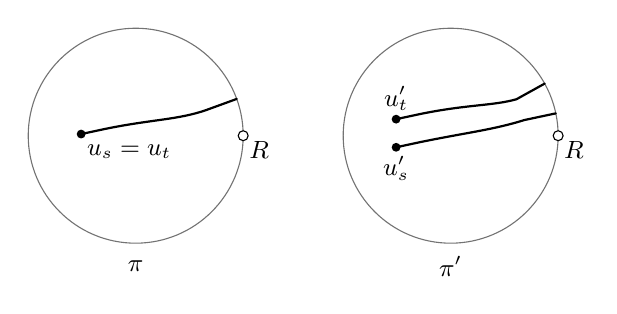
\begin{tikzpicture}[x=1.05cm,y=1.05cm,line cap=round,line join=round,
                    every node/.style={font=\small}]
  \begin{scope}
    \draw[black!55] (0,0) circle (1.30);
    \draw[thick] (-.66,.02) -- (-.38,.08)
       .. controls (.20,.20) and (.51,.19) .. (20:.91) -- (20:1.30);
    \fill (-.66,.02) circle (1.6pt);
    \node[below right,inner sep=2pt] at (-.66,-.04) {$u_s=u_t$};
    \filldraw[fill=white] (1.30,0) circle (1.8pt);
    \node[below right,inner sep=2pt] at (1.30,0) {$R$};
    \node at (0,-1.58) {$\pi$};
  \end{scope}
  \begin{scope}[xshift=4cm]
    \draw[black!55] (0,0) circle (1.30);
    \draw[thick] (-.66,.20) -- (-.38,.26)
       .. controls (.20,.38) and (.51,.36) .. (29:.91) -- (29:1.30);
    \fill (-.66,.20) circle (1.6pt);
    \node[above,inner sep=2pt] at (-.66,.23) {$u'_t$};
    \draw[thick] (-.66,-.14) -- (-.38,-.08)
       .. controls (.20,.04) and (.51,.07) .. (12:.91) -- (12:1.30);
    \fill (-.66,-.14) circle (1.6pt);
    \node[below,inner sep=2pt] at (-.66,-.17) {$u'_s$};
    \filldraw[fill=white] (1.30,0) circle (1.8pt);
    \node[below right,inner sep=2pt] at (1.30,0) {$R$};
    \node at (0,-1.58) {$\pi'$};
  \end{scope}
\end{tikzpicture}
\caption{Images of two disjoint vanishing disks in the base. Under $\pi$ the disks follow one path from their common critical value. Under $\pi'$ the same disks follow separate paths, in either prescribed order. The open circle marks the value of the reference fibre.}\label{fig:commonpaths}
\end{figure}

\subsection{The completed thimbles and the marked fibre}\label{sec:completedthimbles}

We calculate the morphisms in the completion stopped at the core of $F_0$. Here the core of a Liouville domain is the set of points which do not escape under positive Liouville flow. The core of its boundary hypersurface defines a stop in the contact boundary at infinity. There are many equivalent descriptions of a stopped category. For the present calculation we need one that preserves the individual disks: the order of their ends controls which Floer complex computes their morphisms.

\begin{proposition}\label{prop:diskhoms}
At a fixed Morse parameter one can equip the common-path thimbles with gradings and relative Pin structures so that their isomorphism classes are permuted by $G$. In the category stopped at the core of $F_0$ each disk has endomorphism cohomology $\C$ in degree zero. With the outgoing paths in increasing terminal-angle order, all backward morphism groups vanish. Distinct disks at a common critical value are mutually orthogonal in every degree.
\end{proposition}

We give the changes at the two ends of the fibration before making the Floer calculation. The first puts a radial product at infinity without changing the marked page. The second places all the thimbles in the half-plane chart used by Ganatra, Pardon and Shende.

\begin{proof}
We may standardize the Morse charts before choosing the paths in Lemma~\ref{lem:samedisks}. Here are details ensuring that this step respects the stabilizers. Average a local holomorphic chart, composed in each summand with the inverse tangent action, to linearize the stabilizer. The quadratic jet is a nondegenerate invariant complex quadratic form. In an invariant Hermitian metric its associated antilinear operator has antiunitary polar factor a real structure: in a unitary Takagi basis the operator is complex conjugation times a positive diagonal matrix. On the fixed real subspace the quadratic form is positive definite. Real orthonormal coordinates for that form give $q=\sum z_i^2$ with real orthogonal stabilizer action. To remove the terms $h$ of order at least three, solve $d(q+th)(v_t)=-h$. The gradient entries of $q+th$ are coordinates near zero, uniformly for $0\le t\le1$. In them $h$ is a sum of the entries times functions of order at least two, by integration along radii. Average the resulting holomorphic field and integrate on a smaller ball.

After removing the real pluriharmonic part of its quadratic Taylor polynomial, an invariant potential $P$ for the local Kähler form has positive Hermitian quadratic term. Let $P_0$ give the standard form, proportional to $|z|^2$. Replace $P$ by $P+t\chi(P_0-P)$ in each of the disjoint charts. Choose the radial cutoff $\chi$ equal to one near zero and zero outside the chart, with $|r\chi'|+|r^2\chi''|$ small by taking a long transition in $\log r$. Since $P_0-P=O(r^2)$ and $d(P_0-P)=O(r)$, the cutoff errors in the Levi form are smaller than the uniform positive lower bound of the convex combination. This gives a deformation through invariant primitives by adding $d^c(t\chi(P_0-P))$ to the fibrewise construction before the base-area addition. In the added base term use $\kappa b(|w|)\alpha_0$ with $b$ nondecreasing, zero on a disk containing the Morse charts and one on an outer annulus. This changes the primitive through nonnegative additions of base area, preserves the outward estimates and makes the \emph{total} form standard at each centre. On the product horizontal collar, $\alpha_R-\alpha_0=df$ with $f(R)=0$. Subtract $d(\nu f(\pi))$ using a fibre cutoff $\nu$ equal to one near the face and supported away from the disks. There the resulting product primitive is $\lambda_F+(1+\kappa b)\alpha_0$. The marked fibre retains its restricted primitive, and the compact vertical-face errors are bounded before increasing $\kappa$. In the separated fibration of Lemma~\ref{lem:samedisks} we now subtract $(\pi')^*((1+\kappa b)\alpha_0)$ to obtain the fibrewise primitive. This gives $\lambda_F$ on the horizontal collar. Near each Morse centre $b=0$ and the subtracted area is of type $(1,1)$ and vanishes at the centre, so the fibrewise form is Kähler on a smaller chart. On all radial ends $b=1$. The radial change of base coordinate $w\mapsto\sqrt{1+\kappa b(|w|)}\,w$ makes the exterior base primitive standard. We keep the old coordinate until the next calculation is finished.

On a short annulus $R_0\le r\le R$ trivialize in the radial direction by parallel transport for a separated presentation $\pi'$, with total primitive $\Lambda$. This follows each actual disk in its radial collar. Set $K=1+\kappa$ and $\Theta=\Lambda-K(\pi')^*\alpha_0$. Let $\zeta(r)$ be smooth and nondecreasing, equal to $r$ near $R_0$ and to $R$ near $R$. Write $j_s$ for the substitution of $\zeta_s(r)=(1-s)r+s\zeta(r)$ for $r$ in this trivialization. On the annulus replace $\Lambda$ by
\[
                         j_s^*\Theta+K(\pi')^*\alpha_0.
\]
The fibre form is constant in these radial coordinates and $d\Theta$ pairs the radial vector with each vertical vector to zero. If $a$ denotes the original horizontal area coefficient relative to $r\,dr\wedge d\theta$, the new coefficient is
\[
              K+\zeta_s'(r)\frac{\zeta_s(r)}{r}
                              \big(a(\zeta_s(r))-K\big).
\]
For the unsplit map $a-K$ is uniformly bounded independently of $K$; adding base area preserves the connection. Choose the annulus and cutoff first, then $K$ large enough for positivity there. For this fixed $K$, sufficiently small splitting times preserve strict positivity by smooth dependence of radial transport on the compact annulus. There are finitely many refinements. The tangential primitive at $r=R$ and the horizontal product collar stay fixed, including the corner rounding. The radial substitution takes each terminal collar into itself, where the primitive vanishes on the disk. Thus the disks remain Lagrangian with Legendrian ends. Identify the completed collars by boundary point and Liouville time. Exact Moser transport in the compact part then gives an exact isotopy of the disks with fixed cylindrical ends avoiding the stop, hence identical objects up to isomorphism \cite[Remark~2.30]{GPS}.

At $s=1$ continue the primitive as $\beta+p\,d\theta$, $p=Kr^2/2$, where $\beta$ is pulled back from the bundle on the outer circle. Attach the product fibre end as well. On the universal cover of the circle use the kernel of $d\beta$ for angular transport, starting at the reference fibre at $\theta=0$. Thus $d\beta=\omega_F$, and
\[
       \beta=\lambda_F+dG,\qquad
       G(\theta,x)=\int_0^\theta\beta(\partial_\vartheta)(\vartheta,x)\,d\vartheta .
\]
This follows by differentiating along the fibre, using $\beta|_{TF}=\lambda_F$ at $\theta=0$. The integral fixes the constant on every fibre component and is zero on the product fibre end. If $\mu$ is the monodromy, $k(x)=G(2\pi,x)$ satisfies $\mu^*\lambda_F-\lambda_F=dk$ and
$G(\theta+2\pi,x)=k(x)+G(\theta,\mu x)$. To flatten the primitive away from a short angular interval, choose $G_0=\rho(\theta)k(x)$ on one strip, with $\rho$ zero near zero and one near $2\pi$, extending by this same relation. Smoothness at the seam uses constancy of $\rho$ near both ends. Then $D=G_0-G$ descends to the circle bundle and has compact fibre support.

Change the primitive by $d(\chi_P(p)D)$, with $\chi_P$ zero up to a large $P$ and one beyond $2P$. The two-form is fixed. The tails of the geometric disks are products $V_i\times\{\theta_i\}\times[P,\infty)$ with $V_i$ compact exact vanishing spheres. To keep a disk cylindrical through the change, subtract the differential of an extension of the \emph{function} $\chi_P(p)D(\theta_i,x)$ on its tail, cut off in the fibre and in angle away from the marked ray. This preserves the primitive on the disk, also on the transition in $p$. For a zero-dimensional vanishing sphere the two restriction constants may differ. Outward Liouville flow identifies the resulting cylindrical representative with the usual cylindrization for the new uncorrected primitive \cite[\S7.2, (7.7)--(7.9)]{GPS}.

To check the stop under this identification, write the primitive as $p\,d\theta+\lambda_F+dg$ in angular transport coordinates. Its Liouville field satisfies $\dot p=p+\partial_\theta g$ and $\dot\theta=-\partial_p g$. All angular derivatives of the corrections are bounded on a fundamental strip. Take $P$ large so $\dot p\ge p/2$ in the region of change. Before it, outwardness at the original base boundary persists because $\partial_\theta G$ is independent of $p$. The fibre end is a product. These estimates give complete outward flows from a common compact carrier, whose conjugacy identifies the primitives strictly. On the reference ray $G(0,x)=G_0(0,x)=0$, all disk cutoffs vanish, $\dot\theta=0$, and the vertical field is exactly $Z_F$. Its core is invariant in both directions. The stop is therefore the same core of $F_0$. Applying the same conjugacy throughout the interpolation transports the cylindrical disks by an exact cylindrical isotopy. The calculation below can be made in the resulting flat model.

\medskip
\noindent\emph{A half-plane containing the outgoing paths.}
Write $0<\theta_1<\cdots<\theta_\mu$ for the small terminal angles. Choose $0<a<\theta_1$ and put the transition of $\rho$ strictly inside $(0,a)$. In the angular trivialization based backwards at $2\pi$, the primitive at large base radius is exactly $\lambda_F+p\,d\theta$ on a neighbourhood of $[a,2\pi]$. Indeed the fibre primitive after the transition on the original strip is $\mu^*\lambda_F$. The backwards trivialization removes this pullback and crosses the seam where the new potential is zero. It is important to put the positive-real stop at the \emph{upper} end of the right half-plane in \cite[\S8.6]{GPS}.

Let $f$ be an increasing circle diffeomorphism carrying $[-\pi/2,\pi/2]$ to $[a,2\pi]$ in this lift. The map $(p,\theta)\mapsto(p/f'(\theta),f(\theta))$ preserves $p\,d\theta$ and takes rays to rays. To place also the finite part of the half-plane in the exterior chart, first apply a compactly supported Hamiltonian translation. In Cartesian coordinates take $Cy\,\chi(y/T)\psi(x/T)$ with the sign translating by $+C$ along the real axis, with both cutoffs one on $[-1,1]$ and zero outside $[-2,2]$. Choose $C$ large compared with the inner radius of the chart times $\sqrt{\max f'}$. The time-one displacement is bounded by a constant times $C$, independently of $T$. For $T$ sufficiently large the half-disk of radius $T/2$ is translated by $+C$. Points outside it stay at large radius and change angle by $O(C/T)$, within the available angular margin. Composing with the polar map gives a proper embedding $j$ of the closed right half-plane into the chart. Its upper boundary end maps to the marked ray and all the thimble tails lie on the images of interior rays. The primitive difference is $j^*\alpha_0-\alpha_0=dh$ for a compactly supported function $h$, by compact Hamiltonian isotopy.

On a noncompact fibre a correction compactly supported in the base alone would not give the required Liouville embedding at total-space infinity. Extend $h\circ j^{-1}$ from the closed image to a smooth compactly supported function $h'$ of the target base, using a collar of its boundary. In the product fibre end subtract $d(\nu h'(\pi'))$, where $\nu$ is zero on a large compact fibre set and one past a larger level. The resulting difference on the product half-plane chart is the differential of $(1-\nu)h$, compactly supported in the total space. In fibre-end coordinates $I\alpha_F$ the added fibre covector is a multiple of $dI$, so evaluating the Liouville equation on the fibre Reeb field still gives $\dot I=I$. The change vanishes near a compact carrier with base radius above the support of $h'$ and fibre radius below the support of $\nu$. Fibre radial growth and the unchanged base growth beyond that support identify completions by their outward flows. The fibre cutoff can be placed beyond all the disks over the compact base support. Around their tails and the marked core the previous primitives and cylindrical identifications persist. For a finite fibre the product correction already has compact support.

\medskip
\noindent\emph{Floer cohomology.}
Each disk now has, outside a compact set, a compact exact fibre slice times a ray in this half-plane. Thus it is a thimble-like object of \cite[Definition~8.19]{GPS}. By full faithfulness in \cite[Proposition~8.20]{GPS}, its morphisms in the stopped category can be computed by moving the source in increasing terminal angle above the target and using ordinary Floer cohomology there. For $\theta_i>\theta_j$ the source is already above the target. The two disks lie over disjoint paths, and a sufficiently small positive pushoff at the source end still misses the target. The complex has no generators.

For a self-morphism move the path slightly to its left, rotating it by a small positive angle $\delta$ at its Morse centre and increasing its terminal angle. A normal strip along the path gives such a pushoff meeting the old path only at the centre. Transporting the vanishing sphere through these paths gives a positive thimble-like isotopy; its compact slice may vary from one path to the next. At the centre the two tangent planes in the standard quadratic chart are $\mathbb R^n$ and $e^{i\delta/2}\mathbb R^n$, after fixing the initial phase. The whole Floer complex therefore has one generator and zero differential. Its endomorphism cohomology is a nonzero unital graded algebra, so its one dimension lies in degree zero. Lemma~\ref{lem:samedisks} allows both orders at each common value. The two backward vanishings obtained this way concern the same original disks.

Finally start on the logarithmic torus with the square of its logarithmic volume form. A fan automorphism changes the volume by a determinant $\pm1$, so this square is invariant. Extend it along the invariant deformations used above: choose invariant compatible metrics and transport the squared determinant line along the interval, then extend on Liouville collars. For relative Pin data take the product real bundle with the fan representation on its fibre, with background its second Stiefel--Whitney class. Each contractible disk has a unique relative Pin class up to isomorphism. Its circle-valued squared phase has a lift, and a stabilizer element changes a lift by a constant integer. Finite order forces that integer to be zero. Taking one lift per orbit and transporting gives the asserted action on the isomorphism classes of the decorated disks in the initial presentation. Only the auxiliary calculations after separation required a choice of order within a common value.
\end{proof}

\subsection{Generation by the individual disks}\label{sec:diskgeneration}

The morphism calculation leaves open whether the disks generate. A Weinstein handle of middle index has a distinguished Lagrangian disk, its cocore, obtained by flowing the local unstable disk outwards. The handle-attachment theorem gives generators in terms of these cocores. We shall choose a Liouville primitive whose unstable manifolds are precisely the geometric disks used in Proposition~\ref{prop:diskhoms}. We work in the idempotent-complete derived partially wrapped category.

\begin{theorem}\label{thm:diskgeneration}
For the fixed Morse presentation of Proposition~\ref{prop:diskhoms}, the individually labelled common-path thimbles form a full exceptional collection, in increasing terminal-angle order, in the category stopped at the core of the marked regular fibre. The group permutes their isomorphism classes, and within each common critical value any ordering is allowed. The subcategory generated by the disks over a value with $l$ critical points is equivalent to $\mathrm{Perf}(\C)^l$.
\end{theorem}

\begin{proof}
Choose a separation by Lemma~\ref{lem:samedisks} and use the flat completion and cylindrical representatives in the preceding proof. We first prepare a regular region over which the fibration is a product, including a corridor to the marked ray. The connection on this region can have curvature initially.

\medskip
\noindent\emph{A product away from the vanishing paths.}
Enclose each path in a thin closed region formed by a disk about its starting point and a strip along the path widening to a small angular sector on its radial end. Take the regions disjoint from one another and from the marked direction at infinity. In a large base disk $B_R$ the closed middle $M$ left after deleting their interiors is a disk with corners disjoint from every path. Enlarge it slightly across its edges and beyond the outer circle, and smooth to obtain an open disk $V$ avoiding all the paths. Contract $V$ to $q_0=R$ on the marked ray by a smooth contraction $h_t$ fixing $q_0$. For a cutoff $\chi$ supported in $V$ and equal to one on a neighbourhood of $M$, put $k_s(w)=h_{s\chi(w)}(w)$, extended by the identity. Thus $k_s$ changes points only through regular values, fixes the paths with their neighbourhoods, and $k_1=q_0$ near $M$.

Let $\Lambda$ be the flat-end primitive, adapted to the individual disks, and $\Theta=\Lambda-\pi^*\alpha_0$, using the base coordinate in which the plane primitive is standard. On the product fibre end and in the product chart at $q_0$ we have $\Theta=\lambda_F$. Choose a nonnegative plane area form $\omega_b$ allowing zeros, zero on disks about the critical values and standard outside slightly larger disks disjoint from $\overline V$. Choose a primitive $\beta$ vanishing on the smaller disks and equal to $\alpha_0+c\,d\theta$ near infinity. Indeed the constant $2\pi c$ is the integral of $\omega_b-d\alpha_0$. After removing this period the remaining difference on the end is exact, as are the restrictions on the inner disks. Cutoffs of these exact corrections give the required primitive. At large $R$ its angular coefficient is positive.

On the pullback
\[
 E_s=\{(w,x):w\in B_R,\ \pi(x)=k_s(w)\},\qquad \pi_s(w,x)=w,
\]
take the primitive $\operatorname{pr}_E^*\Theta+\pi_s^*(\alpha_0+A\beta)$ and truncate in the product fibre end. The pullback is smooth even at $s=1$: on the changed region $\pi$ is a submersion, while near each critical point $k_s$ is the identity. Horizontal lifting along $s\mapsto k_s(w)$ identifies the truncated family, by the identity near the paths and in product coordinates near the page. A small neighbourhood of $q_0$ stays in its product chart for all $s$ by compactness.

The new horizontal lift of $v$ is $(v,\widetilde{dk_s(v)})$. Its horizontal area form is $d\alpha_0+A\omega_b+k_s^*((d\Theta)_{\rm hor})$. On the changed compact part the last term is bounded independently of $A$ and on the fibre end it vanishes. Thus a single large $A$ gives positive area even when $dk_s$ drops rank. Elsewhere one has added nonnegative base area, leaving the standard critical charts intact. On the horizontal face the fibre field is outward. On the vertical face the primitive on the angular lift has the positive summand $A\beta(\partial_\theta)$ and the remaining terms are uniformly bounded. At $s=0$ first turn on $A\beta$; its angular contribution at $R$ is nonnegative throughout. The disks stay Lagrangian and conical, since the added base primitive vanishes on the radial tails. The far radial momentum is now $p+A(p+c)$ for $p=|w|^2/2$. This increasing change of radial coordinate preserves the page direction and fibre core.

The interpolation in $k_s$ keeps the disk neighbourhoods, the page germ and the horizontal product collar fixed under these identifications. Relative contact isotopy on the remainder of the compact boundary, followed by compact Moser transport, identifies the completed pairs and their disks. Here the contact conformal factor is absorbed by translation in Liouville time on the collars before applying Moser, and the transports may be fixed on the unchanged neighbourhoods. At the endpoint freeze radial transport on a short outer annulus as in Proposition~\ref{prop:diskhoms}, resampling the term from $\Theta$ and retaining $\alpha_0+A\beta$. The horizontal curvature and its resampled error are uniformly bounded there independently of $A$, since base addition preserves the connection. Choose $A$ at the outset to dominate this bound as well. The outer middle and its edge collars are already products, since $k_1$ is constant there on an open neighbourhood. In that part freezing preserves $\lambda_F$ and the product extends over the infinite middle. On each disk the radial substitution and collar identification again preserve the cylindrical representative.

\medskip
\noindent\emph{A Weinstein primitive adapted to the disks.}
Straighten the separated paths to radial rays $r e^{i\theta_i}$, $r\ge1$, moving their caps into $r>3/4$ and keeping their angles at infinity. This uses a compactly supported orientation-preserving base diffeomorphism. Prescribe translations and rotations on path tubes near their starts and the identity near an outer circle. The complementary regions, slit along those tubes, are disks. Their boundary identifications extend over collars and then across the disks. Such a postcomposition preserves fibres and horizontal transport on corresponding paths. Rotations at the centres are absorbed by unitary scalar changes in the quadratic charts. The disk $r\le2/3$ and a corridor about the entire marked ray now have the same product fibre. The projection, again denoted by $\pi$, is $c_i+\sum_jz_j^2$ in a standard chart, with $c_i=e^{i\theta_i}$.

Subtract a base one-form equal to the base part of the total primitive on a slightly smaller product disk and corridor, equal to its base part at infinity, and zero near the centres. These prescriptions agree on overlaps and extend by cutoffs. Write $\vartheta$ for the difference. On a smaller Morse ball a local exact change gives $\vartheta=\lambda_{\rm std}=\sum_j(x_jdy_j-y_jdx_j)/2$. Choose a generic Weinstein fibre primitive $\lambda_F^W=\lambda_F+dg$ with $g$ compactly supported. Indeed the strictly plurisubharmonic fibre exhaustion has no critical points beyond a compact level. Perturb it to Morse on the interior, keeping the regular collar, and pull the new forms back by compactly supported exact Moser transport. The resulting primitive differs by the differential of a compactly supported function. A finite fibre needs no perturbation. Add $d(\chi g)$ using a base cutoff equal to one on $r\le0.55$ and on a smaller marked corridor and supported inside the product. The complete page ribbon follows the change of its restricted primitive, away from the links of the disks at infinity \cite[Example~3.11]{GPS}.

The restriction of $\vartheta$ to each disk is exact since base area restricts to zero and the disk is contractible. It already vanishes near the centre, where the disk is a rotated real plane. Normalize its primitive to zero there and subtract the differential of a tubular extension cut off near the disk. Use disjoint tubes away from the smaller product disk and marked corridor. On a radial tail the fibre slice is compact and the gauge can be chosen independent of $p$, with compact fibre support. This allows both restriction constants on a zero-dimensional slice. We have obtained
\[
  \vartheta|_{TD_i}=0,\qquad \vartheta=\lambda_{\rm std}
                     \quad\text{near each critical point}.
\]
On the smaller product disk and the marked corridor, $\vartheta=\lambda_F^W$. Use $\Lambda_K=\vartheta+K\pi^*\alpha_0$ for large $K$. To deform to it, first add the large base term, then interpolate the subtractions. On regular compact sets the curvature errors and angular covectors are bounded independently of $K$. In the Morse charts the subtracted base form was zero. The connection and fibre forms are preserved. At large base radius the angular gauges have bounded derivatives with compact fibre support, giving strictly positive radial growth. The product fibre end still has $\dot I=I$ in its symplectization coordinate. These estimates give complete convex enlargements. On the far disk collars the initial and final adapted primitives vanish along disk tangents, as do all base forms along radial tangents. The disks thus persist as exact cylindrical objects during this deformation.

\medskip
\noindent\emph{The ascending manifolds.}
Set $H=|\pi|^2$ and $\iota_{Z_K}d\Lambda_K=\Lambda_K$. On compact regular subsets with $r$ bounded away from zero the projected field tends to $w/2$ by the horizontal two-plane formula. Hence $dH(Z_K)>0$ there for large $K$. The product fibre end gives the same bound for bounded base radii away from zero. At base infinity $\dot p=p+O(1/K)$ in the flat angular charts. Close to a critical point write $w=c+q(z)$ with $q=\sum_j z_j^2$, and put $a=4|z|^2$. On the standard horizontal complex line $d\pi$ is conformal of scale $\sqrt a$. The standard Liouville field is half the radial field on the $z$-coordinates, so its projection is $q$. The new projection is the average of $q$ and $w/2$ with weights $1$ and $Ka$. Thus
\[
                  dH(Z_K)=
           \frac{2\operatorname{Re}(\bar w q)+Ka|w|^2}{1+Ka}.
\]
Here $|q|\le|z|^2$ and $|w|$ is bounded away from zero. For fixed large $K$ the right side is bounded below by a positive multiple of $|z|^2$ in a small ball off its centre. At the centre $Z_K=0$ and $H$ has index $n=\dim_\C X$ by its quadratic part $2\operatorname{Re}(\bar c q)$. Rotate to $c=1$ in this calculation. The added linear covector is $K\,d\operatorname{Im}q/2$, so the linearized field has eigenvalues $1/2+K$ on the real plane and $1/2-K$ on the imaginary plane. The former is tangent to the outgoing disk.

To get a proper Weinstein function, choose a nonnegative radial function $h_\infty(I)$ on the product fibre end, zero on a large compact fibre part, nondecreasing and eventually linear and unbounded. Choose the fibre Lyapunov function $h_0\ge0$ for $\lambda_F^W$ to have critical values below $1/100$, to agree with $h_\infty$ far out, and to be uniformly close to it. Indeed one can add $\varepsilon$ times a shifted Morse Lyapunov function to $h_\infty$ on the compact region, extend increasingly along the collar until $h_\infty'>0$, and cut off the summand where this derivative is bounded below. With a radial base cutoff $\rho$ equal to one near zero and zero for $r\ge1/3$, put
\[
                         \Phi=H+h_\infty+\rho(r)(h_0-h_\infty).
\]
This is proper and near zero is a product Weinstein function. On the transition its fibre derivative is a convex combination of nonnegative derivatives, and the cutoff error is dominated by $dH(Z_K)=r^2$ there for small $\varepsilon$. Elsewhere $dh_\infty(Z_K)\ge0$ by the product fibre-end equation. At the centres the preceding quadratic bound gives the gradient-like inequality since both $dH$ and $Z_K$ are $O(|z|)$. The critical points besides the centres are the fibre critical points over zero, all of index at most $n-1$. The centres all have value one, so no trajectory connects two distinct centres.

The sublevel $\Phi\le1/5$ lies inside $r<0.55$ with primitive $\lambda_F^W+K\alpha_0$. Its completion is the entire stabilization $F\times\C$: the same product exhaustion extends throughout that product, with no critical values above $1/5$, so backward flow from outside reaches the level. Truncate $F$ above its core and below the start of $h_\infty$. The product of this truncation with $w=\sqrt{1/5}$ is the incoming page ribbon. On the whole marked corridor $Z_K=(Z_F^W,w/2)$, and forward flow preserves the reference direction and identifies the incoming with the original stopped core. Every point in that corridor with nonzero base radius flows outward at its fixed angle. The stable attaching spheres of the critical points miss the corridor.

The elementary Weinstein cobordism above this sublevel is given by disjoint critical handles on the free part of the incoming boundary \cite[\S6.3, Lemma~6.6]{GirPar}. Each prescribed $D_i$ is its completed unstable disk. Since the path is radial, $\Lambda_K|_{TD_i}=0$ and $Z_K$ is tangent everywhere. The real disk at the critical point has the expanding tangent plane, hence is the local unstable manifold by uniqueness. Every point of $D_i$ flows backwards into that germ, since each bounded segment is compact and $dH(Z_K)$ has a positive minimum on closed segments away from the centre. Conversely its forward saturation lies in the disk. One may keep this Lagrangian germ in the relative handle normal form: in the chart the Darboux interpolation for the added area uses the primitive $K(q_R\,dq_I-q_I\,dq_R)/2$, $q=q_R+iq_I$, which vanishes on the real plane. The Moser field is tangent there and has zero linearization. In the resulting coordinates the given and standard primitives restrict to zero on the plane, so a primitive of their exact difference can be set to zero there. The cutoff in the relative normal form preserves this restriction. Flow continues the identified cocore through the regular levels with the disk's transported grading.

\medskip
\noindent\emph{The retained page.}
The incoming stopped product is represented by the sector $P=F\times\C_{\operatorname{Re}\ge0}$ in \cite[(3.3)]{GPS}. A sufficiently small ribbon for the page core misses all attaching spheres by the corridor construction. Write $\mathcal L$ for their union and $P'$ for the attached sector. Under the attachment functor $\mathcal W(P,\mathcal L)\to\mathcal W(P')$ a small linking disk at a component of an attaching sphere maps to its handle cocore up to a grading shift. Both disks are images of a cotangent fibre of the handle overlap \cite[\S11.3]{GPS}. The disjoint charts allow all the identifications simultaneously. In dimension one an attaching sphere is $S^0$. The two overlap fibres on the handle side are cotangent fibres over the same interval and both give the one cocore up to shift. The source is generated by the linking disks of $\mathcal L$ by \cite[Theorem~1.16]{GPS}.

The original fibre page is still a stop after the attachment. It therefore contributes its own linking disks to the generation theorem, and we must see where these disks come from. For this purpose use the Weinstein convexification of the target with its original page stop. The incoming stabilization has handles only of index less than $n$. The generic fibre core is a mostly Legendrian stop, and the new cocores avoid it at infinity. By \cite[Theorem~1.13]{GPS} the target is generated by the new cocores and linking disks to the smooth Legendrian part of the original page core. These latter disks are already in the image of the attachment functor. Choose each in the incoming product corridor near its page and away from $\mathcal L$. The sector-to-ribbon and ribbon-to-core comparisons with the disjoint extra stop give an object of $\mathcal W(P,\mathcal L)$. Its page neighbourhood survives attachment, so the image is the corresponding outgoing linking disk, as in \cite[(9.6)]{GPS}. Thus the images of the attaching linking disks generate the target in the perfect envelope. They are exactly the cocores identified with our thimbles. Proposition~\ref{prop:diskhoms} supplies their morphism groups and the action on the initial collection. The endomorphism algebra of the sum of $l$ mutually orthogonal exceptional objects has cohomology $\C^l$ concentrated in degree zero, giving $\mathrm{Perf}(\C)^l$ as asserted.
\end{proof}


\section{From thimbles to perfect complexes}\label{sec:coherenttransport}

The group acts on a thimble by moving its critical point and preserving its path in the base. On a coherent sheaf it acts by pullback. To compare these actions one must keep track of the regular fibre throughout the passage to the cotangent bundle. There the group acts by diffeomorphisms of a real torus, whose action on sheaves can be read off directly.

Let $M=N^\vee$, let $T_a=M_{\mathbb R}/2\pi M$ be the angle torus, and, for a cone $\sigma\in\Sigma$, let $T_\sigma$ be the annihilator in $T_a$ of $N\cap\operatorname{span}_{\mathbb R}\sigma$. Use an invariant norm on $N_{\mathbb R}$ to write $S^*T_a=T_a\times S(N_{\mathbb R})$. The two conic links that will occur are
\[
 \Lambda_\pm^\infty
    =\bigcup_{0\ne\sigma\in\Sigma}T_\sigma\times
                       \big((\pm\sigma)\cap S(N_{\mathbb R})\big).
\]
The corresponding closed conic sets in $T^*T_a$, with the zero section included, are denoted by $\Lambda_\pm$. A fan automorphism $g$ acts on angles by $h_g=(g^{-1})^\vee$ and on covectors by $g$. Its cotangent lift preserves both links. We use the primitive $\langle p,d\theta\rangle$.

\subsection{Following the marked fibre to the conic link}
A compact Liouville hypersurface in a contact boundary is sometimes called a ribbon. When we move a ribbon $j:F\hookrightarrow\partial Y$, we record its intrinsic primitive $\mu$ and a positive function $b$ on the boundary such that $j^*(b\alpha)=\mu$, where $\alpha$ is the ambient boundary form. This permits a change of radial section in the completion. It also specifies which core is the stop.

\begin{lemma}\label{lem:equivariantlink}
In positive dimension the completed pair of Proposition~\ref{prop:compactpair}, at the chosen $G$-fixed Morse parameter, is joined by deformations of compact Liouville pairs and strict identifications of completions to a cotangent disk of $T_a$ whose marked core is $\Lambda_+^\infty$. Each map and family commutes with $G$. The squared logarithmic grading continues to the vertical cotangent grading. One can use the same real background bundle for the relative Pin structures throughout.
\end{lemma}

\begin{proof}
The straight cutoff homotopy of Proposition~\ref{prop:compactpair} is a deformation of compact pairs fixed near $F_0$. In particular we may start with the ray polynomial $W=t\sum_{v}z^v$, $t>0$, where $v$ runs over the primitive ray generators. We use the geometric comparison of Fang, Hu, Sun and Zhou \cite{FHSZ}. We give the choices needed for a finite group, since a quadratic form given by declaring a lattice basis orthonormal need not be invariant.

Take $\Phi$ constructed in the proof of \eqref{eq:cycledual}, with homogeneous end $\phi_\infty$. There take the norm to be invariant and average the small smooth approximations. This preserves their $C^2$ bounds, the positive Hessian lower bound, the strict facet inequalities and the agreement with a homogeneous end. In particular the gradient on an entire facet of the polar polytope lies in the interior of the union of maximal cones containing its ray. These are the fixed-potential hypotheses of \cite[Appendix D, condition D.9, and \S T.16]{FHSZ}. Strong convexity and proper quadratic growth make $d\phi_\infty$ a homeomorphism with smooth inverse off zero. Indeed its value $p$ is attained at the unique minimum of $\phi_\infty(u)-\langle p,u\rangle$, and the Hessian at a nonzero minimum is invertible.

Use the normalized family $f_s$ of \cite[\S M.1, M.6--M.7]{FHSZ}. At $s=0$ it is $e^{-\beta}\sum_v z^v=W/R$, with $R=t e^\beta$. At $s=1$ the level $H=f_1^{-1}(1)$ is the tailored hypersurface. The cutoff of each monomial compares its weight with those of all the other exponents, using the same scalar functions for every pair. The height is one at each vertex and zero at the constant. The remaining cutoff depends on $\sum_v |e^{-\beta}z^v|^2$. Thus relabelling the rays preserves the functions $f_s$ themselves, including their phases.

Choose $D_-$ above the fibre truncation threshold of \cite[Q.2]{FHSZ}, then $D\ge\max(D_-+1,D_0)$ with $D_0$ from \cite[U.31]{FHSZ}. Write
\[
        A_-=D_-^2\beta^2/2,\qquad A=D^2\beta^2/2,\qquad K=\kappa R^2.
\]
First take $\beta$ sufficiently large for these fixed radii, with $R$ beyond the image of the common compact critical-point bound of Proposition~\ref{prop:compactpair}. Take $A_-$ above the $\Phi$-values on that compact set. The reference fibre then has the allowed truncation $L'=A_-$ by the outwardness estimate of \cite[Q.2]{FHSZ}. Choose the exterior horizontal level of Proposition~\ref{prop:compactpair} afterwards, then $\kappa$ large enough for both constructions. Write $m_\delta$ for a smooth maximum agreeing with the larger argument outside a $\delta$-neighbourhood of equality. With $\delta<A-A_-$ sufficiently small the pairs of \cite[Q.15--Q.16, Q.21, Q.23--Q.27 and Q.35]{FHSZ} are
\begin{align*}
 Y_s&=\{m_\delta(\Phi-A,e^{2\beta}(|f_s|^2-1))\le0\},\\
 F_s^-&=\{f_s=1,\ \Phi\le A_-\},\qquad
 \lambda_s=\lambda_\Phi+K f_s^*\alpha_0,\qquad
 \lambda_\Phi=-d\Phi\circ J .
\end{align*}
The indicated results give smooth fibres of this compact family, an outward ambient field, and the embedded hypersurfaces with primitive $\lambda_\Phi|_{F_s^-}$. All defining functions are invariant. Lifts of $\partial_s$ tangent to the ambient boundary, the hypersurfaces and their frontiers exist in family charts. Their defining tangency and time-component conditions are affine, so a partition of unity and averaging give a single invariant lift. Its flow trivializes the compact pairs, including the boundaries.

At $s=0$ the primitive equals $\lambda_\Phi+\kappa W^*\alpha_0$. The two boundary germs on the entire truncated fibre coincide, since its vertical face is $|W|=R$ in both constructions. The rounding may be taken small enough to include the common compact critical-point bound in the interior of $Y_0$. The exhaustion $\Phi+\kappa |W|^2/4$ increases strictly along the complete ambient field outside that compact set, as in Proposition~\ref{prop:compactpair}. A negative trajectory staying outside $Y_0$ would remain in a compact sublevel on which the rate of increase has a positive minimum. Thus every such trajectory reaches the boundary. The two completions identify strictly with the same torus, with the same marked hypersurface.

It remains to carry the hypersurface to a boundary on which its core has an explicit equation. Set $D_\beta=\{\Phi\le A\}$ and
\[
 \Gamma=\bigcup_{0\ne\sigma\in\Sigma}
 \{(u,\theta):d\phi_\infty(u)\in\sigma\setminus\{0\},\
                                              \theta\in T_\sigma\}.
\]
The fixed-potential core calculation of \cite[\S T.16, T.115--T.116]{FHSZ} identifies the core of $F_1^-$ with $H\cap\Gamma$. The inclusion of $Y_1$ in $D_\beta$ identifies their completions strictly for the primitive $\lambda_\Phi+Kf_1^*\alpha_0$ by \cite[Q.59]{FHSZ}. To transfer the embedded ribbon through this identification and then remove the base area, put $\lambda(k)=\lambda_\Phi+kf_1^*\alpha_0$, $0\le k\le K$. By \cite[U.31, U.34--U.41, U.46--U.54]{FHSZ}, the $\lambda(k)$-Liouville trajectories from a common neighbourhood of $H\cap\Gamma$ in $H$ hit $\partial D_\beta$ transversely. The first-hit maps $\pi_k$ embed that neighbourhood after shrinking and carry the core onto $\Gamma\cap\partial D_\beta$. The times $\tau_k$ and maps commute with $G$ by uniqueness of flow. The neighbourhood may be intersected with its finitely many translates. A scalar cutoff of the field used to extend its flow may be averaged after requiring it to be one on the union of the retained compact trajectory bands.

The negative intrinsic Liouville flow $a_T$ of the fibre takes all of $F_1^-$ into this neighbourhood for a common finite $T$, preserving its core. This follows by compactness from the description of the core as the intersection of the nested negative images. In dimension one the fibre is a finite set and $a_T$ is the identity. On the fixed compact ribbon carrier put $j_k=\pi_k a_T$ and $\mu_T=e^{-T}\lambda_\Phi|_{F_1^-}$. Then
\[
                     j_k^*\lambda(k)=e^{\tau_k\circ a_T}\mu_T .
\]
Indeed a variable flow time contributes a multiple of the Liouville vector field, on which the primitive vanishes. Extend $-\tau_k\circ a_T$ as a smooth function from the moving embedded ribbon to the boundary family, also along its frontier. Average the extension and exponentiate. This gives the required witness $b_k$ on the whole boundary. At $k=K$ a strict change of section with radial shift $s$ pulls the outgoing boundary form back to $e^{-s}$ times the incoming one. On our ribbon $s=-\tau_K\circ a_T$ by \cite[U.55--U.57, V.1--V.13]{FHSZ}. Thus its transferred witness agrees with $b_K$ on the ribbon. Interpolating their logarithms gives a deformation fixing the embedded ribbon and its intrinsic form. We may now decrease $k$ to zero.

The Legendre map $(u,\theta)\mapsto(\theta,d\Phi(u))$ is strict at $k=0$. The boundary lies on the homogeneous end, so radial normalization $p\mapsto p/\|p\|$ carries its intersection with $\Gamma$ onto the whole link $\Lambda_+^\infty$. The boundary form is divided by $\|p\|$ and the witness is multiplied by this same norm. Invariance of $\Phi$ identifies the group action with the cotangent lift of $h_g$.

Finally consider the grading. The squared logarithmic volume is invariant since each lattice determinant has square one. The forms $d\lambda_\Phi+kf_s^*d\alpha_0$ give a symplectic rectangle on the required carriers by the Poisson bracket estimate of \cite[Lemma~O.5]{FHSZ}. Take compatible complex structures by polar decomposition using the invariant logarithmic Kähler metric. On $k=0$, and also on $s=0$ by holomorphicity, this gives the logarithmic complex structure. Parallel transport the squared volume in $k$ by the projected connection $\nabla_k\sigma=P_k\partial_k\sigma$, where $P_k$ is orthogonal projection to the varying canonical square. It is constant on the holomorphic edge. This gives a grading along the top of the rectangle returning to the logarithmic one at $(1,0)$. For the earlier compact perturbation the same construction uses the straight contraction to $W$, the bracket bound in Section~\ref{sec:compactmirror}, and continuation along the interval of flattened primitives. Strict inclusions agree on their common interior, and the grading extends along invariant radial collars. To identify the terminal class, let $B$ be the invariant inner product on $M_{\mathbb R}$ and $H_\Phi=B^{-1}\operatorname{Hess}\Phi$. In a $B$-orthonormal frame the complex coframes
\[
         ((1-l)I+lH_\Phi)\,du+i\,d\theta,\qquad 0\le l\le1 ,
\]
are compatible with $d\lambda_\Phi$, as diagonalization of the positive $H_\Phi$ shows. Their invariant squared determinants join the log grading and the pullback of the vertical cotangent grading. The product real bundle with fibre $N_{\mathbb R}$ and diagonal $G$-action extends across all changes of carrier. At the cotangent end fibre translation identifies it equivariantly with the vertical tangent bundle, as required for the polarized relative Pin convention.
\end{proof}

\subsection{Transport with the group action}

We next explain how to use such a family to follow an individual brane. The point requiring care is that Moser transport of the ambient manifolds may move the intrinsic core inside a hypersurface. A neighbourhood of the whole hypersurface in the contact boundary permits a comparison even in this case.

\begin{lemma}\label{lem:geometrictransport}
Suppose a finite group acts fibrewise on a smooth compact interval family of Liouville pairs with boundary forms $\alpha_t$, embedded hypersurfaces $j_t:F_t\hookrightarrow\partial Y_t$, and invariant positive functions $b_t$ satisfying $j_t^*(b_t\alpha_t)=\mu_t$ for the intrinsic Liouville primitives $\mu_t$. Give the family a compatible grading and a background bundle with the specified group identifications. There is an equivalence of the categories stopped at the two endpoint cores whose induced bijection on isomorphism classes of geometric branes commutes with each element of the group. It extends to an equivalence of their perfect envelopes.
\end{lemma}

\begin{proof}
Trivialize the compact carriers by an averaged interval lift, and attach invariant cylindrical ends. On the fixed completion with forms $\lambda_t$ solve
\[
                   \iota_{V_t}d\lambda_t=-\dot\lambda_t .
\]
On the cylindrical end $\lambda_t=e^\ell\alpha_t$. The defining equation is homogeneous, so both components of $V_t$ in boundary and logarithmic radial coordinates are bounded. Its flow exists over the interval and commutes with the group. Evaluation against $\partial_\ell$ gives $\lambda_t(V_t)=0$ on the end, so Cartan's formula makes the primitive difference compactly supported and exact. We now have one contact boundary carrying the moving ribbons and their transported witnesses.

At a ribbon the Reeb vector of $b_t\alpha_t$ is transverse since the restriction of its differential to the hypersurface is symplectic. A short Reeb thickening $A_t$ therefore has coordinates $|z|\le\delta$, $x\in F_t$, with form $dz+\mu_t$. A short extension at the frontier and compactness allow one width on a small interval. This construction is invariant. The contact vector field $z\partial_z+Z_{\mu_t}$ points out at the faces. Its negative flow shrinks the thickening to sets whose intersection is the core of $F_t$ at $z=0$. The contact field extends over a collar by extending and averaging its contact Hamiltonian. The stop-forgetting functor from the thickening to the core is a quasi-equivalence \cite[\S3.2, Lemmas~3.5--3.6, Corollary~3.9]{GPS}. Indeed every finite inward shrink induces an equivalence, and morphisms at the intersection are the filtered direct limit of the wrapped Floer cohomology groups along stop-forgetting. The asymptotic boundary of each geometric brane disjoint from the core is compact and misses a finite shrink, giving essential surjectivity. This argument includes a zero-dimensional $F_t$.

For two nearby times write $A,A'$ for the thickenings. Extend an invariant inward contact field for $A$ across its frontier. Strict inwardness persists on the nearby frontier of $A'$; one may use the same small rounding of the product corners before making this choice. Fix a small positive flow time $\epsilon$. For $A'$ sufficiently close to $A$, the inward flow $\psi$ satisfies
\[
     \psi^{3\epsilon}(A')\ \subset\ \psi^{2\epsilon}(A)\
            \subset\ \psi^\epsilon(A')\ \subset\ A .
\]
The inclusions follow from the positive collar margins at $A'=A$ and compactness. Forget stops from right to left. The first two arrows composed and the last two composed are inward-shrink equivalences. The two-out-of-six property for equivalences gives equivalences for each arrow. The shrink from $A'$ to $\psi^\epsilon(A')$ completes the comparison. A finite subdivision of the parameter interval suffices by compactness.

Each forgetful functor carries an allowed geometric brane to the very same decorated brane in the target. Hence on geometric isomorphism classes its bijection and the inverse bijection commute with the individual symmetries. The ambient identifications act on geometric branes by transport. The paths of differentials lift to the grading cover from their given initial lifts, equivariantly by uniqueness. The specified identifications of the real background bundle transport the relative Pin structures. Thus these conclusions hold for decorated objects. The construction only uses the action of each geometric symmetry on isomorphism classes in the ordinary category, which can be computed by pushing the Floer data forward and comparing choices. Passing to twisted complexes and summands gives the last assertion.
\end{proof}

\subsection{Covariance at the cotangent endpoint}
Let $f_g:X\to X$ denote the toric automorphism with lattice map $g$. On the cotangent side $H_g$ denotes the lift of $h_g$. There is a covariant equivalence
\begin{equation}\label{eq:coherentendpoint}
  \mathcal E:\mathrm{Perf}\,\mathcal W(T^*T_a,\Lambda_+^\infty)
                          \longrightarrow \mathrm{Perf}(X)
\end{equation}
with $\mathcal E((H_g)_*L)\simeq(f_{g^{-1}})^*\mathcal E(L)$ for each brane $L$. Here is the direction of each functor. Cotangent inversion $I:(\theta,p)\mapsto(-\theta,-p)$ preserves the primitive and takes the positive link to the negative link. It commutes with the $H_g$, including on the vertical polarization. The latter fixes the graded lift: in an invariant frame the group preserves the constant phase lift of the vertical plane. Equivalently two genuine lifts of this finite group differing by deck translations on the connected ambient Grassmann bundle differ by a homomorphism to $\mathbb Z$, hence coincide.

Write $\mathcal S=\mathrm{Sh}_{\Lambda_-}(T_a)^c$ for the compact objects of the unbounded category of complex sheaves with the indicated microsupport. The link is closed, subanalytic and isotropic, since the finite conormal pieces lie over the annihilator subtori. Microlocal Morse theory gives an equivalence
\[
 P:\big(\mathrm{Perf}\,\mathcal W(T^*T_a,\Lambda_-^\infty)\big)^{\mathrm{op}}
                       \longrightarrow \mathcal S .
\]
For an analytic diffeomorphism of the base, the symplectic action here corresponds to the left adjoint of restriction on sheaves \cite[Theorem~1.1 and Proposition~1.3]{GPSmicro}. Thus it acts by $(h_g)_!$. We use complex coefficients in the strata and localization construction of that equivalence, as in \cite[Theorem~5.1]{FZ}. In the normalization of \eqref{eq:cycledual}, the coherent--constructible correspondence $\kappa:\mathrm{Perf}(X)\to\mathcal S$ takes toric pullback by a fan isomorphism $f$ to pushforward by the dual torus map $f_N^\vee$ \cite[\S9, (9.14), Remark~9.3 and Proposition~9.4]{Kuw}. For $f=f_{g^{-1}}$ this dual map is exactly $h_g$. We identify the two presentations of the angle torus by $\theta\mapsto\theta/(2\pi)$, scaling covectors inversely. Finally derived duality $D_X=\mathrm{R}\mathcal Hom_X(-,\mathcal O_X)$ is involutive on perfect complexes and commutes with pullback by an isomorphism. The composite
\[
                      D_X\circ(\kappa^{-1}P)^{\mathrm{op}}\circ I_*
\]
has the covariance and the action asserted in \eqref{eq:coherentendpoint}.

\begin{theorem}\label{thm:coherentcollection}
Let $X$ be a smooth projective complex toric Fano variety and let $G$ preserve its fan. There is a $G$-fixed semisimple parameter as in Proposition~\ref{thm:main} and a full exceptional collection of perfect complexes $(E_s)$ on $X$ indexed by its primitive idempotents such that
\[
                 (f_{g^{-1}})^* E_s\simeq E_{gs}.
\]
The collection may be ordered by the common paths of the distinct Euler values, in increasing terminal-angle order. The subcategory for a value $u$ of multiplicity $m$ is equivalent to $\mathrm{Perf}(\C)^m$. Its individual objects $E_s$ with $u_s=u$ can be taken in any order. The same collection works for all subgroups of the chosen group.
\end{theorem}

\begin{proof}
For a point take its structure sheaf. Otherwise apply Section~\ref{sec:compactmirror} to the invariant Morse parameter constructed in Section~\ref{sec:exist}. Proposition~\ref{prop:cluster} identifies the critical points of the retained cluster with the individual idempotents and their values with the Euler coordinates. Choose one path for each distinct value as in Lemma~\ref{lem:samedisks}. Give the resulting thimbles the brane data of Proposition~\ref{prop:diskhoms} using the product background of Lemma~\ref{lem:equivariantlink}. The invariant local changes used to make the disks cylindrical are deformations with the same far ribbon. Apply Lemma~\ref{lem:geometrictransport} along them in reverse, then along the deformation of Proposition~\ref{prop:compactpair} and that of Lemma~\ref{lem:equivariantlink}. Strict identifications at their junctions carry each brane by the graded map itself. At the endpoint use \eqref{eq:coherentendpoint}. The images of the actual disks now satisfy the displayed pullback formula.

The composite is an exact equivalence after passing to perfect envelopes. Theorem~\ref{thm:diskgeneration} gives fullness, and Proposition~\ref{prop:diskhoms} gives exceptionality, the backward vanishings and both vanishings at a tied value. Since $X$ is smooth, $\mathrm{Perf}(X)=D^b\mathrm{Coh}(X)$. The mutually orthogonal exceptional objects over $u$ generate the claimed product category, with admissible inclusion by the evaluation projections for exceptional objects on a proper variety. Restricting the pullback identity gives the assertion for subgroups.
\end{proof}

One may choose $G=\mathrm{Aut}(N,\Sigma)$ at the outset. A torus translation fixes each exceptional isomorphism class by rigidity (Section~\ref{sec:fieldmodels}). Thus finite groups normalizing the dense torus act on this collection through their fan projection. This gives the collection asked for in the geometric Merkurjev--Panin question in the smooth projective Fano case, in the ordinary derived category \cite[Introduction]{EHLZ}. The theorem specifies perfect complexes. Identifying their individual classes with a prescribed calibrated Gamma basis involves a further comparison: equivariance alone permits a change of integral basis. This is the purpose of Proposition~\ref{prop:ordinarymarking}. Proposition~\ref{prop:stabilizers} supplies linearizations on the individual fan stabilizers.

\section{Continuing an individual Gamma marking}\label{sec:markedpaths}

Let $\mathcal C_0$ denote the mirror category of Theorem~\ref{thm:diskgeneration}, with perfect envelopes understood, and write $D_s$ for its geometric disks. Theorem~\ref{thm:coherentcollection} gives an equivalence $U:\mathcal C_0\to\mathrm{Perf}(X)$ which describes their symmetries. We seek an ordinary equivalence on $\mathcal C_0^{\mathrm{op}}$ computing their individual classes. Taking the opposite reverses the order of the collection. As in Proposition~\ref{prop:ordinarymarking}, we will compare it with $D_X U$ on this same source.

\subsection{A regular ray potential}
For independent ray coefficients $c=(c_i)\in(\C^*)^m$ write $W_c=\sum_i c_i x^{v_i}$. There are two coefficient tuples of interest. The tuple $*=(t,\ldots,t)$ preserves the fan group and supplies the end of the compact perturbation. A second positive tuple $a$ lies in the actual small chart of \cite[\S3.1]{FZ} and has distinct Morse values. We explain both its existence and the connection between the charts.

The incidence $\sum c_i x^{v_i} v_i=0$ is smooth of dimension $m$ since the derivatives in the coefficient directions span $N_\C$. Its projection to coefficient space is finite. Indeed in a valuative boundary specialization with all $c_i$ units, a nonzero valuation vector for $x$ would give, at the terms of minimal valuation, a linear relation with nonzero coefficients among the vertices of a proper face. These vertices are independent. Applying this argument in a product of projective lines compactifying the torus proves properness. Each fibre is proper and affine, hence finite; it has the Newton length of Proposition~\ref{prop:cluster}. Smoothness of the incidence and regularity of the base give flatness by miracle flatness, and in characteristic zero there is a dense étale locus. On its off-diagonal space of pairs of sheets, equality of critical values cannot be identical on any component. Differentiating the equality would give $x^{v_i}=x'^{v_i}$ for every $i$ and thus $x=x'$. Removing the finite image of the coincidence locus gives a dense Zariski open of coefficients with distinct Morse values. It meets every positive real open box by the identity principle.

On the small slice the divisor coordinate is $\tau(c)=\sum_i D_i\log c_i$ at $Q=1$, using the real logarithms at positive coefficients. To see this in our chart put $y_i=c_i/t$. In the small toric $I$-function after removing the classical divisor exponential, the highest possible power of $z$ in curve degree $d\ne0$ is $-c_1\cdot d-\#\{i:D_i\cdot d<0\}$. A negative intersection contributes its factor at zero. If $c_1\cdot d=1$, all intersections cannot be nonnegative, since the sole nonzero intersection would be one and $\sum_i(D_i\cdot d)v_i=0$. Thus the series after removal has constant term one and no term at $z^{-1}$. In the normalized mirror factorization the volume column corresponds to the unit and the divisor shift is $\sum D_i\log y_i$, by \cite[Lemma~4.32 and (4.14)--(4.15)]{CCIT}. Restoring $c_1\log t$ gives $\tau(c)$. The fan sequence gives $q(c)^d=\prod_i c_i^{D_i\cdot d}$, and any two coefficient lifts of $q$ differ by a torus translation preserving the logarithmic volume. Use the global small mirror identification along the divisor torus \cite[\S7.3]{GHIKLS}. Choose the anchor inside both the positive small chart of \cite{FZ} and the analytic mirror neighbourhood of \cite[Proposition~6.15, 6.16(2), and (6.11)]{IriGlobal}. To see that these meet, in the nef coordinates of \cite[\S3.1]{FZ} take all $q_j=s>0$. The sum of the nef basis divisors is ample, so every nonzero effective monomial tends to zero as $s\downarrow0$. This approaches the large-radius point of both charts. The regular distinct-value locus descends to the coefficient-torus quotient by translation, and therefore meets a small positive box in this intersection. Choose a positive coefficient lift $a$ there. The finite Brieskorn lattice is locally free in the neighbourhood of the large-radius point just specified; smoothness supplies the lattice-basis condition since every maximal cone is unimodular. The angle of our initial ray can be chosen arbitrarily close to zero and admissible at both endpoints.

Write $h_\varphi(u)=\operatorname{Im}(e^{-i\varphi}u)$. In the part of the value disk containing the critical values, a preferred path from $u$ follows $u+\mathbb R_{\ge0} e^{i\varphi}$. Beyond these values bend the paths with the same lift of the direction to radial ends in a small positive angular interval adjoining the stopped page. At a tie use one common path and distinguish its disks by the critical points. The geometric exceptional order increases with $h_\varphi$, the order on the opposite category decreases.

\begin{lemma}\label{lem:regularpath}
There is a path from the chosen compact perturbation to the uncut $W_a$ with all its critical points Morse, all its critical values distinct after the initial time, and freely prescribed relative height order in the initial tied blocks. A distinguished system of initial common paths, split in that order and then carried by isotopy, gives an ordinary equivalence of the endpoint stopped categories carrying each initial disk to its dragged disk.
\end{lemma}

\begin{proof}
Let $F(y)$ be the finite Laurent deformation of Proposition~\ref{prop:cluster}, $\rho$ the compact cutoff of Section~\ref{sec:compactmirror}, and use
\[
                         W_c+\rho(F(y)-W_c).
\]
The two variables play different roles: the critical cluster is determined by $y$, the far fibres by $c$. In a small ball about the central $y^*$ the discriminant of the characteristic polynomial of multiplication by $F(y)$ on the retained finite flat algebra is holomorphic. It is nonzero at some positive ray tuple $b$ arbitrarily close to $*$ by the preceding calculation. The independent basis derivatives in the proof of Lemma~\ref{lem:quot} make the mirror map a submersion at the symmetric Morse point. The labelled canonical coordinates can therefore move with prescribed small transverse velocities, including at coincident values. Lift this splitting by a local section. Join its regular end to the point with $F(y)=W_b$ in the ball with the discriminant removed: on the complex line between the endpoints one can detour around the isolated zeros. Move $c$ from $*$ to $b$ in their small common neighbourhood. On the compact cutoff annulus the real and imaginary differentials retain positive Poisson bracket by $C^1$-closeness to the central map. Outside the cutoff the estimates of Lemma~\ref{lem:rayest}, uniform on a compact coefficient neighbourhood, exclude other critical points at large radius. On the intervening compact set outside the cluster the differentials remain nonzero by uniform closeness. At the end the function is precisely $W_b$. From $b$ to $a$ take an uncut coefficient path in a narrow tube about the straight segment in their real logarithms. Isolated zeros of the ray discriminant on the complexified line can again be bypassed. This choice fixes the lift of both real logarithms.

For the geometric transport, take $R$ larger than all the critical-value moduli and the images of the perturbation supports. Over the initial splitting translate the common arcs in parallel strips near their critical points, bending to radial arcs at the boundary as in Lemma~\ref{lem:samedisks}. Thereafter drag by a base isotopy translating small balls of the moving values and fixed near $|w|=R$. It is enough to consider finitely many smooth subintervals. In a Morse chart the unstable manifold for the gradient of $\operatorname{Re}(e^{-i\varphi}\pi)$ gives a smooth family of collapsing balls: its Hessian has $n$ positive and $n$ negative eigenvalues, and its imaginary part is constant on gradient lines. Compact local caps bounded at a small positive projected distance thus vary smoothly by the parameter-dependent unstable manifold theorem \cite[Lemmas~1.13--1.14]{Sei}. Take separate charts at the points of a tied fibre. The remaining compact arcs lift by parallel transport. On their regular compact subarcs the lifts are complete by the exponential gradient lower bound of Lemma~\ref{lem:rayest} outside a compact set, and vary smoothly with initial data. At a tie their disjoint spheres follow the same parallel transport. The resulting disks and their end collars have compact traces over each closed parameter interval.

Let the function at time $v$ be $\pi_v$. Truncate it by $|\pi_v|\le R$, $\Phi\le L$ and mark the page $\pi_v=R$, $\Phi\le L'<L$. Take $L'$ above the uniform regular-page threshold, then $L$ beyond all disk traces and end collars. For the primitive $\lambda_\Phi+\kappa\pi_v^*\alpha_0$ the fibre connection is unchanged. At large logarithmic radius $r$ in the bounded base, let $q$ be the squared conformal scale of $d\pi_v$ on its complex horizontal line. The horizontal projection of the Liouville field to the base is
\[
                  \frac{d\pi_v(Z_{\lambda_\Phi})+\kappa q\,w/2}
                       {1+\kappa q}.
\]
Here $q$ grows at least exponentially with $r$. The vertical derivative of $\Phi$ along its fibre gradient is bounded below by $c r^2$ on the large horizontal face by Lemma~\ref{lem:rayest}. The horizontal lift of a bounded base vector has size $O(q^{-1/2})$. Thus the horizontal face is outward uniformly for $\kappa\ge1$. On the vertical face the projection tends to $w/2$ at infinity. On its remaining compact part the positive base area $\kappa$ dominates the bounded native horizontal area and covector. Fixing $\kappa$ large gives the same strict outward inequality there. In dimension one the large horizontal face is empty. Round the seam away from the ribbon and terminal spheres. These estimates also apply on a small annulus about $|w|=R$.

On the collar of each disk subtract the differential of its intrinsic primitive, extended to a tubular neighbourhood with a cutoff. The base primitive vanishes on the radial end of the arc, so the required local correction is independent of $\kappa$ there. Increasing $\kappa$ preserves strict outwardness under this bounded correction. The primitive now annihilates the disk tangents on that collar; since the disk is Lagrangian its Liouville field is tangent there. This makes a smooth family of cylindrical decorated disks. Their links avoid the reference ribbon. The flattening in Proposition~\ref{prop:compactpair} may begin beyond all initial traces. Its local Kähler adjustments at the centres can be undone with the same cap argument. The old and new unflattened carriers have the same vertical germs on both the disks and the page, and complete to the same torus by the exhaustion argument of that proposition. This also holds after the common bounded end correction: on its compact annular support the radial speed is strictly positive throughout, so a backward trajectory spends uniformly bounded time in that annulus before the unchanged exhaustion argument applies. Enlarging a truncated page through regular collar levels is a deformation of embedded ribbons. These observations identify the incoming objects with those of Theorem~\ref{thm:diskgeneration}.

Under Moser identification the disks give an exact cylindrical isotopy, and the moving ribbon and their links remain disjoint. Choose the thickenings in Lemma~\ref{lem:geometrictransport} small enough to avoid all these links, also at nearby times by compactness. Over each small interval the isotopy identifies all corresponding branes in the common smaller-stop category \cite[\S2.4]{GPS}. Its forgetful arrows act by the same branes. Composition gives one equivalence with all the asserted images.
\end{proof}

\subsection{Which disk changes at a wall}
The dragged system at $a$ may differ from the preferred rays there. The following calculation removes any need to identify the two systems in advance. Write $\mathcal C_a$ for the category of the terminal compact pair of Lemma~\ref{lem:regularpath}.

\begin{proposition}\label{prop:markreduction}
Suppose a complex-linear equivalence $\mathcal C_a^{\mathrm{op}}\to\mathrm{Perf}(X)$ gives each preferred disk the unsigned Gamma class of its labelled critical point at $a$. Then there is an equivalence on $\mathcal C_0^{\mathrm{op}}$ giving each $D_s$ the unsigned Gamma class of $s$.
\end{proposition}

\begin{proof}
The local critical cluster has the canonical coordinates of the analytic big quantum product. Along the uncut divisor path there are ambient analytic big germs with the same property. For completeness fix nef divisor coordinates and a strictly positive $q_0$ in the initial domain of absolute convergence with positive radii for the remaining variables \cite{IriConv}. On our compact divisor path $|q^d|/q_0^d\le e^{A c_1\cdot d}$ for effective $d$, by ampleness and compactness of the unit $c_1$-slice in the effective cone. In a product coefficient with three fixed insertions of complex degrees $p_1,p_2,p_3$ and further insertions of degrees $p_j'$ and multiplicities $m_j$, the dimension condition reads
\[
         c_1\cdot d=p_1+p_2+p_3-n+\sum_j(p'_j-1)m_j .
\]
The divisor equation and this bound permit absolute majorization by the original series after shrinking the transverse radii by fixed factors. The germs thus agree on overlaps and give semisimple coordinate neighbourhoods along the regular path. Their calibrated small slice uses precisely the divisor logarithms above.

Keep the initial splitting and endpoint collars. Perturb the remaining labelled value path slightly so it crosses equal-height walls transversely at finitely many simple crossings. One may use a fine polygonal approximation avoiding codimension-two intersections, rounding away from the crossings. The local inverses of the canonical coordinates lift the perturbation to an endpoint-fixed homotopic path of analytic germs. Geometrically add the corresponding small constants to $\pi_v$ in disjoint moving Morse charts, cutting them off on compact regular annuli. The uniform positive bracket there persists. This achieves precisely the perturbed values, and Lemma~\ref{lem:regularpath} still transports the geometric disks. We use the analytic germs for continuation of periods throughout this argument.

Rotate the picture so the rays point right. At a crossing call the point on the left $r$ and the one on the right $f$. The ray of $f$ survives, as do all spectator rays. Only the new ray from $r$ bypasses $f$ on the other side. In the common comparison of Lemma~\ref{lem:regularpath} all unaffected disks are identified. On the post-crossing fibre one may end the dragged and newly preferred rear arcs on opposite sides of the common front end in the stop-free interval. The end gauges then have disjoint terminal collars. Flattening beyond the compact disk traces and undoing the local cap adjustment as in Lemma~\ref{lem:regularpath} identifies both systems in the same category of the compact fibration. Each is exceptional by the regular case of Proposition~\ref{prop:diskhoms}. Use the Euler form $B$ on the opposite category, with its decreasing-height order. Expand the new rear class $v$ in the incoming integral basis. If the adjacent slots are $i,i+1$, the vanishings $B(v,e_j)=0$ in the earlier slots eliminate the coefficients there successively from the left. The equations $B(e_j,v)=0$ in the later slots eliminate them from the right. Thus the only possibilities are
\[
\begin{array}{ll}
 (r,f)\ \longrightarrow\ (f,v),&v=\pm(r-B(r,f)f),\\
 (f,r)\ \longrightarrow\ (v,f),&v=\pm(r-B(f,r)f).
\end{array}
\]
Indeed orthogonality determines the line and both $v$ and the indicated vector have self-Euler pairing one. Each move preserves integrality and the basis property. The same computation can start at the terminal endpoint, whose preferred classes form a basis by hypothesis.

On the analytic side the front Laplace ray survives the same crossing. The clockwise-first pairing of Gamma sections is the coherent Euler form, and the two changes of the rear column are exactly the above elementary mutations \cite[\S\S2.5--2.6 and 4.3]{GGI}, \cite[Remark~4.13]{GI}. On a wall-free interval the columns are flat under the chosen continuation and the rays follow isotopy. Starting at the calibrated terminal end and traversing the walls in reverse therefore computes every labelled class up to sign. At the final coalescence the disjoint Morse caps approach the specified individual $D_s$. The asymptotic fundamental solution extends with its prescribed leading normalized idempotent even when exponents coincide \cite[Proposition~2.5.1]{GGI}. This identifies each label through the tie and proves the assertion.
\end{proof}

\section{Calibrating the equivalence at a regular ray}\label{sec:raycalibration}

At the regular tuple $a$ the periods of the Laurent polynomial are known. We must compare them with a functor whose source is the particular stopped category $\mathcal C_a$. We use a second path for this purpose, joining $a$ to $*$ by interpolation of the \emph{real} logarithms of the ray coefficients. No vanishing path is transported through a collision on this second path. The quantities we follow are the far fibre and the cycles associated with ample line bundles. They remain defined when critical points in the interior coalesce.

\subsection{The class of a geometric brane}
For a compact Liouville domain $Y$ with contact boundary $C$ and closed stop $Q\subset C$, set $H(Q)=H_n(Y,C\setminus Q;\Z)$. In the rest of this section we work without the group, fix an ordered lattice frame, and transport the corresponding square root of the squared volume and the frame of the background bundle. The grading orients a rank-one disk: on a positively oriented frame the phase of the volume is $e^{\pi i\vartheta}$ for the chosen lift $\vartheta$ of the squared phase. Shifting the grading by one reverses the orientation. Denote by $\ell_Q(L)$ the relative class of its oriented truncation, and use the same notation for any similarly decorated cylindrical Lagrangian with trivial rank-one coefficients.

First identify the rightward relative group at a ray tuple $c$. Take a regular value $w_\delta=Re^{i\delta}$ for small $\delta>0$, and choose $q<R\cos\delta$ above the real parts of all critical values and compact perturbation images. Denote the compact page at $w_\delta$ by $P_\delta$, the truncated marked page at $R$ by $F^-$, and the full mirror torus by $T$. The comparison $J_c$ is the following pair of inclusions, read from left to right:
\begin{equation}\label{eq:relativejunction}
 H(F^-)\ \xleftarrow{\ \sim\ }\ H_n(Y,P_\delta;\Z)\
       \xrightarrow{\ \sim\ } H_n(T,\{\operatorname{Re} W_c>q\};\Z).
\end{equation}
For the first arrow, the vertical boundary is the mapping torus of the fibre and the horizontal boundary is the product of its frontier with a disk. Cutting the vertical boundary along a full page away from its outer collar leaves the inner fibre times an open interval. In the remaining binding collar, the base and collar coordinates form a disk with a radial slit running in from its outer edge to the truncated page frontier. This region and its overlap with the inner region both retract fibrewise to the binding: the transverse factors are the slit disk and a product of two open intervals. The homotopy pushout therefore identifies the inclusion of $P_\delta$ in the page complement as a homotopy equivalence. One may move the truncation frontier through regular collar levels before this calculation, round the corner away from a slightly smaller $P_\delta$, and restore its collar afterwards. With empty binding one simply cuts the mapping torus. For the second arrow, $Y\hookrightarrow T$ is a homotopy equivalence by completion at the central ray. Along the positive coefficient path the rounded domains are smoothly isotopic in $T$ by extension of their compact family of embeddings. Over the half-plane in \eqref{eq:relativejunction} horizontal lifting along straight segments to $w_\delta$ is complete on each finite segment by Lemma~\ref{lem:rayest}. This retracts the half-plane preimage onto its full fibre, whose compact truncation has only a collar removed. The sequence of a pair proves both isomorphisms. In the moving horizontal truncations the boundary product used here is the one obtained from exterior parallel transport in Proposition~\ref{prop:compactpair}; isotoping regular horizontal levels in this exterior gives the same page inclusions. A thimble ending at another small positive angle may be capped to $P_\delta$ within the outer circle. Both the cap and the outgoing tail lie in the indicated right half-plane for a sufficiently small angular interval.

\begin{lemma}\label{lem:braneclass}
On $\mathcal C_a$ there is an integral isomorphism $c_a:K_0(\mathcal C_a)\to H(F^-)$ sending every geometric brane as above to its oriented class. Along a deformation or change of section as in Lemma~\ref{lem:geometrictransport}, if $T_*$ is the categorical equivalence and $T_H$ is ordinary relative transport, the map $T_Hc_a K_0(T_*)^{-1}$ on the endpoint likewise gives the fundamental class of every such brane. The same holds on replacing a ribbon stop by its core.
\end{lemma}

\begin{proof}
At the uncut regular ray use the exact Lefschetz presentation with the marked page. Cut the open book at this page to obtain a Liouville sector. Its free ideal boundary is a contact neighbourhood of a complementary page up to deformation: the vertical open book cut at one angle is trivial over an interval and joins the product binding chart. This is the Lefschetz example of \cite[Examples~1.4, 2.19--2.20]{GPSI}. The resulting cutoff Reeb field has no periodic orbit by \cite[Lemma~2.36]{GPSI}; the acceleration $H^*(Y_{\rm sec},\partial Y_{\rm sec})\to SH^*(Y_{\rm sec},\partial Y_{\rm sec})$ is an isomorphism by \cite[Proposition~4.42]{GPSI}.

Apply the categorical Chern character to a perfect brane, then the open--closed map and inverse acceleration. Take its degree-$n$ component and use Poincaré--Lefschetz duality. In the compact sector the face relative in cohomology is complementary to the free face where our truncations end. The result is a homomorphism to $H(F^-)\otimes\C$. For the grading conventions of \cite{GPSI}, fold degrees modulo two before the trace and project from parity $n$ after inverse acceleration. The ordinary background frame supplies the Spin structure from the graded oriented relative Pin brane. Folding preserves determinant lines, signs of rigid counts and their parity; it extends to twisted complexes and retracts. The counts over orientation lines extend to $\C$. Morita invariance gives the trace on the perfect envelope. On a geometric brane its identity class goes to the acceleration of its Gysin class by \cite[Proposition~5.13]{GPSI}; after duality this is precisely $\ell(L)$. The sector-to-stopped inclusion carries the brane to the same brane with its collar. In the reverse direction an admissible brane can be moved into the sector by an isotopy avoiding the stop \cite[Lemma~3.8]{GPS}, with the same relative chain class.

The dragged distinguished disks at $a$ form a full exceptional collection by Lemma~\ref{lem:regularpath}. Their integral classes form a basis by triangularity and fullness. Their thimbles form the integral relative handle basis over a regular page, hence also a basis in \eqref{eq:relativejunction}. The map just constructed therefore lands exactly in the integral lattice and is an isomorphism there. This argument leaves the grading and coefficients of the original Grothendieck group in place.

We verify the assertion for inverse arrows as well. In the fixed contact boundary let $A\subset B$ be convex thickenings with one inward contact flow $\psi$ satisfying $\psi^\epsilon B\subset A$. For a brane $L$ avoiding $A$, lift $\psi^{-u}$ near infinity by its homogeneous Hamiltonian cut off towards the interior. Its image $L_u$ still avoids $A$, and $L_\epsilon$ avoids $B$. Exact isotopy identifies the two representatives in the $A$-stopped category. Its trace has side in $C\setminus A$, so the inclusion $H(B)\to H(A)$ sends $\ell_B(L_\epsilon)$ to $\ell_A(L)$. This homology inclusion is an isomorphism: in the nested sequence $B\supset A\supset\psi^\epsilon B\supset\psi^\epsilon A$ the shrink composites have homotopy inverses given by contact expansion extended over a collar. These same maps implement ordinary transport for nearby moving thickenings. A slightly enlarged common thickening contains them all, and a uniform finite contraction lies inside all of them. A chain allowed for the enlargement stays allowed throughout the short interval and gives the transport of its class. Subdivide the interval as in Lemma~\ref{lem:geometrictransport}.

Finite inward contractions of a thickening decrease to its core. Their open complements exhaust the core complement, so any finite chain or homology between finite chains occurs at a finite stage. The inclusion into the core-complement relative group is thus an isomorphism. It factors through the ribbon-complement group. For surjectivity to this intermediate group expand the boundary of a chain avoiding the ribbon by the inverse flow until it avoids the thickening. The negative contraction sends the ribbon into itself, so this trace stays in the ribbon complement. The same representative argument for branes uses a compact link disjoint from the core and one finite shrink missing that link. Thus the relative map agrees on the actual branes in both directions at all junctions; no transport of a singular core by a diffeomorphism is needed.
\end{proof}

Follow the compact pairs with the uncut $W_c$ on the positive path from $a$ to $*$. The face estimates of Lemma~\ref{lem:regularpath} concern only the regular boundary annuli and hold even if the interior has a degenerate critical point. The total native form is Kähler there since $W_c$ is holomorphic. At $*$ carry the pair to the positive conic link by Lemma~\ref{lem:equivariantlink}. At this endpoint reflect momentum, writing $m=\theta/(2\pi)$ and $y=-2\pi p$, so the primitive becomes $-y\,dm$ and the conormal cones in $y$ are the negative fan cones. This is a strict change of coordinates. Denote the composite equivalence by $T_*$, and the transport of relative homology by $T_H$. To calibrate it, let $P$ run over integral ample moment polytopes and write $C_P$ for the signed cycle of \eqref{eq:cycledual}. We shall calculate $T_H J_a^{-1}[C_P]$ on the cotangent end and realize the answer by an actual disk.

\subsection{The displaced normal cycle}
At infinity a normal to $P$ in sheaf coordinates is $-p$ in the radian coordinates of Section~\ref{sec:coherenttransport}. For $p$ in a cone $\sigma$, the angle on the corresponding face lies in $T_\sigma$ since the facet constants of $P$ are integral. The normal relation on the cover has a canonical parametrization by a ball with an end, using the nearest point of $P$ as in the proof of \eqref{eq:cycledual}. We keep its multiplicities and orientation before projecting to the torus.

\begin{lemma}\label{lem:positivepush}
The class $T_H J_a^{-1}[C_P]$ in the endpoint core-complement group is the small positive Reeb push of the signed polytope normal cycle. The choices work simultaneously for any finite list of such polytopes.
\end{lemma}

\begin{proof}
Along the positive coefficient path from $a$ to $*$, $[C_P]$ is parallel in rightward relative homology. The estimate preceding \eqref{eq:cycledual} applies with all coefficients positive and bounded above and below: every maximizing ray is in the minimal cone of $d\phi_\infty$, its phase is zero on this end, and all uncontrolled phases have a uniform exponential gap. A single truncation puts the entire moving boundary in a common right half-plane. Together with \eqref{eq:relativejunction}, it remains to compute at $*$.

On a normal end write $u=\rho x$, with $\max_v\langle v,x\rangle=1$, $a_v=\langle v,x\rangle$ and $b=\sqrt{2\phi_\infty(x)}$. Displace the angle by $ex/b$ for small $e>0$, cutting off this displacement inside a fixed compact set. The normalized directions form a compact set and $b$ has positive upper and lower bounds there. We need to know on which side of the stopped page this displacement lies, uniformly during the passage to the tailored function. Put $M=e^{\rho-\beta}$ and $m_v=\exp(-\beta+\rho a_v+i\langle v,\theta+ex/b\rangle)$. The formula of \cite[M.6]{FHSZ} is
\[
             f_s=s\eta(1-\chi_0)+
                          \sum_v(1-s\eta(1-\chi_v))m_v .
\]
The weights are real in $[0,1]$. Put $L=\log(2(|V|+1))$, where $V$ is the ray set. On $\rho\ge\beta-L$ a maximizing term has $\chi_v=1$ and $\eta=1$. On every closed normal cone all rays outside the cone have $a_v\le1-\delta$ for a uniform $\delta>0$ by the whole-facet gradient property. For large $\beta$ their cutoffs $\chi_v$ vanish in this band by \cite[M.2 and T.5]{FHSZ}. Their total modulus is at most $|V|(1-s)e^{-\delta\rho}M$. The winning term has angle $e/b$. Every on-cone term has positive real part for uniformly small $e$, and the on-cone terms with negative sine have $a_v<0$, hence total imaginary part of size $O(e e^{-\rho}M)$. The constant term is real and at most $e^LM$. We obtain, with uniform positive constants,
\begin{align*}
 cM&\le\operatorname{Re} f_s\le |f_s|\le CM,\\
 ce-C(1-s)e^{-\delta\rho}&\le \arg f_s
                         \le Ce+C(1-s)e^{-\delta\rho}.
\end{align*}
Also $|\partial_\rho f_0-f_0|\le |V|M/(\mathrm e\rho)$ by maximizing $(1-a_v)e^{-\rho(1-a_v)}$. The first derivative bound for $f_s-f_0$ is $O(e^{-\sqrt\beta}M)$ by \cite[M.8]{FHSZ}, which gives $\partial_\rho\log |f_s|=1+O(1/\rho+e^{-\sqrt\beta})$. On the preceding part $\rho\le\beta-L$, the constant cutoff is one and the monomial sum has modulus below one. Consequently each ray meets $|f_s|=1$ just once, transversely, at $\rho=\beta+O(1)$. Its cut radius is continuous also across the faces of the parametrized link.

First fix a small positive $e_0$, choose $D_->\max b$ with a strict margin as well as the truncation bounds already required, and take $D$ and then $\beta$ large as in Lemma~\ref{lem:equivariantlink}. Enlarge $R=t e^\beta$ for all critical values on both coefficient paths. Now every cut at $e_0$ is below $A_-$, on a literal vertical face of the rounded carrier. Its base angle is positive and small for every $s$. The oriented chains cut on their normal ends thus give a continuous relative transport in the ribbon complement. At $s=0$ cap their boundaries in this positive interval to the page $P_\delta$ of \eqref{eq:relativejunction}, by horizontal transport on the outer circle and, if necessary, along its outer fibre collar. Take the horizontal level large enough to contain this compact cap. It lies in the common right half-plane for $q$ a sufficiently small fixed positive multiple of $R$. In this half-plane $e$ can be decreased to zero on the truncation and the unshifted tail attached there. This proves that the incoming class is the signed $J_*^{-1}[C_P]$. At $s=1$ the lower argument bound is $ce$, so we may reduce $e$ further at this fixed $\beta$.

At $e=0$ the cut in the tailored hypersurface belongs to $H\cap\Gamma$. The Liouville field for each $0\le k\le K$ is transverse there to the source section $|f_1|=1$ and reaches the outer section $\Phi=A$ transversely \cite[U.6--U.9, U.26 and U.31]{FHSZ}. Its first-hit map extends across the core to a local diffeomorphism between the two sections. It is injective in a common neighbourhood of the compact family of cores: otherwise colliding pairs approaching it would have distinct limiting points contradicting core injectivity, or the same limit contradicting local invertibility. Decrease $e>0$ until every cut lies in this neighbourhood. Its base angle makes it disjoint from the core. Attach the outward flow strips to the other section. At $K$ these strips implement exactly the strict change of carrier of Lemma~\ref{lem:equivariantlink}; for all $k$ their outer boundaries miss the fixed outer core. They also miss one sufficiently shrunk full ribbon throughout. Indeed the images of the finite negative intrinsic contractions form nested compact sets in the parameter-boundary product with intersection the family of cores. Our compact family of outer boundaries is disjoint from that intersection. The strips give relative transport through the whole-ribbon deformation.

At $k=0$ the Liouville field in the homogeneous shell is $u\partial_u$ at fixed angle. The final displacement is $e\,dH(p)$ with $H(p)=\sqrt{2\phi_\infty^*(p)}$ by Legendre duality and homogeneity. To pass to a Euclidean unit section, deform $H$ to the dual norm by their convex interpolation $H_l$. For nonzero $p$ we have $\langle p,dH_l(p)\rangle=H_l(p)>0$. At least one generator of the smallest cone containing $p$ therefore has nonzero positive pairing with the displacement; take $e$ small enough that no ray increment reaches a full angular period. The displaced point misses all the pieces of the stop over this momentum. Thus the relative class on the Euclidean section is its positive Reeb push. Projection of each prism from the normal parameter space preserves all multiplicities, also in dimension one.
\end{proof}

\subsection{A cylindrical disk over the dual vector space}
In integral angle coordinates use the reflected momentum $y$ introduced above, a Euclidean norm to identify dual spaces, and primitive $-y\,dm$. A positive push at infinity moves $m$ to $m-e\nu$, $\nu=y/|y|$. Let $P=\{l_i(m)\ge0\}$ with one defining affine function for each facet, and put
\[
      b_P(m)=c-\sum_i\log l_i(m)\ge1,\qquad
      g(y)=\sup_{m\in P^\circ}\{\langle m,y\rangle-b_P(m)\}.
\]
There is a unique maximizer $m=dg(y)$ for every $y$, since the barrier diverges at the boundary and its Hessian is positive definite. The inverse is $y=db_P(m)$. This defines an exact embedded disk, a graph over momentum even after its base is projected to the torus. We describe a cylindrical representative $B_P$ of its positive completion and determine both its geometric class and its class under microlocalization.

For $y=r\nu$ and $m=dg(y)$, every $z\in P$ satisfies
\[
             \langle y,z-m\rangle=\sum_i(1-l_i(z)/l_i(m))
                              \le \#\{\text{facets}\}.
\]
Testing at a fixed interior point also bounds $1/l_i(m)$ by $C(1+r)$ for all $i$, so $b_P(m)=O(1+\log(1+r))$. If $h_P$ denotes the support function, $g(r\nu)/r$ converges uniformly to $h_P(\nu)$ and every limiting $m$ lies on the face exposed by $\nu$. Let $\chi$ be a smooth nondecreasing cutoff, zero before one and one after two. At a large radius $B$ set
\[
        g_B(r\nu)=(1-\chi(r/B))g(r\nu)
                         +\chi(r/B)\,r g(B\nu)/B .
\]
Subtract $e r$ with an inner cutoff, zero near the origin and one well before this large annulus. Its differential is the graph of $B_P$. It is exactly conical past $2B$ by homogeneity. On $B\le r\le2B$, the extra radial derivative from $\chi$ is $o(1)$ by the uniform support-function limit. Replacing $dg(B\nu)$ by the derivative of $r g(B\nu)/B$ changes its radial component by $-b_P(dg(B\nu))/B=o(1)$. Thus all accumulation points of the undisplaced ends are in the exposed face, by convexity also in the interpolation region. For small fixed $e>0$ their displaced limiting links miss the fan stop by the last argument of Lemma~\ref{lem:positivepush}. Take $B$ large enough for actual disjointness.

There is a corresponding relative homology from this disk to the normal cycle. In the angle cover parametrize by $w=m+y^\sharp$. For $0\le d\le1$ minimize $|w-m|^2/2+d\,b_P(m)$ over $P$, using nearest-point projection when $d=0$. The minimizer is continuous down to zero by testing the minimum against each fixed interior point and using $b_P\ge1$. The preceding inequality gives $\langle y,z-m\rangle\le d\,\#\{\text{facets}\}$ on all these graphs. On a large $w$-sphere all ends are therefore uniformly close to the normal relation. Displace them by $-e\nu$ and clamp large momenta radially to a common boundary section. The prism on a single large $w$-ball has side in the stop complement. The same is true while conifying the smooth terminal graph by the interpolation above, now parametrizing by momentum. At $d=1$ the coordinate change preserves orientation since $I+D^2g$ is positive. This proves that the relative class of $B_P$ is the displaced signed normal cycle up to choice of orientation. In the ordinary positive ray torus the same prisms can instead be truncated in the right half-plane. Near each point of the compact normal link, all exponents close to the maximum have phases close to zero, and the others have a uniform strict gap. The real part tends uniformly to infinity on these neighbourhoods as above. A sufficiently small displacement can therefore be removed in the rightward group. Both comparisons use the same orientation. We determine it next.

\subsection{Stalks and the absolute sign}
Two cylindrical completions of the same noncompact smooth graph need not give the same object in a stopped category. We compute the class of $B_P$ by testing it at the strata of the angle torus. Write $\mu_{\rm FZ}$ for the covariant cotangent microlocalization with primitive $-y\,dm$ in \cite[Theorem~5.1]{FZ}.

\begin{lemma}\label{lem:stalkprobe}
With the costandard grading on its inner logarithmic graph, the class of $\mu_{\rm FZ}^{-1}B_P$ is $[\kappa\mathcal O(P)]$. In the orientation of this grading its rightward class is $[C_P]$, and its endpoint allowed class is the corresponding signed positive displacement.
\end{lemma}

\begin{proof}
Use the same subsets in coordinates $(m,y)$ with the GPS primitive $+y\,dm$ for the calculation. Changing the sign of the primitive reverses the category, by reversing boundary motion and the order of inputs in the disks defining its operations; use the vertically polarized decorations under this identification. The opposite GPS equivalence thus gives the stated covariant convention. We first compare the classes up to sign.

Make a finite affine triangulation $\mathcal S$ of the angle torus refining all projected faces of $P$ and all annihilator subtori. For instance take the periodic hyperplanes $\langle m,v\rangle\in\mathbb Z$ of the rays, add a fine periodic coordinate grid to embed local stars, and barycentrically subdivide on the cover. The whole conormal stop of $\mathcal S$ contains the fan stop. The small displaced normal link also misses this larger stop. Otherwise a segment of length $e$ in direction $\nu$ from a face of $P$ to a simplex on the cover would be perpendicular to both affine hulls. Its length would be the distance between them. Only finitely many lifted simplices meet a fixed neighbourhood of $P$; choose $e$ smaller than every strictly positive such distance. The uniform estimates above allow $B$ large enough to avoid this stop on the actual cylindrical disk.

For the $+y\,dm$ primitive a cofinal positive wrapping of this disk is obtained by decreasing $e$ to zero while increasing $B=B(e)$ to infinity. Indeed its angular support function at infinity is $k_e(\nu)=g(B(e)\nu)/B(e)-e$, with $\partial_e k_e<0$ since $\partial_B(g(B\nu)/B)=b_P(dg(B\nu))/B^2>0$ and $B(e)$ is decreasing. Thus decreasing $e$ gives positive contact motion. Take $B(e)$ large enough on successive compact intervals that the boundary misses the triangulation stop throughout. The links eventually leave every compact subset of its complement by their uniform convergence to the undisplaced normal relation. Cofinality follows from \cite[Lemma~5.1]{GPSmicro}.

For a point $q$ in the relative interior of a simplex take a rounded outward conormal to a small ball at $q$. In a flat chart use the graph $m=q+\delta d\rho(y)$, with $\rho$ radial convex and equal to $|y|$ plus a constant at infinity, and take the grading of the cotangent fibre. Its boundary avoids the triangulation stop for sufficiently small $\delta$ by the same distance argument. Pairing with this test brane in the second slot computes stalk Euler characteristic. Indeed on the open-star generators the Euler number is one when the star contains $q$ and zero otherwise by \cite[\S5.7, especially Lemma~5.21, and Theorem~5.34]{GPSmicro}. These generators give the finite incidence category. Filtration by open simplices, or the triangular matrix of star indicators, shows that stalk Euler numbers on the strata determine the integral class there.

The moving links of the cofinal wrapping eventually miss the fixed test end throughout, so continuation stabilizes and the Euler number is the signed intersection with a sufficiently far wrapped disk. The prisms of the preceding subsection permit its replacement for this intersection by the undisplaced outward normal cycle. In fact the test end is disjoint from the raw normal link, a compact subset of the triangulation stop. For small $e$ and then large conification radii all link traces miss that test end throughout the interpolation, including removal of the displacement. Interior perturbations do not change the intersection number.

Sum over the finitely many relevant lifts of $q$. An exterior lift gives zero for $\delta$ below its distance to $P$. At an interior lift shrinking the ball gives the single transverse intersection of the fibre with the open zero section, of constant sign. At a boundary lift choose $z\in P^\circ$, set $v=q-z$, and move the test centre to $q+uv$ for small $u\ge0$. A boundary coincidence would have $m=q+uv+\delta\nu$ for an outward unit normal $\nu$ to $P$ at $m$. All faces meeting a sufficiently small neighbourhood of $q$ contain $q$. Thus $\langle\nu,m-q\rangle=0$, whereas $\langle\nu,v\rangle>0$. This contradicts $0=u\langle\nu,v\rangle+\delta$. When the centre reaches an exterior point one can choose $\delta$ smaller than its distance to $P$. This proves the vanishing of each boundary contribution by an intersection homotopy.

Up to sign the stalk function is therefore the number of interior lifts into $P^\circ$. The sheaf class is $\pm[\pi_!j_!\omega_{P^\circ}]$ for the inclusion $j$ of the open polytope and angular projection $\pi$; its dualizing shift has a single fixed parity. This sheaf already has microsupport in the negative fan cone. When one forgets the added triangulation stops, the sheaf functor is the left adjoint of inclusion of the fan microsupport category and fixes this sheaf. The brane functor takes our disk to itself. In the fan category its class is consequently that of the prescribed costandard brane $A_P$ of \cite[\S5.2, Proposition~5.2 and Corollary~5.3]{FZ}, up to sign.

Give $B_P$ the grading of $A_P$ on the unmodified inner graph. Both meet the compact zero section in the same transverse point at $y=0$ with the same graded orientation. Its Euler pairing is a unit for both, fixing the categorical sign. For the geometric sign instead use the compact angle torus at small constant momentum $y_0$ in the open normal cone of a vertex. It pairs with rightward relative classes by choosing the threshold above its compact image. It meets each of the two branes once, at the same point with the same orientation, and meets the raw normal cycle over the chosen vertex with multiplicity one. The physical class of $A_P$ is $[C_P]$ by its own cycle comparison \cite[\S5.2]{FZ}. Hence the geometric sign for $B_P$ gives $[C_P]$ as well. Its prism in the allowed group used this very same orientation. This proves all three assertions using the explicit cylindrical disk.
\end{proof}

\subsection{The marked collection}\label{sec:markedtheorem}
Let $I_a$ denote the standard rightward-cycle-to-$K$ isomorphism at the uncut regular ray, normalized by the positive real cycle for $[\mathcal O_X]$. Equation~\eqref{eq:cycledual} states that $I_a[C_P]=[\mathcal O(P)^\vee]$. On the opposite of the category $\mathcal C_a$ of the compact fibration at $a$, define the complex-linear equivalence
\[
       V=D_X\circ\kappa^{-1}\circ\mu_{\rm FZ}^{-1}\circ T_*
       :\mathcal C_a^{\mathrm{op}}\longrightarrow\mathrm{Perf}(X),
\]
where the contravariant composite is written on objects and regarded as covariant out of the opposite. We claim, identifying opposite Grothendieck groups by the class of an object, that
\begin{equation}\label{eq:raymarking}
                         K_0(V)=I_a\,J_a\,c_a .
\end{equation}
For $x_P=[T_*^{-1}B_P]$ both evaluations are explicit:
\[
 \begin{aligned}
      K_0(V)(x_P)&=[\mathcal O(P)^\vee],\\
      J_a c_a(x_P)&=[C_P],\qquad I_a[C_P]=[\mathcal O(P)^\vee].
 \end{aligned}
\]
The first equality is the stalk calculation in Lemma~\ref{lem:stalkprobe}. The second uses the brane fundamental class of Lemma~\ref{lem:braneclass} and the positive displacement of Lemma~\ref{lem:positivepush}, with the same orientation. Take $P$ in a finite list whose ample line bundles span integral $K$-theory, as in Proposition~\ref{prop:cycleduality}. Then $x_P$ span by the endpoint equivalences, proving \eqref{eq:raymarking}.

All comparisons in the two evaluations can be made on the same compact domains. For the finite list first choose displacements and $D_-,D$, then $\beta$. Take $L'\ge A_-$ above the regular-page thresholds for both paths and $L$ beyond all disk traces before fixing the common $\kappa$. At $*$ reduce the page level to $A_-$ through its regular collar. Singular interior fibres on the real coefficient path leave the boundary regular.

At $a$ the preferred disk is a thimble of the genuine uncut Laurent polynomial. Adding base area does not change its fibre connection. An interpolation of positive Legendre metrics on the compact part transports its collapsing cap and finite regular segments in a compact cobordism, so it defines the same relative class. The bend of the preferred ray towards the positive comparison page can be taken above the threshold in \eqref{eq:relativejunction}, using our small initial phase and its lift. Thus $J_a c_a$ of this disk is its usual rightward thimble. The small toric mirror period comparison takes this cycle to the asymptotic column of its own critical point, up to orientation \cite[\S6.2]{FZ}, \cite[proof of Theorem~6.4]{GI}, \cite[Theorem~7.5]{GHIKLS}. More precisely the integrals with the Brieskorn insertions give a vector solution on a sector of opening greater than $\pi$, with the leading evaluation at the given Morse point \cite[Proposition~6.18]{IriGlobal}. In the convention $e^{F/z}$ there, replace $z$ by $-z$ and the phase by $\varphi+\pi$ with the corresponding half-turn lift to obtain our $e^{-W/z}$ convention. Sectorial uniqueness identifies the full column. A leading term on a single ray would permit exponentially small additions. This use of the period comparison is entirely at $a$.

\begin{theorem}\label{thm:markedcollection}
Let $X$ be a smooth projective complex toric Fano variety and let $G$ be a finite group preserving its fan. There is a $G$-fixed semisimple point $\tau$ on the convergent large-radius branch such that, for every admissible lifted phase $\varphi$, the primitive idempotents $s$ label a full exceptional collection $(E_s)$ in $D^b\mathrm{Coh}(X)$ with the following properties. In decreasing order of $\operatorname{Im}(e^{-i\varphi}u_s)$, its individual Gamma sections are the corresponding normalized asymptotic columns, with orbit-compatible signs. Inverse toric pullback carries $E_s$ to $E_{gs}$ up to isomorphism. For $s\ne s'$ with $u_s=u_{s'}$ one has $\mathrm{RHom}(E_s,E_{s'})=0$. In particular the subcategories at the distinct Euler values give a $G$-stable semiorthogonal decomposition; the subcategory at a value of multiplicity $m$ is equivalent to $\mathrm{Perf}(\C)^m$.
\end{theorem}

\begin{proof}
For the initial lifted phase, \eqref{eq:raymarking} verifies the premise of Proposition~\ref{prop:markreduction}. Continue $V$ by that proposition to obtain the unsigned classes of the individual $D_s$ at $\tau$. On this same opposite category $D_X U$ gives the permuted reference collection in decreasing-height order by Theorem~\ref{thm:coherentcollection}. Apply Proposition~\ref{prop:ordinarymarking}, using the integral orbit-normalized basis of Proposition~\ref{thm:main}. It yields the stated permutation of coherent objects and signs constant on orbits. Shifts on the negative orbits give the exact prescribed classes. Exceptionality and the two Hom vanishings at equal values follow from the original disk calculation. Changing the lifted phase uses the block mutations of Section~\ref{sec:blocktransport}; its continuation preserves the individual labels and acts on the Gamma basis by the same Euler mutations. For a point use the structure sheaf. The parameter and initial choices can be made for the full fan group, then restricted to any subgroup.
\end{proof}

The signed collection need not coincide term by term with that constructed using the covariant functor \eqref{eq:coherentendpoint}. The comparison uses both functors on specified geometric disks and supplies an ordinary collection with the two required properties. On a stratum with constant equality partition the phase transport of Section~\ref{sec:blocktransport} applies to its blocks. Orbit decomposition on one fibre and connected components of the Euler cover over a varying base are different operations; we determine the latter next.


\section{The Euler spectral cover and equivariant Hodge atoms}\label{sec:hodgeatoms}

At a generic point of a fixed semisimple germ one can index the distinct Euler values by orbits of the group on primitive idempotents. The definition of a local Hodge atom involves continuing the values over a larger base. The simplest example already distinguishes the two operations. For $X=\mathbb P^1$ with trivial group, multiplication in the hyperplane class satisfies $h\star h=q$. At zero unit coordinate the Euler element is $2h$. At any specified $q\ne0$ there are two eigenvalues, but as $q$ varies their cover is the single connected double cover $s^2=q$. Thus there is one local atom of multiplicity two. We give the general relation between the two labellings.

Use the nonarchimedean parameter field $\mathbb K$ of \cite[\S5.4]{KKPY}, with algebraically closed constant field $\overline{\mathbb Q}$ and positive-valuation parameter $\mathbf y$. On the maximal quantum base of \cite[\S3.5.2]{KKPY} the divisor coordinates are multiplicative characters $q$ with ample valuation. The unit coordinate is unrestricted and the remaining positive-degree parameters are topologically small. Following Cavenaghi, Katzarkov and Kontsevich \cite[Definition~2.3 and \S2.5]{CKK}, restrict to the geometric fixed locus of $G$ and the Hodge group (the kernel of the Tate character). Toric cohomology is generated by algebraic divisor classes and has no odd part. Thus the Hodge group acts trivially and the fixed base is $B_X^G$. Here fixed locus means the equalizer of the action maps. For example, if the divisor torus has character lattice $\Lambda$, its fixed subgroup has character group $\Lambda/\sum_{g\in G}(g-1)\Lambda$, which includes any torsion in the coinvariants.

Let $A$ denote the finite locally free algebra of primary quantum multiplication on this fixed base and let $a$ be the Euler element in the convention of \cite[\S2.1]{CKK}. Write $U\subset B_X^G$ for the locus where multiplication by $a$ has the maximum number of distinct geometric eigenvalues. The local equivariant Hodge atoms are the connected components of the reduced eigenvalue cover $\widetilde U\to U$. Their multiplicities are the covering degrees, taken on each connected base component.

\begin{theorem}\label{thm:atomcover}
Let $X$ be a smooth projective complex toric Fano variety with a finite group $G$ of fan symmetries. The maximum number of distinct Euler eigenvalues on $B_X^G$ is $\dim H^*(X,\mathbb Q)^G$. The full quantum algebra is finite étale over $U$. Its primitive characters form a cover $P=\operatorname{Spec}_U A$, and evaluation of $a$ induces an isomorphism of finite étale covers
\[
                          P/G\ \simeq\ \widetilde U .
\]
Over a connected component of $U$, let $S$ be a geometric fibre of $P$. The local equivariant Hodge atoms are indexed by the étale monodromy orbits on $S/G$. The multiplicity of each atom is the length of that monodromy orbit.
\end{theorem}

\subsection{Separation on the fixed base}
We first show that the bound in the theorem is attained. The distinction between two Euler conventions matters away from the small divisor slice. In primary coordinates the element used in Proposition~\ref{prop:cluster} is $E_+=c_1(X)+\sum_p(1-p)t_{2p}$, where $t_{2p}$ denotes the component in $H^{2p}$. The expression printed in \cite[\S2.1]{CKK} and \cite[(3.20), (3.31)]{KKPY} is $E_-=c_1(X)+\sum_p(p-1)t_{2p}$. A simultaneous negation of an entire multiplication operator merely changes the spectral coordinate $\lambda$ to $-\lambda$. The relative sign of the nondivisor terms in these two expressions calls for a separate check. We use only their multiplication in the primary algebra.

On a simply connected semisimple chart let $u_s$ be the canonical coordinates for $E_+$. The coefficient of any tangent vector $v$ on the primitive factor $s$ is $du_s(v)$. Proposition~\ref{thm:main} supplies a semisimple point on the complex fixed locus on the large-radius logarithmic branch. The independent orbit coordinates from Section~\ref{sec:objects} then separate distinct orbits generically for $E_+$. They do so for $E_-$ as well. Indeed, for two labels in different orbits put $f=u_s-u_t$ and let $L$ be the vector field with component $(1-p)t_{2p}$ in degree $2p$, $p\ge2$, and zero in the other degrees. The unit derivative of $f$ vanishes. The difference of the $E_-$ eigenvalues at those two labels is therefore $f-2L(f)$.

Suppose this difference vanished identically on the fixed germ. Choose a starting point with $f=c\ne0$. At the same small divisor parameter, scale $t_{2p}$ by $b^{p-1}$ for $p\ge2$. The convergence polydisc may be chosen about zero in these variables, so the arc extends through $b=0$ and a neighbourhood of $b=1$. The scaling stays on the fixed locus. Near $b=1$ we would have $f+2b f'=0$, giving $f=c/\sqrt b$. Let $M$ denote multiplication by $E_+$ on the full cohomology. The characteristic polynomial of $M\otimes 1-1\otimes M$ is monic, holomorphic along the whole arc, and has $f$ as a root near $1$. Substituting $b=v^2$, the supposed root $c/v$ would then solve this polynomial on a punctured disk about zero by the identity theorem. The leading pole from its monic term makes this impossible. This argument requires semisimplicity only near the chosen starting point. Avoiding the finitely many proper equalities for both elements gives a common separated open. On it every orbit of primitive factors accounts for one eigenvalue for either convention.

Put $r=\dim H^*(X,\mathbb Q)^G$. At these complex points $r$ is the number of orbits, since the primitive idempotents are permuted. To attain the same number over $\mathbb K$, work in rational coordinates $D$ on the invariant divisor space and $\eta$ on the invariant sum of the $H^{2p}$ for $p\ge2$. Put the unit coordinate equal to zero, which leaves all eigenvalue differences unchanged. Make the specialization
\[
         q^\beta=x^{c_1(X)\cdot\beta}\exp\langle\beta,D\rangle,
                     \qquad t_{\ge4}=\eta .
\]
The primary structure constants are rational series in $x,D,\eta$. This follows from the divisor equation, rationality of the invariants and finiteness of effective classes in bounded anticanonical degree. Section~\ref{sec:exist} gives their complex convergence near the origin. The specialization with $x\ne0$ covers a neighbourhood in the fixed branch at its large-radius anticanonical points, since $D$ supplies all local fixed divisor directions there.

In this rational series ring take the determinant of the trace form of the full algebra, multiplied by the discriminants of the two Euler operators on the $r$-dimensional invariant algebra. This product is nonzero by the common complex separated open. For suitable rational constant vectors $D_1,\eta_1$ the substitution $D=xD_1$, $\eta=x\eta_1$ leaves it nonzero: its lowest nonzero homogeneous part evaluated at $(1,D_1,\eta_1)$ is a nonzero polynomial in those vectors. Evaluate the resulting formal arc at $x=\mathbf y$ in $\mathbb K$. All series are defined, $q$ has ample valuation, and the full algebra is semisimple with $r$ distinct invariant eigenvalues for each convention. The case with no nondivisor directions is included.

This arc also compares the geometric sets of labels. Over the fraction field of the one-variable series an element with rational constant coordinates in a cohomology basis separates the primitive characters: avoid the finite union of proper linear conditions imposed by their pairwise differences. Its multiplication polynomial is monic with rational convergent coefficients. After a finite substitution $x=w^m$ the roots have convergent power series in $w$, by continuation of the simple roots on the punctured disk and boundedness at zero. Their expansions agree with the formal Newton--Puiseux roots in $\overline{\mathbb Q}[[w]]$. Interpolation in this element gives the idempotents with meromorphic coefficients in $w$. The same constant rational matrices act by $G$ on these expressions in either field. At a small positive complex value and the corresponding Puiseux branch the primitive sets are therefore isomorphic as $G$-sets. Within the connected complex parameter polydisc with $x\ne0$ one can join the two relevant complex semisimple points while avoiding the proper analytic discriminant. Such a path compares with the primitive labels of Proposition~\ref{thm:main} on the chosen branch. The construction makes no choice of labels on a different fixed torus component.

\subsection{Semisimplicity over the maximum locus}
\begin{proof}[Proof of Theorem~\ref{thm:atomcover}]
In a geometric fibre the minimal polynomial of $a$ on $A$ is its minimal polynomial on $A^G$ \cite[Lemma~5.19]{KKPY}. In either algebra the operator $p(a\star)$ vanishes exactly when its value on the unit is zero. Thus $r$ bounds the number of eigenvalues everywhere, also on components outside the logarithmic chart. The preceding arc attains this bound. At every point of $U$ the $r$ powers $1,a,\ldots,a^{r-1}$ form a basis of $A^G$ and the minimal polynomial is separable. It follows that $A^G$ is finite étale on $U$.

Here the Frobenius pairing allows one to pass from the invariants to the whole algebra. Over an algebraically closed residue field, decompose the fibre as a product of local Artin algebras and write $\ell(v)=(v,1)$. The functional $\ell$ is invariant under $G$ and its pairing restricts nondegenerately to each local factor. In such a factor $C$ with maximal ideal $\mathfrak m$ the pairing identifies $\mathrm{Ann}(\mathfrak m)$ with the dual of $C/\mathfrak m$. Its restriction under $\ell$ is consequently an isomorphism from this one-dimensional socle to the field. If $C$ is not a field, the socle lies in $\mathfrak m$. Its vector normalized by $\ell(v)=1$ is nilpotent and fixed by the stabilizer of $C$. The sum of its translates, one in each distinct orbit factor, is a nonzero invariant nilpotent. This contradicts reducedness of the invariant fibre, since averaging commutes with scalar extension. Thus every geometric fibre of $A$ is étale. The algebra is finite locally free, so $P$ is finite étale.

Étale locally write $A$ as the functions on $S$. Then $A^G$ is the functions on $S/G$, and $a$ takes distinct values on distinct orbits. The characteristic polynomial on $A$ has one factor for each orbit, to the power of its cardinality. Reduction leaves one copy, identifying its zero locus canonically with $\operatorname{Spec}_U A^G=P/G$. The deck action of $G$ commutes with monodromy because it acts over the base. The connected components of a finite étale cover correspond to the monodromy orbits on a geometric fibre. This proves the formula for their degrees.
\end{proof}

For instance, in the projective-line example the divisor parameter ranges over $0<|q|<1$ and the unit parameter $t_0$ translates both eigenvalues by the same scalar. The whole reduced cover has coordinates $(s,t_0)$ with $0<|s|<1$, and projects by $(s,t_0)\mapsto(s^2,t_0)$. Its source is connected, as is seen by exhausting the punctured disk times the affine line by products of closed annuli and disks with integral affinoid algebras. On the anticanonical slice $q=x^2$ the cover splits into the two sections $s=\pm x$. One can thus have separate labels in the logarithmic family even when they form one atom on the multiplicative base.

\subsection{A family with trivial monodromy}\label{sec:centralatoms}
For the centrally symmetric del Pezzo varieties of Section~\ref{sec:example} the entire primitive cover can be split. In dimension four, for instance, the two orbits of cardinality two have isomorphic stabilizers and could in principle be exchanged by monodromy. To distinguish their sheets we use the grading of the quantum product.

\begin{proposition}\label{prop:centralatoms}
For the centrally symmetric del Pezzo variety of dimension $2d$, $d\ge1$, let the full fan group act. The primitive cover is constant as a cover with group action on the entire nonarchimedean fixed base. There are $(d+1)(d+2)/2$ local equivariant Hodge atoms, each of covering degree one. Write $m=2d+1$. For each $d+1\le k\le m$ there is one atom with eigenspace dimension $\binom{m}{k}$ and there are $(2k-m-1)/2$ atoms with eigenspace dimension $2\binom{m}{k}$, counted with these labels if dimensions coincide.
\end{proposition}
\begin{proof}
The character lattice of the divisor torus consists of the integral relations among the rays. Write a relation on the opposite pairs as $(b_i+c,b_i)$, since the only relation among the $v_i$ is their sum. Permuting the pairs gives coinvariant coordinates $(B,c)$ for $B=\sum_i b_i$. Inversion sends these to $(B+mc,-c)$. Thus the full coinvariant lattice is $\Z^2/\Z(m,-2)$. Since $m$ is odd, the anticanonical degree $2B+mc$ identifies this lattice with $\Z$. The entire fixed divisor torus has a unique coordinate $x$ with $q^\beta=x^{c_1\cdot\beta}$. Its valuation domain is $0<|x|<1$. The fixed base, including the invariant higher inputs and the unit line, is connected.

Let $e_i$ denote a homogeneous basis vector of degree $2i$, and use the global frame $e'_i=x^{-i}e_i$, suppressing multiplicity indices. Write $\eta_p$ for the parameters of degree $2p$ with $p\ge2$. A contribution of degree $\beta$ to the $e_k$ coefficient of $e_i\star e_j$, with further inputs of half-degrees $p_1,\ldots,p_l$, satisfies the dimension equation
\[
             c_1\cdot\beta=i+j-k+\sum_{a=1}^l(p_a-1).
\]
Hence in the primed frame the structure constants are power series in $u_p=x^{p-1}\eta_p$ alone. Their coefficients are rational. For prescribed input multiplicities the anticanonical degree is fixed, admitting only finitely many effective curve classes. These formal series define analytic functions on the open unit polydisc since the constant field is trivially valued. All allowed fixed parameters have $|u_p|<1$. The unit coordinate drops from the product. Subtracting its scalar contribution from the Euler element and dividing by $x$ likewise gives an element over this power series ring, with constant term $c_1$ in the normalized small algebra.

At $u=0$ the structure constants in this frame are those of the small product with each Novikov monomial set to one. Its toric presentation sends the divisor of each ray to the corresponding Laurent monomial, hence their sum $c_1$ to $\sum_i(y_i+y_i^{-1})$ \cite[Proposition~3.3]{OT}, \cite[\S1.7]{MM}. This identification respects the fan permutations. The monotone small algebra for this entire family was proved semisimple in \cite[Proposition~1.6.1]{MM}. The equations in Section~\ref{sec:example} give its primitive characters over $\overline{\mathbb Q}$. Each special idempotent lifts uniquely in the finite free algebra over the complete power series ring on the invariant $u$-coordinates. Indeed the linearization of $e^2=e$ at its reduction is multiplication by $2e-1$, an involution. The lifts are orthogonal and sum to one by uniqueness; they form a basis by reduction. Their coefficients, being constants in $\overline{\mathbb Q}$ at each power of $u$, converge on the same open polydisc. Pulling back to the full fixed base gives a simultaneous splitting with the original permutation action.

We check that distinct orbits have different normalized Euler values throughout this base. At $u=0$ the orbit with a majority of $k$ coordinates equal to $r$ has value $j(r+r^{-1})$, where $j=2k-m$ is positive and odd and $r^j=(-1)^{m-k}$. For fixed $j$, equality of two values means that their roots form the same inverse pair. If $r$ is nonreal, $r^2$ has odd order $a>1$ and $r+r^{-1}=r^{-1}(1+r^2)$ is an algebraic unit. In fact squaring permutes the primitive $a$th roots, so cancelling the products of $1-z$ against the products of $1-z^2$ gives $\prod_z(1+z)=1$. For real $r$ the factor is $\pm2$. Equality for two nonreal roots with different $j$ would make the positive rational $j/j'$ an algebraic unit. Two real roots of equal value also force $j=j'$. In the mixed case the same unit argument would make one odd integer twice another. Thus the constant terms separate all distinct orbits. Differences with nonzero constant term remain nonzero at every allowed $u$ by the ultrametric inequality.

There is one real root for each $j$ and there are $(j-1)/2$ nonreal inverse pairs. The group permutes the majority set transitively and simultaneous inversion exchanges the two roots of each nonreal pair. This gives the stated eigenspace dimensions. Summing $(j+1)/2$ over the positive odd numbers $j\le m$ gives the number of separate sheets.
\end{proof}

For the degree-six surface this gives three atoms with eigenspace dimensions $1,2,3$. For the fourfold there are six, with dimensions $1,2,2,5,10,10$. Even the two isomorphic two-element orbits lie on separate components. The ordinary exceptional collection in this family and its fan action are known \cite[Proposition~4.12]{BDM}; see also Castravet--Tevelev \cite[Theorem~6.6]{CTI}. The relation between the three surface blocks and the small spectrum is discussed in \cite[Remark~1.6]{ESS}. Proposition~\ref{prop:centralatoms} computes the degrees on the full fixed quantum base.


\subsection{Categories on the orbit cover}
For a component $C$ of $\widetilde U=P/G$, let $p_C\colon P_C=P\times_{P/G}C\to C$ be its inverse image. The finite étale algebra $(p_C)_*\mathcal O_{P_C}$ has a canonical $G$-action. Its perfect modules form a family whose fibre at a geometric point is the category of perfect complexes on a transitive $G$-set $O$. Monodromy can exchange only isomorphic transitive $G$-sets. For an atom of covering degree $d$ with $|O|=m$, a geometric base fibre has $d$ eigenvalues in that component, each with eigenspace dimension $m$ and invariant dimension one.

Whenever a generic complex fixed parameter carries a marked exceptional collection as in Proposition~\ref{prop:blocktransport}, Proposition~\ref{prop:stabilizers} identifies its individual orbit blocks, with their $G$-actions, with the complex models of these same finite sets after a choice of the label comparison above on the anticanonical component. This describes their abstract equivariant categories. To identify embedded subcategories of $D^b\mathrm{Coh}(X)$ under continuation one must also compare the phase-ordered mutations. Compatibility with the global equivalence of Hodge atoms further involves blowups and projective bundles as in \cite[\S2.5]{CKK}.


\section{Fields of definition of the exceptional objects}\label{sec:fieldmodels}

A Galois orbit of exceptional objects determines a finite extension of the ground field. Even when this extension has degree one, the object can have a scalar obstruction to descent. For instance the hyperplane bundle on a split conic specifies a single label for every conic form. Section~\ref{sec:forms} showed why that bundle fails to descend to a real conic without points. We now determine what descends from a collection and when its orbit fields suffice.

Write $X_{\mathbb Q}$ for the split toric Fano variety of a fixed smooth projective fan, and $W$ for its fan automorphism group. For $\sigma\in\mathrm{Aut}(\C/\mathbb Q)$, let $c_\sigma$ denote scalar conjugation on $X_{\C}$ in the convention in which it acts $\sigma$-semilinearly on morphisms.

\begin{proposition}\label{prop:rationalobjects}
Let $(E_s)_{s\in S}$ be a full exceptional collection on $X_{\C}$ permuted up to isomorphism by $W$. Suppose scalar conjugation fixes the isomorphism class of each $E_s$. Then the individual objects have models on $X_{\mathbb Q}$. For any field $k$ of characteristic zero and any form $Y$ of $X_k$, there is a full semiorthogonal decomposition of $\mathrm{Perf}(Y)$ indexed by the Galois orbits on $S$. The component at an orbit $O$ is $\mathrm{Perf}(D_O)$ for a central division algebra over the field $k_O$ of a label in $O$. On a neutral toric model $D_O=k_O$. For the specified collection these assertions hold also in every positive characteristic outside a finite set of primes, using its reduction there.
\end{proposition}

\begin{proof}
We first obtain a model of each specified object over a number field. Spread the perfect complex over a finite type integral $\overline{\mathbb Q}$-algebra contained in $\C$ \cite[\S36.35]{Stacks}. On the complex base change of this family, compare it with the constant family with fibre $E_s$. At the given complex point the derived pushforward of their internal Hom has fibre $\C$ in degree zero, by exceptionality and perfect proper base change. It is consequently a line bundle in degree zero near that point. A local generator inducing an isomorphism at the point gives an isomorphism on an open neighbourhood, by properness of the support of its cone over the base. Points defined over $\overline{\mathbb Q}$ are dense in this complex base change: expand a regular function in finitely many coefficients linearly independent over $\overline{\mathbb Q}$ and apply density to each coefficient function. Specializing inside the neighbourhood and then descending the finite data gives a model of $E_s$ over a number field. Take a common finite Galois field $L/\mathbb Q$ for the collection. Every automorphism of $L/\mathbb Q$ extends to $\C$. Two conjugate $L$-models are already isomorphic over $L$, since their Hom in degree zero is a line and every nonzero vector in it becomes an isomorphism over $\C$.

Apply the orbit pushforward of \cite[Proposition~2.14]{BDM} to this singleton. Its indecomposable summand $F$ has division endomorphism algebra $D$ and $F_L=E_{s,L}^{\oplus d}$. Consequently $D\otimes L=M_d(L)$ and $\dim_{\mathbb Q}D=d^2$. The fan presentation of Section~\ref{sec:forms} provides a virtual class $v$ on the split rational model restricting to $[E_{s,L}]$. Base change gives $\chi(F,v)=d$. On the other hand, precomposition makes every $\mathrm{Ext}^i(F,V)$ a right $D$-vector space. Its rational dimension is divisible by $d^2$, also after taking a virtual alternating sum. Thus $d^2\mid d$ and $d=1$. The object $F$ itself is a rational model. The one-dimensional Hom argument descends the fan-permutation isomorphisms to $\mathbb Q$ as well.

Fullness can be tested by a single perfect complex on $X\times X$. The projection off an exceptional object $E$ sends $A$ to the cone of $\mathrm{RHom}(E,A)\otimes E\to A$. Its kernel is the cone of $E^\vee\boxtimes E\to\mathcal O_\Delta$. Compose these projections starting with the last member of the collection. Over $\C$ the resulting functor is zero by semiorthogonality and fullness. Applying it to each skyscraper sheaf shows that the restriction of its kernel to every first-factor fibre is zero. Derived Nakayama and faithful flatness give zero for the rational kernel. The vanishing persists over every characteristic-zero extension. Spread the objects and the finitely many fan-permutation isomorphisms and their inverses over $\Z[1/N]$. The relative endomorphism unit cones and the forbidden Hom complexes vanish on the generic fibre. The same holds for the composite projection kernel on the relative square. Their supports have closed images on the base by properness. Removing the finitely many primes in those images proves exceptionality, the stated orthogonalities and generation after every further field extension. Include both directions for all additional orthogonal pairs in the original collection. Their integral classes keep their coordinates in the fan presentation: the Euler pairings of the difference from a chosen ray-bundle expression against the spread collection are constant, and its Euler matrix is unimodular.

For the form $Y$ choose a finite Galois splitting field $K/k$ with group $\Gamma$ and a torus-normalizer cocycle $t_\gamma w_\gamma$ as in Section~\ref{sec:forms}. The split field action fixes the models. A torus translation fixes every exceptional geometric isomorphism class. Indeed, the same relative Hom and proper-support argument applied to its translates gives an open stabilizer, hence the whole connected torus. Over $K$ the resulting isomorphism descends by the Hom-line argument. Thus the action on the collection is the fan action of the $w_\gamma$. Distinct members in any orbit are mutually orthogonal by \cite[Lemma~2.12]{BDM}. The orbits admit a compatible order: a nonzero morphism between different members gives a strict inequality of their positions, and averaging those positions over $\Gamma$ gives a strict inequality between their orbit averages.

The descent theorem \cite[Theorem~2.17]{BDM} now gives an orbit generator $F_O$ with division endomorphism algebra $D_O$. Its scalar extension has the form
\[
                   (F_O)_K=\bigoplus_{s\in O} E_{s,K}^{\oplus d_O}.
\]
Indeed it is a summand of the finite pushforward, and transitivity makes the multiplicities equal. The extended endomorphism algebra is $\prod_{s\in O}M_{d_O}(K)$. On its centre $\Gamma$ permutes the factors with their labels, with the scalar action on each field. Thus the centre descends to $k_O=K^{\Gamma_s}$ for $s\in O$, and $D_O$ has degree $d_O$ over $k_O$. In the neutral case the orbit sum of the geometric classes lifts to $K_0(Y)$ by \cite[Corollary~4.4(3) and Proposition~5.6]{MP}. Its Euler pairing with $F_O$ in the first variable is $|O|d_O$. This integer is divisible by $\dim_k D_O=|O|d_O^2$, whence $d_O=1$.
\end{proof}

There are two ways to verify the hypothesis concerning scalar conjugation. On a split toric del Pezzo surface it fixes all ray line bundles and therefore every class in $K_0$. The exceptional sheaves of Theorem~\ref{thm:surface} are characterized by their classes, and conjugation preserves the degree of a sheaf. Each of these sheaves is consequently fixed. The same holds for shifts of line bundles on $\mathbb P^1$ and for external products. Proposition~\ref{prop:rationalobjects} thus applies to the particular Gamma-marked collections of Corollary~\ref{cor:surfaceproducts}, for all forms of the product. The eigenvalues that supply the complex labels need not lie in $k$.

In higher dimension one can instead use a category in which the individual geometric representatives are fixed under a change of scalars. Suppose there is, for each $\sigma$, a $\sigma$-semilinear exact autoequivalence $J_\sigma$ of the complex derived category fixing every $E_s$ up to isomorphism. We show that ordinary scalar conjugation must then fix these same objects. Both $J_\sigma$ and $c_\sigma$ induce the identity on $K_0$: the former fixes an exceptional basis and the latter fixes the ray line bundles. The complex-linear autoequivalence $J_\sigma c_\sigma^{-1}$ is therefore a shift by $n$, tensoring by a line bundle $M$, and pullback by $h\in\mathrm{Aut}(X)$, by \cite[Theorem~3.1]{BO}. Evaluating its class on the unit gives even $n$ and trivial $M$ by rank and determinant. Evaluation on line bundles gives $h^*|_{\mathrm{Pic}}=1$, so $h$ lies in the identity component by \cite[Theorem~4.5]{Dun}. This component fixes every exceptional isomorphism class by rigidity. It follows that $E_s\simeq c_\sigma(E_s)[n]$. The lowest nonzero cohomology sheaf occurs in the same degree before and after conjugation, so $n=0$.

Suppose now that a complex-linear equivalence, possibly defined on the opposite category, takes a collection of generating graded exact disks with trivial local systems to the given objects up to shifts. In the exact wrapped category with orientation lines, the polygon counts and continuation elements for these disks have integral coefficients \cite[\S\S2.2--2.4]{GPS}. Applying $\sigma$ to the coefficients fixes the disks, commutes with localization, and extends by conjugating differentials and idempotents to their perfect envelope. Transport through the equivalence gives the required $J_\sigma$. This argument changes only the coefficient field action on the morphisms. The geometry of the disks and the coefficients of their defining Laurent polynomial are held fixed. Whole-block mutations of rational models are again rational, since the evaluation and coevaluation maps commute with field extension.

\begin{corollary}\label{cor:fanfield}
For every smooth projective toric Fano fan the marked collection of Theorem~\ref{thm:markedcollection}, constructed for the full fan group at any fixed admissible lifted phase, has individual models on the split rational variety. Every form in characteristic zero has the decomposition of Proposition~\ref{prop:rationalobjects}. For the given fan and collection the same statements about forms and their decompositions hold in every characteristic outside a finite set of primes.
\end{corollary}

\begin{proof}
The initial marked collection in Theorem~\ref{thm:markedcollection} is the image of the individual disks of Theorem~\ref{thm:diskgeneration} under an equivalence on the opposite category, followed by shifts constant on the prescribed orbits. Each disk has its trivial rank-one local system. The preceding coefficient argument fixes every disk and its shifts. Conjugating by the equivalence gives scalar invariance at the initial phase, so Proposition~\ref{prop:rationalobjects} supplies rational models. For any subsequent lifted phase the mutation triangles of Proposition~\ref{prop:blocktransport} preserve rational models. The proposition now applies to the resulting collection. In dimension zero the object is the structure sheaf over the ground field.
\end{proof}


\begin{thebibliography}{GQSX26}
\bibitem[BDM19]{BDM} M.~Ballard, A.~Duncan and P.~K.~McFaddin, \emph{On derived categories of arithmetic toric varieties}, Ann. K-Theory \textbf{4} (2019), \href{https://msp.org/akt/2019/4-2/akt-v4-n2-p03-p.pdf}{211--242}.
\bibitem[BM04]{BM} A.~Bayer and Yu.~I.~Manin, \emph{(Semi)simple exercises in quantum cohomology}, The Fano Conference, Univ. Torino, Turin, 2004, \href{https://arxiv.org/abs/math/0103164}{143--173}.
\bibitem[Beh99]{Beh} K.~Behrend, \emph{The product formula for Gromov--Witten invariants}, \href{https://arxiv.org/abs/alg-geom/9710014}{arXiv:alg-geom/9710014}.
\bibitem[BGL$^+$26]{ADE} P.~Belmans, S.~Galkin, N.~C.~Leung, C.~Li, M.~Reineke and R.~Xiong, \emph{A-D-E diagrams, Hodge--Tate hyperplane sections and semisimple quantum cohomology}, \href{https://arxiv.org/abs/2509.01101}{arXiv:2509.01101}.
\bibitem[BO01]{BO} A.~Bondal and D.~Orlov, \emph{Reconstruction of a variety from the derived category and groups of autoequivalences}, Compos. Math. \textbf{125} (2001), \href{https://arxiv.org/abs/alg-geom/9712029}{327--344}.
\bibitem[CT17]{CTI} A.-M.~Castravet and J.~Tevelev, \emph{Derived category of moduli of pointed curves I}, \href{https://arxiv.org/abs/1708.06340v1}{arXiv:1708.06340v1}.
\bibitem[CT]{CT} A.-M.~Castravet and J.~Tevelev, \emph{Derived category of moduli of pointed curves II}, \href{https://arxiv.org/abs/2002.02889}{arXiv:2002.02889}.
\bibitem[CKK]{CKK} L.~F.~Cavenaghi, L.~Katzarkov and M.~Kontsevich, \emph{Atoms meet symbols}, \href{https://arxiv.org/abs/2509.15831}{arXiv:2509.15831}.
\bibitem[CH17]{CH} C.-H.~Cho and H.~Hong, \emph{Finite group actions on Lagrangian Floer theory}, J. Symplectic Geom. \textbf{15} (2017), \href{https://arxiv.org/abs/1307.4573}{307--420}.
\bibitem[CCIT16]{CCIT} T.~Coates, A.~Corti, H.~Iritani and H.-H.~Tseng, \emph{Hodge-theoretic mirror symmetry for toric stacks}, \href{https://arxiv.org/abs/1606.07254}{arXiv:1606.07254}.
\bibitem[CDG19]{CDG} G.~Cotti, B.~Dubrovin and D.~Guzzetti, \emph{Helix structures in quantum cohomology of Fano varieties}, \href{https://arxiv.org/abs/1811.09235v2}{arXiv:1811.09235v2}.
\bibitem[Dun16]{Dun} A.~Duncan, \emph{Twisted forms of toric varieties}, \href{https://arxiv.org/abs/1408.4039}{arXiv:1408.4039}.
\bibitem[ESS25]{ESS} A.~Elagin, J.~Schneider and E.~Shinder, \emph{Atomic decompositions for derived categories of $G$-surfaces}, \href{https://arxiv.org/abs/2512.05064}{arXiv:2512.05064}.
\bibitem[EHLZ25]{EHLZ} D.~Erman, A.~Hanlon, G.~Liu and H.~Zheng, \emph{The geometric Merkurjev--Panin conjecture for the Cox category}, \href{https://arxiv.org/abs/2512.19112}{arXiv:2512.19112}.
\bibitem[Fan16]{Fang} B.~Fang, \emph{Central charges of T-dual branes for toric varieties}, \href{https://arxiv.org/abs/1611.05153}{arXiv:1611.05153}.
\bibitem[FHSZ]{FHSZ} B.~Fang, M.~Hu, Y.~Sun and P.~Zhou, \emph{The geometric superpotential--FLTZ comparison}, \href{https://github.com/bohanfang/fs-fltz-minimal/blob/1a3d387cfacc746e25aad31e5b27b1803103e7cb/proof-blueprint.pdf}{proof blueprint, revision 1a3d387}.
\bibitem[FZ19]{FZ} B.~Fang and P.~Zhou, \emph{Gamma II for toric varieties from integrals on T-dual branes and homological mirror symmetry}, \href{https://arxiv.org/abs/1903.05300}{arXiv:1903.05300}.
\bibitem[GGI15]{GGI} S.~Galkin, V.~Golyshev and H.~Iritani, \emph{Gamma classes and quantum cohomology of Fano manifolds: Gamma conjectures}, \href{https://arxiv.org/abs/1404.6407}{arXiv:1404.6407}.
\bibitem[GHI$^+$]{GHIKLS} S.~Galkin, J.~Hu, H.~Iritani, H.-Z.~Ke, C.~Li and Z.~Su, \emph{Revisiting Gamma conjecture I: counterexamples and modifications}, \href{https://arxiv.org/abs/2405.16979}{arXiv:2405.16979}.
\bibitem[GI18]{GI} S.~Galkin and H.~Iritani, \emph{Gamma conjecture via mirror symmetry}, \href{https://arxiv.org/abs/1508.00719}{arXiv:1508.00719}.
\bibitem[GS]{GS} B.~Gammage and V.~Shende, \emph{Mirror symmetry for very affine hypersurfaces}, \href{https://arxiv.org/abs/1707.02959v3}{arXiv:1707.02959v3}.
\bibitem[GPSI]{GPSI} S.~Ganatra, J.~Pardon and V.~Shende, \emph{Covariantly functorial wrapped Floer theory on Liouville sectors}, \href{https://arxiv.org/abs/1706.03152v3}{arXiv:1706.03152v3}.
\bibitem[GPS]{GPS} S.~Ganatra, J.~Pardon and V.~Shende, \emph{Sectorial descent for wrapped Fukaya categories}, J. Amer. Math. Soc. \textbf{37} (2024), 499--635, \href{https://arxiv.org/abs/1809.03427v4}{arXiv:1809.03427v4}.
\bibitem[GPSM]{GPSmicro} S.~Ganatra, J.~Pardon and V.~Shende, \emph{Microlocal Morse theory of wrapped Fukaya categories}, \href{https://arxiv.org/abs/1809.08807v3}{arXiv:1809.08807v3}.
\bibitem[GiP17]{GirPar} E.~Giroux and J.~Pardon, \emph{Existence of Lefschetz fibrations on Stein and Weinstein domains}, Geom. Topol. \textbf{21} (2017), \href{https://arxiv.org/abs/1411.6176}{963--997}.
\bibitem[GP98]{GP} L.~G\"ottsche and R.~Pandharipande, \emph{The quantum cohomology of blow-ups of $\mathbb P^2$ and enumerative geometry}, \href{https://arxiv.org/abs/alg-geom/9611012}{arXiv:alg-geom/9611012}.
\bibitem[GQSX26]{GQSX} T.~Gui, C.~Qin, K.~Shen and R.~Xiong, \emph{Permutation representations on cohomology of toric varieties}, \href{https://arxiv.org/abs/2609.06597}{arXiv:2609.06597}.
\bibitem[Gye25]{Gye} \'A.~Gyenge, \emph{The quantum $D$-module of product varieties}, \href{https://arxiv.org/abs/2509.07407}{arXiv:2509.07407}.
\bibitem[HKLS26]{HKLS} J.~Hu, H.-Z.~Ke, C.~Li and Z.~Su, \emph{Gamma conjecture II via global Gamma-I}, \href{https://arxiv.org/abs/2606.07418}{arXiv:2606.07418}.
\bibitem[Iri07]{IriConv} H.~Iritani, \emph{Convergence of quantum cohomology by quantum Lefschetz}, \href{https://arxiv.org/abs/math/0506236}{arXiv:math/0506236}.
\bibitem[Iri20]{IriGlobal} H.~Iritani, \emph{Global mirrors and discrepant transformations for toric Deligne--Mumford stacks}, \href{https://arxiv.org/abs/1906.00801}{arXiv:1906.00801}.
\bibitem[Iri09]{Iri} H.~Iritani, \emph{An integral structure in quantum cohomology and mirror symmetry for toric orbifolds}, \href{https://arxiv.org/abs/0903.1463}{arXiv:0903.1463}.
\bibitem[KN98]{KN} B.~V.~Karpov and D.~Yu.~Nogin, \emph{Three-block exceptional collections over del Pezzo surfaces}, Izv. Math.\ \textbf{62} (1998), \href{https://doi.org/10.1070/IM1998v062n03ABEH000205}{429--463}.
\bibitem[KKPY]{KKPY} L.~Katzarkov, M.~Kontsevich, T.~Pantev and T.~Y.~Yu, \emph{Birational invariants from Hodge structures and quantum multiplication}, \href{https://arxiv.org/abs/2508.05105v2}{arXiv:2508.05105v2}.
\bibitem[Kau99]{Kau} R.~M.~Kaufmann, \emph{The tensor product in the theory of Frobenius manifolds}, Int. J. Math.\ \textbf{10} (1999), \href{https://arxiv.org/abs/math/9806082}{159--206}.
\bibitem[Kaw]{Kaw} Y.~Kawamoto, \emph{Isolated hypersurface singularities, spectral invariants, and quantum cohomology}, \href{https://arxiv.org/abs/2304.01847}{arXiv:2304.01847}.
\bibitem[KaO]{KaO} K.~Kawatani and S.~Okawa, \emph{Nonexistence of semiorthogonal decompositions and sections of the canonical bundle}, \href{https://arxiv.org/abs/1508.00682}{arXiv:1508.00682}.
\bibitem[Kuw20]{Kuw} T.~Kuwagaki, \emph{The nonequivariant coherent--constructible correspondence for toric stacks}, Duke Math. J. \textbf{169} (2020), \href{https://arxiv.org/abs/1610.03214v4}{2125--2197}.
\bibitem[Kea]{Kea} A.~Keating, \emph{Families of monotone Lagrangians in Brieskorn--Pham hypersurfaces}, Math. Ann. \textbf{380} (2021), 975--1035, \href{https://arxiv.org/abs/2002.00286v2}{arXiv:2002.00286v2}.
\bibitem[Kra24]{Krah} J.~Krah, \emph{Mutations of numerically exceptional collections on surfaces}, Math. Z.\ \textbf{307} (2024), \href{https://doi.org/10.1007/s00209-024-03550-4}{article 78}.
\bibitem[KO95]{KO} S.~A.~Kuleshov and D.~O.~Orlov, \emph{Exceptional sheaves on del Pezzo surfaces}, Russian Acad. Sci. Izv. Math.\ \textbf{44} (1995), \href{https://homepage.mi-ras.ru/~orlov/papers/1994_Izv_Math.pdf}{479--513}.
\bibitem[MM11]{MM} M.~Maydanskiy and B.~P.~Mirabelli, \emph{Semisimplicity of the quantum cohomology for smooth Fano toric varieties associated with facet symmetric polytopes}, Electron. Res. Announc. Math. Sci. \textbf{18} (2011), \href{https://doi.org/10.3934/era.2011.18.131}{131--143}.
\bibitem[McL]{McL} M.~McLean, \emph{Lefschetz fibrations and symplectic homology}, Geom. Topol. \textbf{13} (2009), 1877--1944, \href{https://arxiv.org/abs/0709.1639v4}{arXiv:0709.1639v4}.
\bibitem[MP97]{MP} A.~S.~Merkurjev and I.~A.~Panin, \emph{$K$-theory of algebraic tori and toric varieties}, $K$-Theory \textbf{12} (1997), 101--143, \href{https://doi.org/10.1023/A:1007770500046}{doi:10.1023/A:1007770500046}.
\bibitem[Mir21]{Mir} M.~Mironov, \emph{Lefschetz exceptional collections in $S_k$-equivariant categories of $(\mathbb P^n)^k$}, Eur. J. Math.\ \textbf{7} (2021), \href{https://arxiv.org/abs/1807.01534}{1182--1208}.
\bibitem[OT09]{OT} Y.~Ostrover and I.~Tyomkin, \emph{On the quantum homology algebra of toric Fano manifolds}, Selecta Math.\ (N.S.) \textbf{15} (2009), \href{https://arxiv.org/abs/0804.0270}{arXiv:0804.0270}.
\bibitem[PN15]{PN} N.~Prabhu-Naik, \emph{Tilting bundles on toric Fano fourfolds}, \href{https://arxiv.org/abs/1501.05871}{arXiv:1501.05871}.
\bibitem[Rit16]{Rit} A.~F.~Ritter, \emph{Circle-actions, quantum cohomology, and the Fukaya category of Fano toric varieties}, Geom. Topol.\ \textbf{20} (2016), \href{https://msp.org/gt/2016/20-4/gt-v20-n4-p04-s.pdf}{1941--2052}.
\bibitem[RS]{RS} T.~Reichelt and C.~Sevenheck, \emph{Logarithmic Frobenius manifolds, hypergeometric systems and quantum $\mathcal D$-modules}, \href{https://arxiv.org/abs/1010.2118}{arXiv:1010.2118}.
\bibitem[San]{Sanda} F.~Sanda, \emph{Computation of quantum cohomology from Fukaya categories}, \href{https://arxiv.org/abs/1712.03924}{arXiv:1712.03924}.
\bibitem[San07]{San} P.~Sankaran, \emph{$K$-theory of smooth complete toric varieties and related spaces}, \href{https://arxiv.org/abs/0707.1566}{arXiv:0707.1566}.
\bibitem[Sei]{Sei} P.~Seidel, \emph{A long exact sequence for symplectic Floer cohomology}, \href{https://arxiv.org/abs/math/0105186v2}{arXiv:math/0105186v2}.
\bibitem[She16]{She} N.~Sheridan, \emph{On the Fukaya category of a Fano hypersurface in projective space}, Publ. Math. Inst. Hautes \'Etudes Sci.\ \textbf{124} (2016), \href{https://doi.org/10.1007/s10240-016-0082-8}{165--317}.
\bibitem[Smi25]{Smith} J.~Smith, \emph{Quantum cohomology and Fukaya summands from monotone Lagrangian tori}, J. \'Ec. polytech. Math.\ \textbf{12} (2025), \href{https://doi.org/10.5802/jep.290}{287--318}.
\bibitem[Sta]{Stacks} The Stacks Project Authors, \emph{The Stacks Project}, \href{https://stacks.math.columbia.edu/tag/0DHZ}{\S36.35, Tag 0DHZ}.
\bibitem[Ton18]{Ton} D.~Tonkonog, \emph{The closed--open string map for $S^1$-invariant Lagrangians}, Algebr.\ Geom.\ Topol.\ \textbf{18} (2018), \href{https://msp.org/agt/2018/18-1/agt-v18-n1-p02-p.pdf}{15--68}.
\bibitem[VV]{VV} G.~Vezzosi and A.~Vistoli, \emph{Higher algebraic $K$-theory for actions of diagonalizable groups}, \href{https://arxiv.org/abs/math/0107174}{arXiv:math/0107174}.
\bibitem[Xie18]{Xie} F.~Xie, \emph{Toric surfaces over an arbitrary field}, Pacific J. Math.\ \textbf{296} (2018), \href{https://msp.org/pjm/2018/296-2/pjm-v296-n2-p10-s.pdf}{\S6}.
\bibitem[Zho20]{Zhou} P.~Zhou, \emph{Lagrangian skeleta of hypersurfaces in $(\C^*)^n$}, \href{https://arxiv.org/abs/1803.00320v3}{arXiv:1803.00320v3}.
\end{thebibliography}

\end{document}
